%Select document class: 12 point, article
\documentclass[12pt]{article}

% This template is a combination of work done by Mike Catanzaro and Gabe Angelini-Knoll, both formerly of the WSU math dept, with some additions and synthesizations by Clayton Hayes (clayton.hayes@wayne.edu) for broader use
% Last updated 2018-03-10 by Aaron Willcock (ez9213@wayne.edu)

%AMS = American Mathematical Society
%math, symbols, theorems, fonts
\usepackage{amsmath, amssymb, amsthm, amsfonts}

%Enhanced graphics support (https://ctan.org/pkg/graphicx?lang=en)
\usepackage{graphicx}

%Set default graphics path (replace 'figures/' with whatever directory your images are in)
%\graphicspath{{figures/}}


%Control layout of itemize, enumerate, description (https://ctan.org/pkg/enumitem?lang=en)
\usepackage{enumitem}

% Header and footer formatting options
\usepackage{fancyhdr}

%Control float placement. [section] = "stop floats at section boundaries is to change the definition of “\section” to include “\FloatBarrier”"
\usepackage[section]{placeins}

%Hypertext (links) in LaTeX. [option] = remove color and border on links.
\usepackage[hidelinks]{hyperref}

%\usepackage[all]{xy}
%\usepackage{mathtools}

%Pro­gram­ming fa­cil­i­ties for LaTeX class and pack­age authors
\usepackage{etoolbox}

%Indent first paragraph of every 'chapter' aka section
\usepackage{indentfirst}

%Title formatting option. [explicit] = make titles all caps
\usepackage[explicit]{titlesec}

%Standard package for selecting font encodings. [T1] = Support for accented characters
%(https://texfaq.org/FAQ-why-inp-font) - 
%(https://tex.stackexchange.com/questions/664/why-should-i-use-usepackaget1fontenc)
\usepackage[T1]{fontenc}

%Charter fonts
\usepackage{charter}

%\usepackage[expert]{mathdesign}

%Control table of contents, figures, etc
\usepackage{tocloft}

%Set space between lines. [option] = Double/single spacing necessary for properly formatting ToC/LoFT and titles.
\usepackage[doublespacing]{setspace}

%Create normal/logarithmic plots in two and three dimensions
\usepackage{pgfplots}
%Request a specific version
\pgfplotsset{compat=1.5}

\newcommand\scalemath[2]{\scalebox{#1}{\mbox{\ensuremath{\displaystyle #2}}}}

%Modify section headers (aka chapters) to be: centered, single space, large, bold, preceded with the word 'CHAPTER 'and with 0.4 em of space before title 
\titleformat{\section}[block]{\centering\singlespace\large\bf}{CHAPTER \thesection \hspace{0.4em} \MakeUppercase{#1}}{0em}{}{}

%Modify unnumbered section headers (aka chapters) to be: centered, single space, large, bold, preceded with the word 'CHAPTER 'and with 0.4 em of space before title 
%   We use unnumbered section headers for Acknowledgements, Dedication, Bio, etc. for consistency
\titleformat{name=\section,numberless}[block]{\centering\singlespace\large\bf}{\hspace{0.4em} \MakeUppercase{#1}}{0em}{}{}

%Remove spacing left of, above, and below sections and subsections
% \titlespacing{command}{left spacing}{before spacing}{after spacing}[right] (https://tex.stackexchange.com/questions/53338/reducing-spacing-after-headings)
\titlespacing{\section}{0pt}{0pt}{0pt}
\titlespacing{\subsection}{0pt}{0pt}{0pt}
\titlespacing{\subsubsection}{0pt}{0pt}{0pt}

% Modify TOC entries with tocloft: insert the word 'Chapter ' and then add 6em of space after the word
\renewcommand{\cftsecleader}{\cftdotfill{\cftdotsep}}
\renewcommand{\cftsecpresnum}{Chapter }
\cftsetindents{section}{0em}{6em}

% Call the other parts of the document 'part' and make the table of contents print them correctly
\renewcommand{\cftpartfont}{}
\renewcommand{\cftpartpagefont}{}
\renewcommand{\cftpartleader}{\cftdotfill{\cftdotsep}}
\renewcommand{\cftbeforepartskip}{0em}
\renewcommand{\cftpartindent}{1.5em}

% Change spacing above chapters in toc, remembering that they are really sections
\setlength{\cftbeforesecskip}{0em}

% Adds space after ToC entries to make them appear double-spaced
\renewcommand\cftsecafterpnum{\vskip\baselineskip}
\renewcommand\cftsubsecafterpnum{\vskip\baselineskip}
\renewcommand\cftsubsubsecafterpnum{\vskip\baselineskip}
\renewcommand\cftpartafterpnum{\vskip\baselineskip}

%Add space after LoF entries to make them appear double-spaced
\renewcommand\cftfigafterpnum{\vskip\baselineskip}

%Add space after LoT entries to make them appear double-spaced
\renewcommand\cfttabafterpnum{\vskip\baselineskip}

% Remove extra space above and below theorems, lemmas, props, etc.
%The important point in the following is: 0pt preskip and 0pt postskip
\makeatletter
\def\thm@space@setup{\thm@preskip=0pt
\thm@postskip=0pt}
\makeatother
\newtheoremstyle{newstyle}      
{} % Aboveskip 
{} % Below skip
{\mdseries} % Body font e.g.\mdseries,\bfseries,\scshape,\itshape
{} % Indent
{\bfseries}  % Head font e.g.\bfseries,\scshape,\itshape
{.} % Punctuation afer theorem header
{ } % Space after theorem header
{} % Heading

%The above does not fix the spacing around proof environments.
%Use the following to fix.
%The crucial point is "topsep0\p@", i.e., topsep = 0 pt.
%The rest is essentially copied from the standard AMS environment.
\makeatletter
\renewenvironment{proof}[1][\proofname]{\par
  \pushQED{\qed}%
  \normalfont \topsep0\p@\relax
  \trivlist
  \item[\hskip\labelsep\itshape
  #1\@addpunct{.}]\ignorespaces 
}{
  \popQED\endtrivlist\@endpefalse
}
\makeatother

%Remove default "References" text from \bibliography call
%   Removing this code will cause "References" to appear twice in the bibliography:
%       once for the \thebibliography call and once for the \section*{References} call
%   From: (https://tex.stackexchange.com/questions/132646/how-to-remove-the-references-title/132654)
\patchcmd{\thebibliography}{\section*{\refname}}{}{}{}

%Remove spacing between bibliography entries
%   From: (https://tex.stackexchange.com/questions/93859/condense-the-space-between-bibliographic-entries)
%   Set "OLDthebibliography" to be "thebibliography"
\let\OLDthebibliography\thebibliography
%   Renew command with 0pt spacing for paragraph and item separation
\renewcommand\thebibliography[1]{
    \OLDthebibliography{#1}
    \setlength{\parskip}{0pt}
    \setlength{\itemsep}{0pt plus 0.3ex}
}

%Formatting
%   Margins
\usepackage[left=1in,right=1in, top=1in, bottom=1in]{geometry}
%   \arraystretch = the FACTOR for spacing between two rows (Default = 1) 
\renewcommand{\arraystretch}{0.85}
%   \baselinestretch = The spacing between lines in a document (used for "double spacing")
%   From: (http://www.ctex.org/documents/latex/latex2e-html/baselineskip.html)
\renewcommand{\baselinestretch}{2}
%   \headrulewidth = "The thickness of a line under the header and above the footer"
%   From: (http://tug.ctan.org/macros/latex/contrib/fancyhdr/fancyhdr.pdf) pg 3
\renewcommand{\headrulewidth}{0pt}

%Define the StarTeX mathematical symbol
%From: (http://mirror.utexas.edu/ctan/macros/startex/startex.pdf)
\newcommand{\Mdef}[2]{\newcommand{#1}{\relax \ifmmode #2 \else $#2$\fi}}

%Spacing commands, which may or may not be used in the following.
\newcommand{\one}{{\rm \bf1}\hspace*{-0.035in} {\rm l}}
\newcommand{\nd}{\noindent}
\def\para#1{\vskip 0.4\baselineskip\noindent{\bf #1}}
\newcommand{\Vspc}{\vspace*{0.1in}}

\newcommand{\ID}{\index}
\makeatletter \@addtoreset{equation}{section} \makeatother

%Section Labeling
\renewcommand{\thesection}{\arabic{section}}

%Equation Numbering Ex. Section 3, Equation 2 = Equation 3.2
\renewcommand{\theequation}{\thesection.\arabic{equation}}

\renewcommand{\cftsecfont}{}
\renewcommand{\cftsecpagefont}{}

%List of Tables edits
\renewcommand{\cfttabpresnum}{Table }
\renewcommand{\cfttabindent}{1.0em}
\renewcommand{\cfttabnumwidth}{5.0em}

%List of Figures edits
\renewcommand{\cftfigpresnum}{Figure }
\renewcommand{\cftfigindent}{1.0em}
\renewcommand{\cftfignumwidth}{5.5em}

%User-Specific (non-WSU template) Packages
% Algorithms
\usepackage[noend]{algpseudocode}
\usepackage{algorithm}
% Tabular cells spanning multiple rows
\usepackage{multirow}
\usepackage{units}
\usepackage{cases}
% Lemma
\newtheorem{theorem}{Theorem}
\newtheorem{lemma}{Lemma}
\newtheorem{definition}{Definition}
\newtheorem{property}{Property}
\newtheorem{case}{Case}
% Control the presentation of floats - ex. in subfigures
\usepackage{stfloats}
%   Captions (and subfloats)
\usepackage[caption=false,font=footnotesize]{subfig}
%   Large Comments
\usepackage{comment}

%User-Specific(non-WSU template) Commands
%   Engine Control
\newcommand{\dbf}{\mbox{\sf dbf}}
%   Real-Time Task Set
\newcommand{\Tau}{\mathrm{T}}

%Start document
\begin{document}

%Compile the title and jump to new page
%Create title (centered and bold font)
\centerline{\bf Demand Characterization and Codesign of }
\vspace{-0.4cm}
\centerline{\bf Dynamics-Adaptive Real-Time Systems}
% \vspace{-0.4cm}
% \centerline{\bf TITLE LINE 3 (if needed)}

\vskip-0.4cm

\thispagestyle{empty}

%Center the following text:
\begin{center}
    \vspace{-0.4cm}
    by \\
    {\bf AARON WILLCOCK}\\ % Full Name
    {\bf PROSPECTUS}\\  %THESIS (MS Thesis) or DISSERTATION (Ph.D Dissertation)
    Submitted to the Graduate School,\\
    of Wayne State University,\\
    Detroit, Michigan\\
    in partial fulfillment of the requirements\\
    for the degree of\\
    {\bf DOCTOR OF PHILOSOPHY} %MASTER OF SCIENCE / MASTER OF ARTS / DOCTOR OF EDUCATION / DOCTOR OF PHILOSOPHY
\end{center}

%Left-align the following text:
\begin{flushleft}
    \vspace*{-0.20in}
    \hspace*{3.09in}2020 % Use the year you will graduate
    \hspace*{3.09in}MAJOR: COMPUTER SCIENCE\\ % Major here
    \hspace*{3.09in}Approved By:\\
    \hspace*{3.09in}-----------------------------------------------------------\\
    \vspace*{-0.25in}
    \hspace*{3.09in}Nathan Fisher, PhD - Advisor\hspace*{0.5 in} Date\\
    \bigskip
    \hspace*{3.09in}-----------------------------------------------------------\\
    \vspace*{-0.25in}
    \hspace*{3.09in}Loren Schwiebert, PhD\\
    \bigskip
    \hspace*{3.09in}-----------------------------------------------------------\\
    \vspace*{-0.25in}
    \hspace*{3.09in}Weisong Shi, PhD\\
    \bigskip
    \hspace*{3.09in}-----------------------------------------------------------\\
    \vspace*{-0.25in}
    \hspace*{3.09in}Lee Yi Wang, PhD\\
    %Add these lines below for the cover that will be signed by advisors
    %WSU Graduate School asked that these lines below be removed for publiction
    %   Ex. When printing copies for dissertation committee, UNCOMMENT THE LINES BELOW.
    %   Ex. When sending a PDF of the thesis to WSU Grad school for format check (through ETD), COMMENT THE LINES BELOW. 
    % \bigskip
    % \hspace*{3.09in}-----------------------------------------------------------\\
    % \medskip
    % \hspace*{3.09in}-----------------------------------------------------------\\
    % \medskip
    % \hspace*{3.09in}-----------------------------------------------------------\\
    % \medskip
    % \hspace*{3.09in}-----------------------------------------------------------
\end{flushleft}

\newpage

%Begin roman numbering starting with page 2
%   WSU formatting requires:
%       No pg number on title
%       Pg numbering begins with page 2
%       Pg numbering begins in roman numerals
\pagestyle{fancy} \chead{} \rhead{} \lhead{}
\pagenumbering{roman} \lfoot{}\cfoot{\thepage}\rfoot{}
\setcounter{page}{2}

%Compile dedication page
% %Use unnumbered section for dedication
\section*{DEDICATION}
%Add reference to the table of contents {toc} at the section level {section} titled "Dedication" {Dedication}
\addcontentsline{toc}{section}{Dedication}
\begin{center}
To the future students and graduates of Wayne State University :)
\end{center}
% \newpage

%Compile acknowledgements page
% %Use unnumbered section for acknowledgements
\section*{ACKNOWLEDGEMENTS}
%Add reference to the table of contents {toc} at the section level {section} titled "Acknowledgements" {Acknowledgements}
\addcontentsline{toc}{section}{Acknowledgements}
\begin{center}
No words will sufficiently describe the gratitude I have for Professor Nathan Fisher's guidance in these years of study and self-development.
Without his mentorship, patience, and support, this work would not be possible and I would not be the person I am today.

I'm deeply indebted to Professor Tam Chantem for her persistent support and feedback - especially from so far away.
I'm very grateful for the many hours of discussion and guidance on writing, collaboration, and our work together.

Special thanks is also owed to the colleagues, mentors, and teachers outside of academia who taught me to teach, to speak publicly, and to never stop asking questions:

Mrs. Stafford,
Kelly Kozlowski,
and Mr. Arscheene.

I would also like to acknowledge all of my students, especially Blitz Creek and the ThunderChickens, for the opportunity to mentor and teach.
It is your desire to learn, break things, and build them again that makes learning and teaching exciting - every day.
  
\end{center}
% \newpage

%Enter single spacing environment for toc, lot, and lof (see below)
\begin{singlespace}

%Create Table of Contents (toc)
\renewcommand{\contentsname}{\hfill\large TABLE OF CONTENTS \hfill}
\tableofcontents
\newpage

%Create List of Tables (lot)
\addcontentsline{toc}{section}{List of Tables}
%   Add lot to toc
\renewcommand{\listtablename}{\hfill\large LIST OF TABLES \hfill}
\listoftables
\newpage

%Create List of Figures (lof)
\addcontentsline{toc}{section}{List of Figures}
%   Add lof to toc
\renewcommand{\listfigurename}{\hfill\large LIST OF FIGURES \hfill}
\listoffigures

%Exit single spacing environment for remaining contents
\end{singlespace}

\clearpage

%Begin arabic page numbering
%   WSU formatting requires:
%       Content page numbering is arabic
\pagestyle{fancy} \chead{\thepage} \rhead{} \lhead{}
\pagenumbering{arabic} \lfoot{}\cfoot{}\rfoot{}
\setcounter{equation}{0}

%Chapters

%Compile Chapter 1
\section{Introduction}   \label{chap:introduction}

% > Goals:
% Introduce the history of RTS, real-time control.
% Introduce CPS
% Introduce SWaP
% Introduce growing need for research that combines RTS and Control.

Real-time systems are systems in which the utility of computation depends on logical and temporal correctness.
Specifically, real-time systems must provide results that are computationally correct (logical correctness) and completed before the associated deadline (temporal correctness).
Real-time systems are often present in safety-critical systems where incorrect or untimely operation leads to catastrophe.
Consider, for example, the Electronic Control Unit (ECU) in a vehicle responsible for deploying airbags in the event of a crash \cite{hartl_airbag_1990}.
The ECU is an on-board computer that must correctly calculate acceleration from the vehicle's accelerometers or Inertial Measurement Units (IMUs) to identify rapid acceleration associated with an automobile crash.
Failure to correctly calculate acceleration could result in airbag deployment when there is no need (possibly causing a crash) or worse: no airbag deployment when there is, in fact, a crash resulting in the injury or death of the driver (and/or other occupants).
Suppose, however, that the ECU correctly determines when the airbags must deploy.
If the ECU's acceleration and accident calculation takes too long (say, longer than the time required for the driver to collide with the steering column), deploying the airbag will be useless at best as the driver has already been injured or killed.
The ECU responsible for deploying airbags, the sensors the ECU relies on, and even the airbag mechanisms themselves are all part of a real-time system in which logical and temporal correctness are required.
Consider, now, that accident detection and airbag deployment is just one of many tasks the ECU needs to repeatedly execute.
Each task on the ECU has some computation that must be peformed (fuel injection, spark ignition timing, throttle position sensing, wheel speed sensing, anti-lock braking, or traction control, for example).
Each task must also be executed at some particular frequency.
Ane each tasks' computed results must be known by some particular deadline.
The study of real-time systems, therefore, involves determining whether some set of tasks, each with their own computation times, frequencies, and deadlines, can be scheduled on a set of processors such that all computations are completed before their respective deadlines.
The analysis described above, called schedulability, is one of many kinds of anaylsis performed on real-time systems to guarantee correctness in safety-critical systems.

\subsection{The Benefits of Real-Time Systems}



\subsection{The Rise of Real-Time Systems}

% Summary: Real-time systems are the follow up to real-time simulations. Post WWII simulations gave rise to real-time simulation. Managing telecommunications required real-time system modeling - the need for timely switching and routing of telephone signals to requested destination numbers. Eventually real-time systems were applied to industrial process control - the earliest of which was isomerization of butane in the chemical sector. In short, real-time systems began as a natural consequence of three things: simulating real-world control systems for military aircraft, serving user requests for telecommunications, and executing control of chemical process control.

In 1944, at the end of World War II, the US Navy initiated the development of Project Whirlwind, arguably the first American Real-Time System \cite{laplante_historical_1995}.
Project Whirlwind aimed to develop a real-time flight control simulator \cite{forrester_whirlwind_1990}.
From the late 1940s to the 1950s, the Whirlwind Computer evolved into the Semi-Automatic Ground Environment air-defense system for North America \cite{noauthor_tales_nodate}.
In the 1950s, Bell Lab's engineers, recognizing the importance of timely switching and routing of phone calls, began treating telecom switching computers as real-time systems \cite{joel_communication_1957}.

\subsection{Modern Real-Time Systems}

% Summary: Modern RTS are now found in the same areas they began: aircraft, simulators, telecommunications, and industrial processes and have extended into more spaces.
% Real-time systems are found in autonomous (and non-autonomous vehicles), passenger aircraft, spacecraft, medical devices, and critical infrastructure.
% Modern RTS are not only concerned with safely executing control systems but also with reducing the Size, Weight and Power (SWaP) of devices.
% Modern RTS are also becoming more integrated with real-world dynamics by introducing .
% With the advent of CPS, RTS and Control Systems are further integrated.
% Modern RTS are not only converned with scheduling but also with SWaP.

Modern real-time systems are found in the same areas where they began: passenger and military aircraft, telecommunications, and chemical process control.
Real-time systems have also extended into autonomous (and non-autonomous) vehicles, spacecraft, medical devices, and critical infrastructure like dams, power stations, and water treatment plants.
Where a microcontroller can be found, so can a real-time system.
With ever smaller transistors, microcontrollers, and printed circuit boards, computing and control hardware is proliferating rapidly and becoming more intertwined with physical systems.
These systems where physical dynamics, hardware, and software are so closely integrated are known as Cyber-Physical Systems (CPS).
% CPSs are the foundation of "smart" infrastructure such as smart grids and smart homes and other connected dev
%given rise to new concepts like the Internet of Things, Cloud Computing, Edge Computing, and Cyber-Physical Systems.
The advent of CPSs has thus brought real-time systems and control systems closer together, magnifying the impact of advances in either either field on the other.
Current real-time systems are now closely tied to the Size, Weight, and Power (SWaP)


\subsection{Research Need}
% Summary: Growing number of devices, desire to lower SWaP, desire to integrate closely with physical world (CPS) require less pessimistic, more efficient, and more inclusive analysis.
The integration of Real-Time Systems and control in Cyber-Physical Systems combined with the desire to lower SWaP creates a need for less pessimistic and more efficient analysis.
Consider the airbag deployment ECU example above.
If the real-time schedulability analysis is too pessimistic, a system may be declared unschedulable (and thus, unsafe) when, in fact, it is schedulable and safe.
This pessimistic analysis may cause designers to purchase faster or more powerful processors than necessary - wasting processor time and increasing the price of the system (for both the designer and the customer).
Similarly, if the real-time schedulability analysis is too inefficient, moving tasks between processes online may be impossible (something something you can only computer schedulabilioty offline... blah blah blah)

\subsection{Approach}
% > Incorporate physical dynamics of the systems whose workloads are being scheduled so that physical dynamics may be leveraged for more efficient demand characterization and schedulability analysis.
% Furthermore, incorporating physical dynamics will allow system designers to visualize tradeoffs between real-time metrics and physical system dynamics.
In addressing the need for less pessimistic and more efficient analysis, this work aims to incorporate physical system dynamics into real-time analysis to produce more efficient demand characterization and schedulability analysis while also enabling the codesign of hardware and software.
Specifically, this work aims to show how limitations on physical dynamics can be leveraged to reduce computational complexity of real-time analysis (increasing efficiency) and provide more accurate bounds on computation time (decreasing pessimism).
Furthermore, this work aims to demonstrate how physical system dynamics may be traded off with real-time system properties such as utilization, worst-case demand, and worst-case execution time.

\subsection{Thesis}

The main thesis of this work is:

"Incorporating physical dynamics into real-time system analysis can reduce pessimism and increase efficiency of demand characterization and schedulability analysis while enabling codesign of physical and real-time systems." 

\subsection{Contributions}

The main contributions of this work are:
\begin{enumerate}
    \item a hardware-software codesign approach for software-based short-circuit detection that demonstrates the tradeoff of processor utilization under EDF against inductor size (and thus board space consumed by circuitry) and
    \item a demand characterization method for Adaptive Variable-Rate (AVR) tasks used in Internal Combustion Engines (ICEs) in which engine dynamics are used to limit the search space for the Demand Bound Function (DBF).
\end{enumerate}

\subsection{Scope of Contributions}

Two methods of sw-based short circuit detection with a codesign relationship between PCB board space consumed and real-time utilization required for a sw-based short circuit detection.
Knapsack-based approach to characterizing the demand of an engine control task where engine dynamics are 

\subsection{Organization}

The remainder of this work is as follows:

\begin{enumerate}
    \item Chapter \ref{chap:relatedWork} summarizes the related work for each major contribution.
    \item Chapter \ref{chap:systemModel} provides the system model and terms common to each contribution.
    \item Chapter \ref{chap:codesign} covers the codesign of software-based short circuit protection systems.
    \item Chapter \ref{chap:demandCharacterization} describes the demand characterization of AVR tasks in ICEs.
    \item Chapter \ref{chap:futureWork} discusses future work.
    \item Chapter \ref{chap:conclusion} summarizes and concludes this work.
    \item Chapter \ref{chap:publicationList} lists the publications which contributed to this work.
\end{enumerate}
\clearpage

%Compile Chapter 2
\section{Related Work}   \label{chap:relatedWork}

In this chapter, we introduce works related to the software-based short circuit detection methods and the demand characterization of engine control tasks.
In the context of short circuit detection, many works exist proposing variants of hardware-based detection methods but none present a real-time software-based approach.
In the context of engine control tasks, several works have covered the worst-case demand of Adaptive Variable Rate (AVR) tasks but none have provided a computation as efficient as ours.

\subsection{Short Circuit Detection} \label{subsec:scd-relatedWork}

To the best of our knowledge, current approaches to short-circuit protection are rooted in dedicated circuitry and do not use adaptive real-time processing.
Modern methodologies include forecasting current as in \cite{du_new_2014} and are applied to Zone Selective Interlocking systems.
Our approach does not rely on forecasting or predictive measures and does not require Zone Selective Interlocking.
While the Rogowski approach applies to AC, it does not apply to a DC system and is not used to slow current rise \cite{wang_new_2011}.
In Horiguchi et al., reverse transfer capacitance of IGBTs and the IGBT gate emitter voltage are used to protect individual IGBTs from shorts.
The designed circuit uses constants to determine values for the template circuitry and applies only to IGBTs \cite{horiguchi_short_2014} \cite{horiguchi_high-speed_2015}.
Still other approaches rely on the gate emitter voltage combined with the change in DC link voltage \cite{krone_fast_2015}.
This approach also relies on additional dedicated circuitry outside of an inductor.
For protection methods relying on change in current, the approach in Hain and Bakran \cite{hain_new_2016} does use a parasitic inductor but performs detection in dedicated circuitry.
No method mentioned above utilizes a microprocessor or applies a real-time task for protection nor do any of the methods above evaluate the tradeoff between real-time tasks and the short-circuit protection mechanism.

In the area of cyber-physical and real-time systems, the senior thesis \cite{willcock_short_2016} upon which this work and its conference-published variant \cite{willcock_trading_2017-1} are based focused primarily on establishing a relationship between the inductance of an inductor and the utilization required for the task.
This work extends the results of Willcock \cite{willcock_short_2016} by incorporating board space consumed into the utilization calculation and providing experimental validation of the extended relationship with low-cost hardware.
Excluding the preceding variant of this work, we are unaware of other cyber-physical or real-time works specific to short protection.
However, works identifying adaptive real-time tasks with multiple operating modes are present such as Huang and Chen \cite{huang_techniques_2015}.
Other examples of this include thermal-aware computing in Hettiarachchi et al. \cite{hettiarachchi_design_2014} and rate-adaptive tasks as in Buttazzo et al. \cite{buttazzo_rate-adaptive_2014}.
Biondi and Buttazzo also furthered the rate-adaptive model with thorough analysis of its implications on the executing processor \cite{biondi_engine_2015}.
These works address properties of environment and power-aware real-time tasks but are not specific to short-circuit protection or its interactions with real-time tasks.

\subsection{Engine Control} \label{subsec:engCtrl-relatedWork}

In the context of real-time engine control tasks, usage of multiple worst-case execution times and periods for engine-controlled tasks was first studied by Kim et al. \cite{kim_rhythmic_2012}, where the authors proposed the rhythmic task model and obtained schedulability results assuming the dependency of task attributes on external physical events.
However, the analysis is limited to a single rate-adaptive task scheduled along with periodic tasks using rate monotonic scheduling algorithm in which the task has the highest priority.

Biondi et al. \cite{biondi_exact_2014} presented the calculation of the worst-case demand as a search problem in the speed domain and the infinite number of paths in the search tree was narrowed down by identifying certain paths that met a given criteria.
A similar method was applied using rate monotonic~\cite{biondi_response-time_2015} and EDF scheduling~\cite{biondi_feasibility_2015}.
However, these works assume a constant acceleration between two jobs releases, which does not always result in the worst-case demand, as shown by Mohaqeqi et al. \cite{mohaqeqi_refinement_2017}.
In one of the first works on EDF scheduling of AVR tasks, Guo and Baruah~\cite{guo_uniprocessor_2015} developed a sufficient schedulability test based on a speed-up factor analysis.

Identifying the fact that the exact speed of rotation of the crankshaft may not be known, Biondi et al. \cite{biondi_real-time_2016} proposed two methods to estimate the angular speed of the crankshaft.
In a recent paper~\cite{biondi_real-time_2016}, Biondi et al. proposed a task model for expressing some practical features of engine control tasks and presented schedulability tests for engine control applications under EDF scheduling. 

A complementary direction of research on AVR tasks was undertaken by Biondi et al.~\cite{biondi_performance-driven_2016}, and focused on finding the boundary speeds of the modes to maximize the performance of the engine using an optimization based approach.

Mohaqeqi et al. \cite{mohaqeqi_refinement_2017} partitioned the speed domain and constructed the corresponding digraph real-time (DRT) task graph to determine the worst-case demand of the AVR task by searching from each of the nodes of the DRT graph. Though such an approach gives the exact value of the worst-case demand of the AVR task, it considers many unnecessary paths, resulting in long computation times. 
In this paper, we propose an algorithm to obtain the speed partitioning and to select a smaller subset of the paths considered by Mohaqeqi et al.~\cite{mohaqeqi_refinement_2017} to significantly reduce the computation time.
\clearpage

%Compile Chapter N
\section{System Models and Terms}   \label{chap:systemModel}

This chapter will cover common terms for describing computation, timing, and analysis in the context of real-time systems.
Note that chapter-specific terms and notation (for example, engine control) will be covered in the relevant chapter.

\subsection{Modeling Basic Computation: Jobs and Tasks}

% \textit{Jobs} and \textit{tasks} are two tools used to characterize demand and help perform schedulability analysis.

\subsubsection{Job}

A job, $j_i$, is the smallest unit for modeling real-time computation characterized by the tuple $j = (a,e,d)$ where $a$ is the release time, $d$ is the relative deadline, and $e$ is the execution time.
The release time, $a$, is the earliest time at which the processor time may be allocated to the job.
The relative deadline, $d$, is the time by which $e$ units of processor time must be allocated to the job to avoid a \textit{deadline miss}.
In the context of the airbag ECU, a \textit{deadline miss} is when the ECU calculation is not completed early enough and the passenger collides with the steering wheel or dashboard. 
The execution time, $e$, is the amount of processor time required to complete the requested computation. 
Figure \ref{fig:rt-job} illustrates a single job and its typical parameters.

\begin{figure}[!htbp]
    \centering
    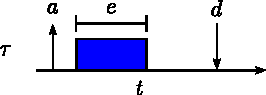
\includegraphics[width=0.50\linewidth]{fig/singleJob.pdf}
    \caption{Real-Time Job Parameters} A single job of task $\tau$ with release time $a$, execution time $e$, and deadline $d$.
    The x-axis is time where an upward arrow indicate the release of a job and a downward arrow represents the deadline of the job.
    The box represents execution time allocated to task $\tau$.
    \label{fig:rt-job}
\end{figure}

\subsubsection{Task}

A task, $\tau_i$, is an infinite series of jobs characterized by the tuple $\tau_i = (a,p,c,d)$ where $a$ is the offset of the task, $p$ is either the period or minimum interarrival, $c$ is the WCET, and $d$ is the relative deadline.
The offset, $a$, is the time after $t=0$ at which the first job of the task is released.
Tasks may be either aperiodic (also known as sporadic) or periodic.
Sporadic tasks release jobs at irregular intervals.
If $\tau$ is a sporadic task, $p$ represents the minimum interarrival time between successive jobs.
Periodic tasks release jobs at regular intervals.
If $\tau$ is a periodic task, $p$ represents the fixed interarrival time between successive jobs.
The WCET, $c$, is the upper bound on execution time for all jobs the task may release.
The relative deadline, $d$, is the relative deadline for all jobs of the task such that a job released at time $t$ is has a deadline at time $t+d$.
Figure \ref{fig:rt-task} illustrates a two tasks, one sporadic and one periodic, and their typical parameters.

\begin{figure}[!htbp]
    \centering
    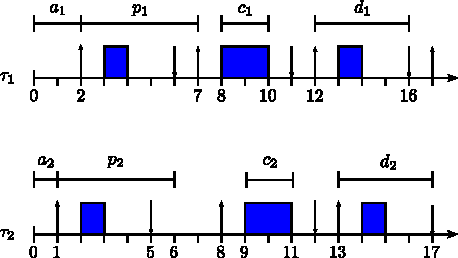
\includegraphics[width=0.75\linewidth]{fig/taskParameters.pdf}
    \caption{Real-Time Task Parameters: Periodic and Sporadic}
    Task $\tau_1 = (a_1=2, p_1 = 5, c_1=2, d_1=4)$ is a periodic task.\\
    Task $\tau_2 = (a_2=1,p_2=5,c_2=2,d_2=4)$ is an aperiodic task.\\
    Note that $\tau_1$, being periodic, has fixed releases $p_1$ units of time apart whereas $\tau_2$, being aperiodic, has releases \textit{at least} $p_2$ units apart.
    \label{fig:rt-task}
\end{figure}

\subsubsection{Task Set}

When more than one task is needed to describe all computational loads, tasks are represented by a task set, $\Tau = \{\tau_1, \tau_2, \dots, \tau_n\}$, a collection of individual tasks.
From this task set, an additional parameter, the Hyperperiod $H$, can be derived.
The hyperperiod $H$ represents the least common multiple (LCM) of all periods (or minimum interarrival times) in  the task set.
Formally, $H = \text{LCM}(p_1, p_2, \dots, p_n)$.
This hyperperiod represents when the pattern of computation repeats.

\subsection{Characterizing Demand}

With some fundamental tools for modeling computation covered, we now describe methods of representing the total computation a task (or set of tasks) may require. 

\subsubsection{Utilization}

One such method is utilization, the ratio of WCET to period.
For an individual task, $\tau_i$, utilization is given by:
\begin{equation}
    u_i = \frac{c_i}{p_i}.
\end{equation}
The utilization for a task set is then,
\begin{equation}
    U = \sum_{i \in \Tau} \frac{c_i}{p_i}.
\end{equation}

Note that while utilization describes the ratio of time consumed to time available, it does not describe the change in computational load over time.

\subsubsection{Demand and the Demand Bound Function}

To provide a more precise representation of computation over time, \textit{demand} is used.
The \textit{demand} over some time interval $[t_1,t_2]$ is the sum of all WCETs of jobs with release time and deadline in the interval.
Figure \ref{fig:demandExample} illustrates how tasks contribute to demand.
Demand, however, only reflects a particular interval of time and not any possible interval.
To address demand over any interval, the Demand Bound Function (DBF) was introduced by Baruah et al. \cite{baruah_preemptively_1990}.
The DBF is a function which characterizes demand by providing the maximum cumulative execution time a set of tasks may require from a processor over any interval of size $\delta$. 
The formal definition presented in Baruah et al. \cite{baruah_preemptively_1990} is used here.
\begin{definition}[Demand bound Function]\label{def:dbf}
    The \textit{demand bound function}, $DBF(\tau,\delta)$, gives the cumulative WCET of all jobs of $\tau$ with both release times and deadlines within any time interval of length $\delta$.
\end{definition}
Note that since the DBF describes demand over any interval, the DBF is typically more complex to calculate than utilization.

\begin{figure}[!htbp]
    \centering
    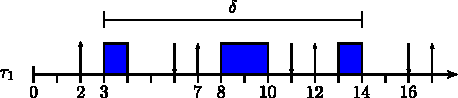
\includegraphics[width=0.75\linewidth]{fig/demandExample.pdf}
    \caption{Real-Time Demand Example}
    Task $\tau_1 = (a_1=2, p_1 = 5, c_1=2, d_1=4)$ is a periodic task.\\
    The \textit{demand} over interval $\delta = [3,14]$ is $2$.
    Since first job's release at time $t=2$ is not in the interval, the WCET of the first job is not counted towards demand.
    The second job's release time and deadline are in the interval so the WCET of the second job counts towards demand.
    The third job deadline at time $t=16$ is not in the interval and thus the WCET of the third job is not counted towards the demand.
    \label{fig:rt-demand}
\end{figure}

\subsection{Feasibility and Schedulability}

With utilization and the DBF as tools for modeling computation, our aim is to determine whether computation can be performed without missing deadlines.
To do so requires generating a schedule that ensures every job of every task is allocated the appropriate processor time to complete its execution before its deadline.
The first step in this process is feasibility analysis.

\subsubsection{Schedules}

To place feasibility and schedulability in context, we first examine schedules.
A \textit{schedule} is an assignment of tasks to a processor (or set of processors) which represents when (and thus, for how long) each job and task is executed.
Formally, a schedule for a single processor is a function which can be given as:
\begin{equation}
    \sigma(t) = i \; | \; t \in \mathbb{R}^+, \; i \in \mathbb{Z}
\end{equation}
where $t$ represents time and $i$ represents the index of the task being executed where index zero is no task (the processor is idle).
Figure \ref{fig:rt-schedule} gives a simple schedule for two tasks.

\begin{figure}[!htbp]
    \centering
    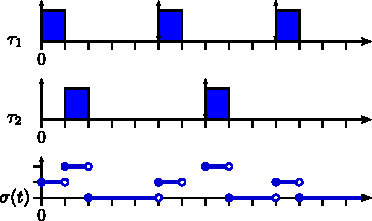
\includegraphics[width=0.5\linewidth]{fig/scheduleExample.pdf}
    \caption{Real-Time Demand Example}
    Task $\tau_1 = (a_1 = 0, p_1 = 5, c_1 = 1, d_1 = 5)$ and is periodic.\\
    Task $\tau_2 = (a_2 = 0, p_2 = 7, c_2 = 1, d_2 = 7)$ and is also periodic.\\
    Note the value of $\sigma(t)$ indicates which task is to be executing\\
    where $\sigma(t) = 0$ indicates no task is scheduled to run.
    \label{fig:rt-schedule}
\end{figure}

Given a set of tasks and processors to execute the tasks on, we now turn our attention to whether any schedule can be made, a process known feasibility analysis, and whether a particular scheduling algorithm algorithm could make a feasible schedule, a process known as schedulability analysis.

A function describing which jobs or tasks are executed.
A map of workloads onto available time.

\subsubsection{Utilization}

\subsubsection{Demand Bound Function}


\subsubsection{Scheduling Algorithms}

An algorithm which takes tasks as inputs and generates a schedule.



\clearpage

%Compile Chapter N
\section{Hardware-Software Codesign of a Short Circuit Detection System}   \label{chap:scd}

In this chapter, a short circuit detection system is proposed in which a real-time task period (or sampling frequency) is directly linked to the current flowing through a monitored power pathway.
This relationship is then used to relate board space on a printed circuit board to the utilization required by the real-time task.

\subsection{Introduction}   \label{subsec:hardwareSoftwarreCodesign}

\paragraph{Motivation and Applications}
From cell phones to solar panels, devices of all sizes require power semiconductors to control, direct, and manage the flow of electricity.
Batteries, CPUs, and photovoltaic inverters all leverage this flow of electricity, known as current, to perform tasks from actuation to computation.
In excess, however, current leads to thermal cycling and can be degrading or destructive to power circuitry.
One cause of excessive current is short circuiting.
A short circuit occurs when current travels through an alternate, unintended path in a circuit often with little or no resistance.
This alternate path of travel with no resistance leads to high current, increased heat, and often circuit damage.
This potential for damage creates a need for short circuit protection.

The need for short protection can be seen in a variety of applications relying on power semiconductors including power converters and inverters \cite{horiguchi_high-speed_2015}.
In an industrial setting, this can include photovoltaic systems and hybrid fuel cells \cite{zhang_model-based_2011}.
In a consumer setting, this can include electric vehicles, laptops, and cell phones like the recent Samsung Galaxy Note 7 which was recalled due to fires caused by short circuits in the device battery \cite{hollister_heres_2016}.

To mitigate the risk of short circuits, devices using power-semiconductors can be constructed with short circuit protection in the form of a fuse, thermal breaker, or other hardware designated to prevent the high current responsible for circuit damage.
This short circuit protection, however, is often fixed circuitry dedicated solely to short detection.
In such systems, little flexibility is afforded to circuits which operate at varying voltages and currents over their lifetime as designers must protect against short circuits at the highest currents and voltages, even if they are not the most frequently used.
Moreover, the rise in semiconductor power density continues to reduce the required latency for detecting and halting shorts \cite{horiguchi_short_2014}.

\paragraph{Problem Statement}
In light of the motivation above, the problem of designing flexible short circuit protection systems can be viewed through the lens of real-time software.
Given the inherent possibility of catastrophic failure in short circuit protection systems and the time-sensitive nature of current rise during short circuits, we seek to frame the problem as one of hardware-software co-design via hard real-time systems.
Specifically, we aim to address the problem of short circuit protection in direct current (DC) resistor-inductor (RL) circuits - circuits containing resistors and inductors where current flows in only one direction.

To address the need for flexible, short circuit protection, our problem statement is:

\noindent Given a Direct-Current Resistor-Inductor circuit, devise a hardware-software co-design approach which relates hard-real time requirements to hardware size.
More specifically, our objective is to construct a hardware-software relationship which allows designers to:
\begin{enumerate}
    \item minimize hardware size while meeting maximum real-time utilization requirements, and
    \item minimize real-time utilization while meeting maximum hardware size requirements.
\end{enumerate}

\paragraph{Proposed Solution}
To address the need for flexible, real-time short circuit protection, we propose a short-protection method via a real-time task as follows:

A DC RL circuit containing an air-core inductor placed in series between the system's resistive load and ground is connected (and controlled) by a microcontroller.
The microcontroller executes a real-time task responsible for sampling voltage across the inductor (or a small resistor) to measure current via an Analog-to-Digital Converter (ADC) pin.
Short protection is accomplished by identifying the maximum expected current and the maximum rate of current change as limited by the circuit's inductor.
Using the inductor spatial parameters in conjunction with ADC sampling times, a minimum sampling period is derived for the real-time task.
From this minimum period, a relationship between minimum real-time utilization under Earliest Deadline First (EDF) scheduling and inductor volume is provided.
Real-time or physical system constraints may be applied to this relationship to facilitate the hardware-software co-design of a real-time short circuit protection system.

This approach is intended to allow existing systems with microprocessors to migrate short circuit protection from dedicated-circuitry-only to a software-based implementation and future systems to be designed with the proposed hardware-software tradeoff in mind.

\paragraph{Contributions}
%Contributions: Long-form writing
The software-based protection methods depicted herein provide an alternative short circuit protection technique to circuit designers.
By relating utilization to the volume of (and board space consumed by) an inductor, system designers may trade short-protection circuitry for real-time task utilization on the microcontroller, leveraging either end of the relationship to meet fault-tolerance and space requirements.
For example, applications with little available board space may opt for smaller inductors (minimizing board space) and greater utilization.
Example applications include smaller IGBT modules as found in electric vehicles or applications where minimizing weight is import\cite{ji_situ_2013}.
In contrast, larger applications with more available board space or a greater real-time task set may opt for a larger inductor and thus a smaller utilization for the short-protection task.
Example applications include high power IGBT modules in photovoltaic and wind turbine inverters \cite{zhang_model-based_2011}\cite{busca_overview_2011}.
Perhaps most importantly, the established relationship between board space and processor utilization acts as a conduit through which advancements in electrical engineering may improve real-time system efficiency and vice versa.
To summarize, our contributions include\footnote{This work was published in the 2017 IEEE 23rd International Conference on Embedded and Real-Time Computing Systems and Applications (RTCSA) under the same title \cite{willcock_trading_2017} and is an extension upon the related senior thesis by Willcock \cite{willcock_short_2016}.}:%Contributions: Bullet-point summary
\begin{description}
\item [1.] a software-based short protection method for Direct Current Resistor-Inductor circuits,
\item [2.] a relationship between air-core inductor spatial parameters and real-time processor utilization under preemptive uniprocessor EDF scheduling for short circuit protection,
\item [3.] a process for identifying optimal inductor orientation given a fixed volume, and
\item [4.] a process for minimizing utilization given a fixed volume for an air-core inductor and vice versa.
%\item [5.] A process for minimizing the required volume for an air-core inductor given a fixed utilization.
\end{description}


%Outline of paper
\paragraph{Outline}
Related work in both the electrical and real-time domain was previously covered in Chapter \ref{chap:relatedWork}.
Section \ref{subsec:electronics background} provides an electronics background and nomenclature overview.
Section \ref{subsec:electronic system model} provides the first paper contribution, a model for identifying circuit properties.
Section \ref{subsec:method of protection} depicts short protection methods given the constraints provided in the circuit model.
Section \ref{subsec:real-time system model} formalizes the relation between real-time scheduling and short circuit protection.
Section \ref{subsec:model optimization} provides the model optimization for both fixed board constraints and fixed real-time utilization as contributions from this paper.
Section \ref{subsec:experiments} details experiments conducted to validate the proposed relationship and theoretical utilization.
Section \ref{subsec:results} discusses the results of experimentation.
Section \ref{subsec:conclusion} identifies conclusions and future work.

%Intersection of EE and RTS
%The problem of protecting electronics from short circuits has traditionally been a concern of electrical engineering and has been addressed through several techniques including current mirrors and clamp circuits \cite{litRev}.
% With the application of real-time software to short protection, we shift the problem to the intersection of electrical engineering, cyber-physical, and real-time systems.
% Thus, solutions are subject to the physical, electronic, and real-time limitations of the system.

%The proposed software-based short circuit protection approach aims to reduce dedicated circuitry on platforms already using a microprocessor and provide an alternative method to short protection.
% The motivation behind this hardware-software co-design approach is the flexibility and ubiquity of microprocessors.
% The potential for movement of protection systems from dedicated circuitry to software implementations [OLD].

\clearpage \subsection{Electronics Background}\label{subsec:electronics background}
The following section covers background required for constructing the proposed circuit model.
It includes an overview of nomenclature, DC RL circuits, inductors, and short circuits.
These electronics fundamentals can be found in a typical collegiate physics textbook \cite{young_sears_2012}.

\paragraph{Nomenclature}
%Define all terms (voltage, current, etc.) and the symbols that represent them.
For the purposes of describing our approach, we rely on the following nomenclature:

\begin{center}
\bgroup
% \def\arraystretch{1.0}%
\begin{tabular}{| l | c | c | c | l |}
    \hline
    Term & Symbol & Unit & Description\\  \hline \hline \cline{1-4}
    Current & I & Ampere (A) & The rate of electric charge flow \\ \cline{1-4}
    Inductance & L & Henry (H) & The ability to induce electromotive force\\ \cline{1-4}
    Voltage & V & Volt (V) & Electric potential difference \\ \cline{1-4}
    \hline  
\end{tabular}
\egroup
\end{center}

\paragraph{First-Order DC RL Circuits}
%Define a DC circuit, Include Figure.
Direct current (DC) circuits are circuits in which the direction of current flow does not change \cite{young_sears_2012}.
A DC circuit in which current passes through a resistor and an inductor is deemed a DC RL circuit where "R" represents the resistor and "L" the inductor.
The model presented in Section \ref{subsec:electronic system model} relies on a first-order DC RL circuit with the resistor and inductor in series.
An example first-order DC RL circuit is provided in Figure \ref{fig:ModelDCRL} with two resistors and an inductor in series.
\begin{figure}
    \centering
    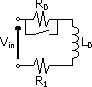
\includegraphics[width=0.25\linewidth]{fig/Model_DC_RL_Circuit_General.pdf}
    \caption{Model DC RL Circuit} A DC RL circuit with load $R_0$, inductor $L_0$, resistor $R_1$, and switch for inducing shorts.
    \label{fig:ModelDCRL}
\end{figure}
%\begin{figure}[!htbp]
%	\centering
%    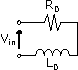
\includegraphics[scale=2.0]{fig/DC_RL_Circuit_General.pdf}
%    \caption{An Example DC RL Circuit}
%    \label{fig:DCRL}
%\end{figure}
\paragraph{Inductors}
An inductor is a passive electronic component typically illustrated as a coil or four- which resists change in current flow through itself.
This property is useful as current through an inductor cannot change instantaneously.
Equations describing these properties are provided in Section \ref{subsec:method of protection}.
\subsubsection{Spatial Parameters}
%Figure of inductor with associated variables, Derivations will be explained later.
The model proposed in Section \ref{subsec:electronic system model} will rely on a single, air-core inductor.
The spatial properties of an inductor may be modeled as seen in Figure \ref{fig:InductorParams}.
\begin{figure}
    \centering
    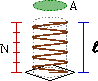
\includegraphics[width=0.25\linewidth]{fig/Inductor_Parameters.pdf}
    \caption[Air Core Inductor Spatial Parameters]{Spatial parameters of an air core inductor}
    \label{fig:InductorParams}
\end{figure}
The figure describes a solenoid-style inductor where $N$ represents the number of complete turns, $A$ is the area of a coil, $\ell$ represents the length of the inductor.
The relationship between these parameters and inductance can be constructed from fundamental electricity and magnetism equations found in Young et al. \cite{young_sears_2012}.
This relationship is modeled as:
\begin{equation}\label{eq:InductorSpatial}
L = \frac{\mu_0 N^{2}A}{\ell}
\end{equation}
where $\mu_0$ is the permeability of free space.
For our purposes, we assume the spatial parameters are fixed -- i.e., $\ell$, $A$, and $N$ are static\footnote{In Section \ref{subsec:model optimization}, we consider variable sized inductors as part of our hardware-software co-design optimization.}.
Equation (\ref{eq:InductorSpatial}) will be referenced in Section \ref{subsec:method of protection} to relate current-flow to inductor size and in Section \ref{subsec:model optimization} to optimize hardware-software co-design solutions.
\subsubsection{Assumption of Constant Turn Density} \label{ssec:Assumption of Constant}
Equation (\ref{eq:InductorSpatial}) contains the term $\frac{N}{\ell}$, referred to as \textit{turn density}.
\textit{Turn density} must remain constant with an increase in length for inductance to increase.
Thus if an inductor is to be extended from length $\ell$ to $2\cdot \ell$, the number of turns $N$ should be doubled accordingly (to $2\cdot N$) to maintain constant \textit{turn density}.
Doubling both $N$ and $\ell$ results in doubled inductance $L$.
Whenever a change in inductor length $\ell$ is suggested, we assume the number of turns is doubled as well to maintain constant \textit{turn density}.
We rely on this assumption throughout Section \ref{subsec:model optimization}.
\subsubsection{Inductor Core Composition}
The core of a solenoid-style inductor can be defined as the area within the coiled wire.
In practice, many inductors are manufactured with ferromagnetic cores which increase the inductance for the same volume.
In our model, we assume this core is empty and contains only air.
Equation (\ref{eq:InductorSpatial}) reflects this assumption as it applies only to air-core inductors.
We view this assumption as an upper bound on board space consumed since ferromagnetic core inductors provide a greater inductance by volume \cite{gao_fabrication_2006}.

\paragraph{Definition of Short and Fault Types}
%Define short in the context of this paper
For the purposes of this model, a short is defined as the flow of current through an alternate, unintended path in a circuit with little or no impedance.
In the event of a short, this loss of impedance causes a large change in current which can be slowed and detected through careful reliance on an inductor's ability to resist instantaneous changes in current.
However, short circuits lead to joule heating, the process whereby current through a conductor releases heat modeled as:
\begin{equation}\label{eq:JouleHeating}
\text{Heat} \propto R I^{2} t
\end{equation}
Here, $R$ is resistance, $I$ is current, and $t$ is time \cite{young_sears_2012}.
The thermal buildup from joule heating is responsible for the permanent damage that can result from a short and therefore serves as motivation for short circuit protection.
Protection from damage, however, requires catching two short circuit fault types: the Fault under Load (FUL) and the Hard-Switching Fault (HSF).

\subsubsection{Fault Under Load vs Hard-Switching Fault}
In the context of short circuit protection, a Fault Under Load is a short circuit fault where a circuit has an active load at the time of the fault.
In this type of fault, the current and impedance are both non-zero.
Intuitively, this means the circuit is "on" at the instant the short circuit occurs.
The short forces current to rise, often above desired operating ranges.
This fault type, commonly analyzed in IGBTs, has been studied in Pagano et al. \cite{pagano_short_2005}.

In contrast, a Hard-Switching Fault is a short circuit fault where the circuit does not have an active load at the time of the fault \cite{horiguchi_high-speed_2015}.
In contrast to an FUL, an HSF does not have an initial operating current since there must be a short circuit path before the circuit is "on".

\paragraph{Current as a Function of Time}
In the proposed system, a real-time task must be related to the change in current through an inductor.
The following equation will provide such a relationship used Section \ref{subsec:method of protection}:
\begin{equation}\label{eq:CurrentAtTime}
I(t) = \frac{V}{R}(1-e^{-t \frac{R}{L}})
\end{equation}
where $I(t)$ is current at time $t$, $V$ is a constant voltage to the circuit, $R$ is resistance, and $L$ is inductance.
\clearpage \subsection{Electronic System Model}\label{subsec:electronic system model}
%Define the system model and its components (DC RL Circuit, the OCM)
In the previous section, an electronics background was provided as context for our approach.
In this section, we will define and describe the system model from an electronics perspective.
Relying on the provided background, we propose an electronics model with four primary components:
\begin{description}
\item [1.] a DC RL circuit to which software-based short circuit protection is applicable and board space is consumed by air-core solenoid-style inductor,
\item [2.] an Operating Current Model (OCM) to characterize first-order DC RL circuits,
\item [3.] two short circuit detection methods for first-order DC RL circuits, and
\item [4.] a real-time sporadic task for short protection.
\end{description}

The short circuit detection methods will be discussed in Section \ref{subsec:method of protection} and the real-time model (and its utilization analysis under uniprocessor EDF scheduling) will be discussed in Section \ref{subsec:real-time system model}.

\paragraph{DC RL short circuit Schematic}
Figure \ref{fig:ModelDCRL} is a model DC RL circuit with a switch for simulating a short circuit.
This schematic provides the requirements for the monitored, short-protected circuit: a voltage supply $V_{in}$, circuit load $R_{0}$, inductor $L_{0}$, and the optional, low-value resistor $R_{1}$ used for sensing current.
If $R_{1}$ is not used, the resistance through inductor $L_{0}$ may be used to calculate current.
Note that the short occurs via the switch around $R_{0}$.
%    \begin{figure}
%    	\centering
%        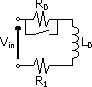
\includegraphics[scale=2.0]{fig/Model_DC_RL_Circuit_General.pdf}
%        \caption{A DC RL circuit with load $R_0$, inductor $L_0$, optional resistor $R_1$ and switch for simulating potential shorts.}
%        \label{fig:ModelDCRL}
%    \end{figure}

As previously mentioned, in a manufactured circuit the spatial parameters and inductor value of $L_0$ in Figure \ref{fig:ModelDCRL} are expected to be fixed.
During the design phase however, inductor parameters may be altered to increase space efficiency.
These properties are afforded by Equation (\ref{eq:InductorSpatial}).

\paragraph{Board Space Consumed}
\begin{figure}
    \centering
    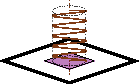
\includegraphics[scale=2.0]{fig/Inductor_Perpendicular_Mount.pdf}
    \caption{Board Space Consumed by an Air-Core Solenoid-Style Inductor} The highlighted square circumscribing area $A$ of the inductor represents the board space consumed by a solenoid-style air-core inductor.
    \label{fig:BoardSpaceConsumed}
\end{figure}
For ease of analysis, we assume the axis of the inductor is mounted perpendicular to the board as shown in Figure \ref{fig:BoardSpaceConsumed}.
Therefore, the board space consumed by the inductor is defined as the square that circumscribes area $A$ of the inductor as seen in Figure \ref{fig:InductorParams}:
\begin{equation}\label{eq:AreaConsumed}
A_{consumed} = \frac{4}{\pi}A
\end{equation}
This definition of board space consumed will be referenced in Section \ref{subsec:model optimization} where the provided model is optimized for minimum board space consumption and volume.
\paragraph{Operating Current Model}
To simplify the analysis of DC RL circuits, we propose an Operating Current Model (OCM) for characterizing the circuit's maximum current, maximum voltage, and critical current.
Hereafter, we model DC RL circuits as:
\begin{equation}\label{eq:OCM}
C = (\Gamma_{I}, I_{crit})
\end{equation}
where $C$ is the circuit described using parameters $\Gamma_{I}$ and $I_{crit}$.
$\Gamma_{I}$ is defined such that:
\begin{equation}\label{eq:OCMTuples}
\Gamma_{I} = (\gamma_{1},\gamma_{2},...,\gamma_{n})
\end{equation}
\begin{equation}\label{eq:OCMIVPairs}
\gamma_{i} = (I_{i},V_{i})\qquad\text{for all  } i=1,...,n
\end{equation}
Here $\Gamma_{I}$ is composed of $n$ operating current sets $\gamma_{i}$ where $i$ is the index of an operating current set.
Each operating current set is a 2-tuple of an operating current, $I_{i}$, and operating voltage, $V_{i}$.
The resistance, $R$, of each operating current set can be solved using Ohm's Law and is not included.

$I_{crit}$ is defined as the critical current of the system as determined by the user.
The critical current represents the current value at which the system physically degrades or, in practice, the current value the user wishes to avoid reaching.

Two final derivable parameters $I_{max}$ and $V_{max}$, are extracted from the OCM as follows:
\begin{equation}\label{eq:Imax}
I_{max} = \max_{i \in \Gamma_{I}} \{\gamma_i\} \quad \text{and} \quad V_{max} = \max_{i \in \Gamma_{I}} \{\gamma_i\}
\end{equation}
Note that if $I_{crit} = I_{max}$, any current flow over $I_{max}$ is assumed to be damaging and may not be prevented through this short protection model.
Thus, we assume $I_{max} < I_{crit}$.
\clearpage \subsection{Methods of Protection}\label{subsec:method of protection}
%Overview of the methods of short protection.
The intersection of electronics modeling and real-time systems begins with strategies for detecting and halting short circuits.
To detect a short in the generalized first-order DC RL circuit, as seen in Figure \ref{fig:ModelDCRL}, we present two methods for detection:
\begin{description}
\item [1.] a simple comparison of current, $I$, against maximum current, $I_{max}$ and
\item [2.] a comparison of change in current, $\Delta I$, against the maximum change in current, $\Delta I_{\max}$, allowed.
\end{description}
Both methods are applicable to any system which samples current of a monitored circuit.
To prevent damage from shorts and fully utilize the following protection methods, power to the monitored circuit(s) must be removed immediately upon detection of a short.
Without removal of power, these methods merely support detection and not protection.
\paragraph{Method 1: Maximum Operating Current}
The first method for detecting short circuits in a DC RL circuit is to identify when current rises above $I_{max}$.
A current value above $I_{max}$ indicates some malfunction caused current to rise above the maximum current in the OCM.
When $I > I_{max}$, power to the monitored circuit should be disabled to protect the hardware.
\paragraph{Method 2: Maximum Change in Current}
%Define the dI/dt method
The second method of detection requires observing the rate of change of current.
From Equation (\ref{eq:CurrentAtTime}) it is known that, given a constant voltage and resistance, the current will converge to $\frac{V}{R}$.
During convergence, the slope of $\Delta I$ approaches zero.
The derivative of Equation (\ref{eq:CurrentAtTime}) provides the value of $\Delta_{\max}I$:
\begin{equation}
\Delta I = \frac{\partial}{\partial t}I(t) = \frac{\partial}{\partial t}(\frac{V}{R}(1-e^{-t \frac{R}{L}})) = \frac{V}{L}e^{-t \frac{R}{L}}
\end{equation}
Assuming constant inductance, resistance, and voltage, the largest values of $\Delta I$ occur at $t = 0$ and $R = 0$ while excluding infinite inductance ($L \neq +\infty$).
This leads to the following conclusions:
\begin{description}
\item [1.] If $R \neq 0$, $\frac{dI(t)}{dt} = \frac{V}{L}$ instantaneously at time $t = 0$ only.
Assuming no short has occurred, the change in current between any two consecutive current samples should be less than $\frac{V}{L}$.
Formally, $\forall \delta > 0, t \geq 0, \frac{|I(t+\delta) - I(t)|}{\delta} < \frac{V}{L}$ 
\item [2.] If the change in current between two consecutive current samples is equivalent to $\frac{V}{L}$, then $R = 0$ and a short is occurring.
\end{description}

We can safely state the maximum $\Delta I$ through an inductor at any time $t$, including $t = 0$, is:
\begin{equation}\label{eq:DeltaMax}
\Delta_{\max}I = \frac{V}{L} \nonumber
\end{equation}
Since all non-superconducting materials will provide some impedance, the $\Delta_{\max}I$ should have a threshold, $\epsilon$, which serves as an implementation-specific offset.
When consecutive current samples are compared, $\Delta_{\max} I = \frac{V}{L} - \epsilon$ should be used as the point of comparison.
If a $\Delta I \approx \Delta I_{\max}$, it is likely that $R \approx 0$ and a short is occurring.
A benefit of using $\Delta_{\max}I$ is the potential for short detection before $I_{max}$ has been reached.
In HSFs, there is no initial current ($I(0) = 0$) which could allow $\Delta I$ to approach $\Delta_{\max}I$ before $I$ exceeds $I_{max}$.
\paragraph{Time-to-Detection}
The previous section discussed methods of detecting short circuits which cover the logical requirements of the real-time short-protection task but did not provide any explicit temporal constraints.
As previously mentioned, short-protection systems are time-sensitive and a valuable short circuit detection occurs before critical current levels are reached.
To do so requires determining the time taken for current to rise from its present value, $I$, to the critical current, $I_{crit}$.
For the remainder of this paper, we deem this the \textit{time-to-detection}.

\subsubsection{Arbitrary Operating Voltage}
%Define minimum time-to-detection
If the OCM for the circuit in question contains a single operating voltage, it must hold that:
\begin{equation}\label{eq:SingleV}
\forall  V  \in \Gamma_{I}, V = V_{max}
\end{equation}
If Equation (\ref{eq:SingleV}) holds, the \textit{time-to-detection}  is:
\begin{equation}\label{eq:TimeToDetect}
\delta(I,V) = \frac{I_{crit}-I}{V}\cdot L
\end{equation}
where $\delta(I,V)$ is \textit{time-to-detection}, $I$ is current, $I_{crit}$ is the critical current, $V$ is voltage, and $L$ is inductance.
The function provides the time required for current to rise from $I$, to the critical current, $I_{crit}$, in a DC RL circuit with voltage $V$ and inductance $L$.
This function demonstrates that lower currents and voltages provide a lower \textit{time-to-detection}.
    
However, to use this function for identifying the smallest time-to-detection in an OCM with multiple voltages would be optimistic.
Suppose, for example, a DC RL circuit allows for two operating voltages, $V_\ell$ and $V_h$ such that $V_\ell < V_h$.
Suppose now that at the instant a short circuit occurs the operating voltage increases from $V_\ell$ to $V_h$.
The value of $\delta(I,V_\ell)$, calculated before the short circuit ocurred, will be an overestimate of the time required for $I$ to exceed $I_{crit}$.
To address this, we define the 

\subsubsection{Maximum Operating Voltage}
Since using Equation (\ref{eq:TimeToDetect}) becomes optimistic when multiple operating voltages are involved, we can remove optimism by replacing $V$ from Equation (\ref{eq:TimeToDetect}) with $V_{max}$:
\begin{equation}\label{eq:TimeToDetectVmax}
\delta(I,V_{max}) = \frac{I_{crit}-I}{V_{max}}\cdot L
\end{equation}
Equation (\ref{eq:TimeToDetectVmax}) ensures a short combined with an instantaneous voltage change to $V_{max}$ is still detected before reaching $I_{crit}$.

\subsubsection{Minimum Time-to-Detection}
%Define minimum time-to-detection
To provide the worst-case time-to-detection, we use the maximum current, $I_{max}$ and voltage, $V_{max}$, from the OCM.
This \textit{minimum time-to-detection} is defined as:
\begin{equation}\label{eq:MinTimeToDetect}
\delta_{min} = \delta(I_{max},V_{max}) = \frac{I_{crit}-I_{max}}{V_{max}}\cdot L
\end{equation}
This time frame represents time taken for current to rise from the maximum operating current, $I_{max}$, to the critical current, $I_{crit}$, with the highest voltage, $V_{max}$.
This \textit{minimum time-to-detection} will be used as a temporal constraint for the proposed real-time task.
\clearpage \subsection{Real-time System Model}\label{subsec:real-time system model}
%Overview of real-time systems.
Thus far, the spatial properties of an inductor have been related to its inductance.
Thereafter, inductance is found to determine the maximum possible current rise at any given time, $\frac{V}{L}$ Amperes per second.
This leads to the shortest time span over which a short would need to be detected, the \textit{minimum time-to-detection} $\delta_{min}$.
Using $\delta_{min}$, we provide a real-time system short circuit protection task and its timing requirements.
Before doing so, we present a real-time background on the sporadic task model and uniprocessor EDF scheduling.

\paragraph{Sporadic Task Model}
In real-time systems, \textit{sporadic tasks} are defined by a \textit{worst-case execution time} (WCET) $e_{i}$, relative deadline $d_{i}$, and minimum period $p_{i}$.
The relative deadline is the time between each job arrival and its deadline.
The minimum period is the smallest time between successive job arrivals.
We use a sporadic task to model the short circuit protection task \cite{mok_fundamental_1983}.
The proposed sporadic task will have an \textit{implicit deadline} where a new job of the short circuit task $\mathrm{T}_{scd}$ may arrive at the absolute deadline of the previous job.

For our short circuit task $\mathrm{T}_{scd}$, the execution time depends on the short circuit protection algorithm used, processor speed, and ADC conversion time.
Thus, the execution time is not assessed here but modeled as $e_{scd}$.

The minimum period, however, is derived from Equation (\ref{eq:TimeToDetectVmax}) which provides a scaling \textit{time-to-detection}.
The minimum period of the sporadic task must be half the value of the \textit{minimum time-to-detection}.
This is required to ensure one full job of $\mathrm{T}_{scd}$ is completed strictly after the short circuit begins.
This requirement is demonstrated in Figures \ref{fig:shortedschedule} and \ref{fig:stoppedschedule} where $\mathrm{T}_{scd}$ executes with a period equal to $\delta_{min}$ and $\frac{\delta_{min}}{2}$.
Recall that $\delta_{min}$ time units after a short, the current level has reached a $I_{crit}$.
Each sporadic job is triggered $\delta(I,V_{max})/2$ seconds after the release of the preceding job, allowing release times to scale with current.
The temporal requirements may be converted into a real-time sporadic task $\mathrm{T}_{scd} = (e_{scd}, p_{scd})$ with the following parameters:
\begin{equation}\label{eq:ExecutionTime}
e_{scd} = \textit{worst case execution time }\text{of short circuit algorithm}
\end{equation}
\begin{equation}\label{eq:Period}
p_{scd} = \frac{\delta(I_{max},V_{max})}{2}
\end{equation}
\begin{figure}
    \centering
    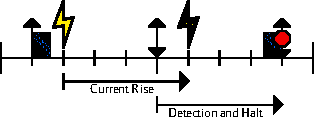
\includegraphics[width=0.60\linewidth]{fig/shortedschedule.pdf}
    \caption{Short Protection Schedule: Failure} $\mathrm{T}_{scd}$ executing with $p_{scd} = \delta(I_{max},V_{max}) = 4$.\\The short begins at $t = 2$ and $I_{crit}$ is reached at $t = 6$ before $\mathrm{T}_{scd}$ can halt the short.
    \label{fig:shortedschedule}
\end{figure}
\begin{figure}
    \centering
    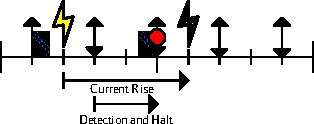
\includegraphics[width=0.60\linewidth]{fig/stoppedschedule.pdf}
    \caption{Short Protection Schedule: Successful} $\mathrm{T}_{scd}$ executing with $p_{scd} = \frac{\delta(I_{max},V_{max})}{2} = 2$.\\The short begins at $t = 2$ and is halted by $\mathrm{T}_{scd}$ at $t = 5$ before $I_{crit}$ is reached.
    \label{fig:stoppedschedule}
\end{figure}
%Game Fucking Over
\paragraph{Preemptive Uniprocessor EDF Scheduling}
%Cite optimality of uniprocessor preemptive EDF scheduling
%Cite utilization calculation for uniprocessor preemptive EDF scheduling.
With $\mathrm{T}_{scd}$ defined, we derive its utilization under preemptive uniprocessor EDF scheduling.
According to \cite{liu_scheduling_1973}, a set of implicit-deadline sporadic tasks is schedulable with EDF if and only if:
\begin{equation}\label{eq:EDFUtilization}
\sum_{i=1}^{n} \frac{e_{i}}{p_{i}} \leq 1
\end{equation}
where $i$ is the index of a task in the set, $e_{i}$ is the execution time, and $p_{i}$ is the period.
Since we use a single, sporadic task with implicit deadlines, the utilization for $\mathrm{T}_{scd}$ is:
\begin{equation}\label{eq:SCDUtilization}
U(\mathrm{T}_{scd}) = \frac{2 \cdot e_{scd}}{\delta(I,V_{max})}
\end{equation}
Using the \textit{minimum time-to-detection}, Equation (\ref{eq:SCDUtilization}) becomes:
\begin{equation}\label{eq:SCDMinUtilization}
U(\mathrm{T}_{scd}) = \frac{2 \cdot e_{scd}}{\delta(I_{max},V_{max})}
\end{equation}
Substituting in Equations (\ref{eq:TimeToDetect}) and (\ref{eq:InductorSpatial}) gives:
\begin{equation}\label{eq:SCDSpatialUtilization}
U(\mathrm{T}_{scd}) = (\frac{2 \cdot e_{scd}}{(I_{crit}-I_{max})} \cdot V_{max} \cdot \frac{\ell}{\mu_0 N^{2}A})
\end{equation}
Equation \ref{eq:SCDSpatialUtilization} relates the inductor spatial parameters to $\mathrm{T}_{scd}$ utilization.

%\paragraph{Detection as a Hard Real-Time Task}
%As previously mentioned, the correctness of a real-time computation has a temporal component, in this case the relative deadline.
% A real-time task in which results produced after a deadline have some utility is a \textit{soft} real-time task.
% Video rendering could be considered a soft real-time task.
% One in which a result produced after a deadline has no utility but results in no damage is considered \textit{firm}.
% In the case of the proposed real-time task, results produced after a deadline may cause have disastrous consequences including damage to the controlled system \cite{rts}.
%\clearpage \subsection{Real-time Utilization Requirement for Short Detection}

\clearpage \subsection{Model Optimization}\label{subsec:model optimization}
Having related the board space consumed by an inductor and the real-time utilization under EDF schedulability, we propose an optimal solution for fixed values on either end of the relationship.
Given a fixed utilization we propose a minimized board space consumption.
Given a fixed allowable board space, we propose a minimized real-time utilization.
Before optimization analysis of the model, we clarify the optimal inductor orientation for a given prism.

\paragraph{Optimal Inductor Orientation}
In practice, hardware-software co-design is constrained by real-world factors such as size, weight, power, and cost.
In this paper, we focus on space as a constraint on our proposed model.
Given a fixed volume of space to implement the proposed short-protection system, we must consider the optimal orientation of our solenoid-style air-core inductor inside the fixed volume which maximizes inductance.
To find the inductor orientation providing the highest inductance for a given space, we consider two constraints:
\begin{description}
\item [1.] The area $A$ from Equation (\ref{eq:InductorSpatial}) requires a square area with regard to board space.
\item [2.] The board space must be defined in three dimensions: a length $\ell$, width $w$, and height $h$.
\end{description}
Allowable board space is therefore defined as a set:
\begin{equation}\label{eq:Prism}
P = \{\ell,w,h\}
\end{equation}
This set provides the prism dimensions in which the inductor resides.
Independent of the prism's orientation, $A_{consumed}$ must be the smallest square to circumscribe the area $A$ of the inductor.
The largest square face on which the inductor's area, $A$, can be placed is limited by the median dimension in P.
Thus, the square of the median is used to fit the largest possible square area:
\begin{equation}\label{eq:PrismAreaConsumed}
A_{consumed} = median(P)^2
\end{equation}
The only remaining dimension is deemed the length of the inductor:
\begin{equation}\label{eq:PrismLength}
\ell = min(P)
\end{equation}

A visualization of possible orientations can be found in Appendix \ref{appendix:orientation-visualization} along with an explicit example.
As previously mentioned and validated in Section \ref{ssec:Assumption of Constant}, the \textit{Assumption of Constant Turn Density} applies to $\ell$ and is required for the remaining model optimization.


\paragraph{Fixed Board Constraints}

Having defined equations for consumed area in terms of the volume allotted for the inductor, we address the first optimization problem where the board space is constrained.
This approach is useful in situations where the embedded application, or the region of space allotted for short circuit protection hardware, is restricted in size.
Suppose allotted board space is restricted to the prism:
\begin{equation}\label{eq:Prism2}
P = \{\ell, w, h\} \nonumber
\end{equation}
where each element of the set is defined in meters.
Combining Equations (\ref{eq:AreaConsumed}) and (\ref{eq:PrismAreaConsumed}) for the area of the inductor $A$ gives:
\begin{equation}\label{eq:InductorAreaPrism}
A = \frac{\pi}{4} A_{consumed} = \frac{\pi}{4} \cdot median(P)^2 \nonumber
\end{equation}
By substitution of Equation \ref{eq:InductorAreaPrism} into Equation (\ref{eq:SCDSpatialUtilization}), the utilization requirement becomes:
\begin{equation}\label{eq:MinUtilizationPrism}
U(\mathrm{T}_{scd}) = \frac{2 \cdot e_{scd} \cdot V_{max} \cdot min(P)}{(I_{crit}-I_{max}) \cdot \mu_0 \cdot N^{2} \cdot \frac{\pi}{4} \cdot median(P)^2}
\end{equation}
The equation above gives us a minimum utilization requirement for meeting short circuit protection requirements given the constrained board space and OCM - which provides $I_{crit}$ and $I_{max}$.

\paragraph{Fixed Utilization}
Having addressed the fixed-volume constraint, we not address the second approach by fixing the maximum utilization allowed short circuit protection process.
This approach is useful in situations where the microprocessor executing $\mathrm{T}_{scd}$ is responsible for other tasks which inherently limit $U(\mathrm{T_{scd}})$.
Suppose the allotted utilization is $u$.
Relying on Equation (\ref{eq:SCDMinUtilization}) we find the minimum time-to-detection $\delta(I_{max},V_{max})$ is solved as:
\begin{equation}\label{eq:MinTimeToDetectSpatial}
\delta_{min} = \delta(I_{max},V_{max}) = \frac{2 \cdot e_{scd}}{u} \nonumber
\end{equation}
Applying Equation (\ref{eq:MinTimeToDetect}) and isolating $L$ we find:
\begin{equation}\label{eq:InductorFixedUtilization}
L = \frac{2 \cdot e_{scd} \cdot V_{max}}{u \cdot (I_{crit}-I_{max})} \nonumber
\end{equation}
Substituting Equation (\ref{eq:InductorSpatial}) in for $L$ 
%gives:
%\begin{equation}\label{eq:MinPrismUtilizationUnsolved}
%\frac{\mu_0 N^{2}A}{\ell} = \frac{2 \cdot e_{scd} \cdot V_{max}}{u \cdot (I_{crit}-I_{max})} \nonumber
%\end{equation}
and isolating inductor spatial parameters results in:
\begin{equation}\label{eq:MinPrismUtilizationUnsolved2}
\frac{A}{\ell} = \frac{2 \cdot e_{scd} \cdot V_{max}}{u \cdot (I_{crit}-I_{max}) \cdot \mu_0 \cdot N^{2}} \nonumber
\end{equation}
Finally, substituting the prism area consumed (Equation \ref{eq:PrismAreaConsumed}) and prism length (Equation \ref{eq:PrismLength}) into Equation \ref{eq:MinPrismUtilizationUnsolved2} above gives:
\begin{equation}\label{eq:MinPrismUtilization}
\frac{median(P)^{2}}{min(P)} = \frac{4}{\pi} \cdot \frac{ 2 \cdot e_{scd} \cdot V_{max}}{u \cdot (I_{crit}-I_{max}) \cdot \mu_0 \cdot N^{2}}
\end{equation}
This result indicates the air core inductor used in the DC RL circuit must have a minimum allotted board space defined by P which satisfies the above equation.

The model optimizations above highlight how fixed board space can be used to prescribe a minimum utilization and vice versa.
We now seek to validate our short circuit protection model in the next section where we discuss our experiments and subsequently our results.

\clearpage \subsection{Experiments}\label{subsec:experiments}
To implement and validate the application of the software-based approach, we conducted four separate experiments.
The following section presents the experiment setup and outlines the conducted experiments.
Additionally, the projected utilization for the experiments is presented.

\paragraph{Experiment Outline}
The experiments conducted measured both FUL and HSF short circuits focusing primarily on FUL short circuits as they have a smaller time-to-detection.
Table \ref{tab:ExperimentDescriptions} highlights the variations between experiments which can be summarized as follows:
Experiment 1 examines the performance of our approach under FUL short circuits in terms of detection latency and maximum current reached at the time of detection.
Experiment 2 examines the performance under HSF short circuits also in terms of latency and maximum current reached at the time of detection.
Experiment 3 demonstrates how fixing utilization and varying inductance under FUL short circuits relates to current at the time of detection.
Experiment 4 demonstrates the same relationship but with varying utilization and fixed inductance.
\begin{table}[!h]
    \centering	
    \bgroup
    \def\arraystretch{1.00}%  1 is the default, change whatever you need
    \begin{tabular}{| c | c | c | c |}
            \hline			
            Experiment & Fault Type & Demonstrates\\ \hline \hline \cline{1-3}
            1 & FUL & Baseline\\ \hline
            2 & HSF & Lower initial $I$\\ \hline
            3 & FUL & Scaling $L$\\ \hline
            4 & FUL & Scaling $U$\\ \hline  
    \end{tabular}
    \egroup
    \caption{Experiment Descriptions}
    \label{tab:ExperimentDescriptions}
\end{table}

\paragraph{Setup}
Aside from the variations described above, all experiments were conducted as described here.
short circuit protection for each experiment was performed on Microchip's DM164103-4 demo board with a PIC18F45K20 CPU.
The demo board and programmer were selected for their relatively low cost to encourage reproducibility.
Figure \ref{fig:ExperimentSetup} depicts the experimental circuit schematic.
In the schematic, subscripts \textit{DM} refer to connections made to the Microchip demo board.
The setup also requires attaching oscilloscope probes to ports RA2 in Figure \ref{fig:ExperimentSetup} and RA1 on the demo board.
Figure \ref{fig:Experiment1Setup} depicts the proper connection of all materials in Experiment 1.
All probe connections route off-camera to the oscilloscope.
An extended list of non-trivial materials used in the experiments can be found in Appendix \ref{appendix:scd-materials}.
\begin{figure}
    \centering
    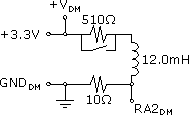
\includegraphics[width=0.45\linewidth]{fig/Experiment_Setup.pdf}
    \caption{Short Circuit Experiment Setup Schematic} Short Circuit Experiment Setup Schematic
    \label{fig:ExperimentSetup}
\end{figure}

\begin{figure}
    \centering
    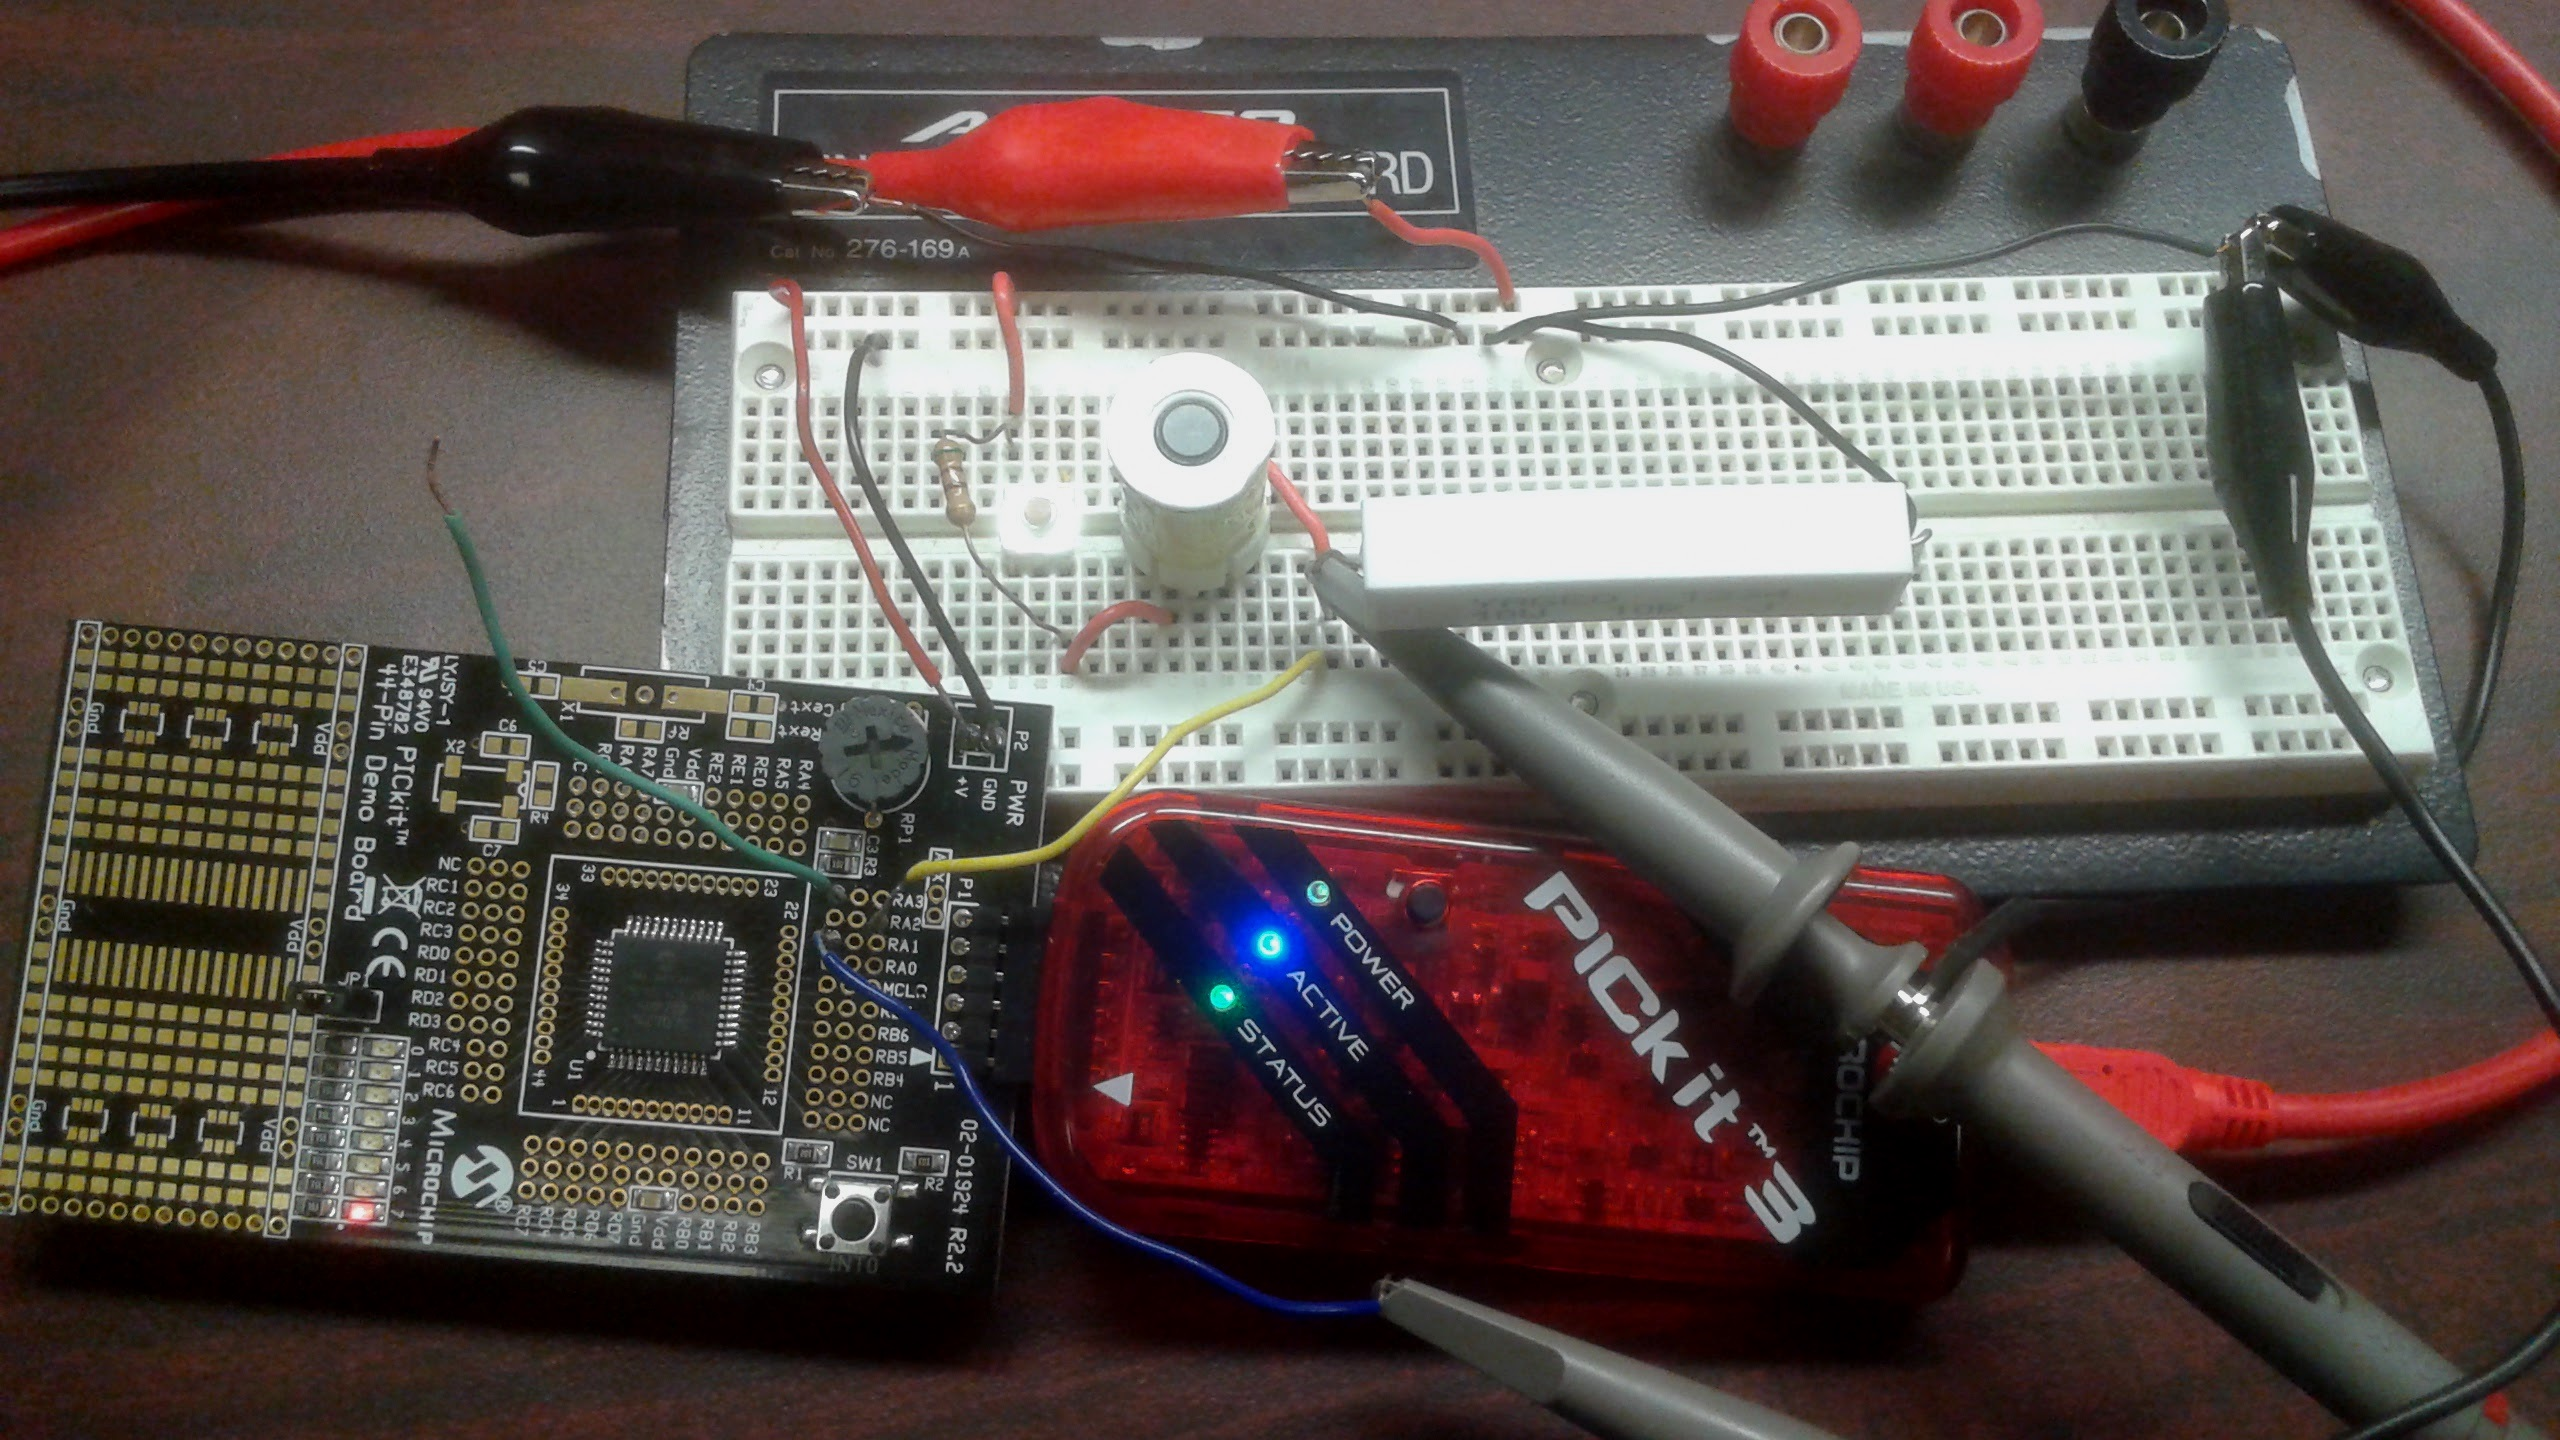
\includegraphics[width=0.75\linewidth]{fig/SCD_5_9mH_EXP_SETUP.jpg}
    \caption{Short Circuit Experiment Setup Image}
    \label{fig:Experiment1Setup}
\end{figure}

The circuit was run in advance of experiments to identify experimental operating currents and voltages and their respective maximums.
This process could be avoided by analyzing the tolerance values for all components used but was explicitly measured here to provide exact values.
The OCM for the setup using solid, 22 American Wire Gauge (AWG) copper wire was:
\begin{equation}\label{eq:OCMSetup}
C = (\Gamma_{I}, 150mA) \quad \Gamma_{I} = (\gamma_{0}) \quad \gamma_{0} = (7.74mA, 3.3V) \nonumber
\end{equation}

Although the resistor $R_{1}$ pictured in \ref{fig:Experiment1Setup} is a 10W power resistor capable of handling higher current, we defer to the power rating of a conventional though-hole power resistor which we assume to be 0.5 Watts.
Since 150 mA through a 0.5 Watt resistor exceeds the power rating at an operating voltage of 3.3 V, 150 mA is considered the critical current $I_{crit}$ for the circuit.

After deriving the OCM from the circuit, Equation (\ref{eq:Imax}) provides the maximum operating current and voltage:
\begin{equation}
I_{max} =  7.74mA \nonumber \quad V_{max} = 3.3V \nonumber
\end{equation}
Note that the critical current is 150mA meaning current above 7.74mA is considered unexpected behavior while current at or above 150mA is damaging.
Having constructed the mathematical model of our system, we may now project the utilization requirement in the following section.

%TODO - Delete?
%Using the OCM, values for $I_{max}$ and $\Delta_{\max}I$ can be converted to the appropriate ADC values.
%Conversion of the ADC resolution to $\frac{\text{Volts}}{\text{ADC Tick}}$ is left to the reader as it is system-dependent.
%The resolution is then used to convert $I_{max}$ and $\Delta I$ to ADC values.
\paragraph{Projected Utilization}
Using the OCM derived from the experiment setup, we apply Equations \ref{eq:SCDUtilization} and \ref{eq:SCDMinUtilization} as the scaling utilization and minimum utilization.
For this projected utilization, our protection method required an execution time of 25 microseconds.
Figure \ref{fig:Simulated Utilization} depicts the projection of fixed minimum utilization and the scaling utilization.
The minimum utilization indicates the expected minimum utilization required to detect a short circuit in the experiment.
The scaling utilization represents the minimum utilization required at \textit{any} given value of $I$ as derived from Equation (\ref{eq:SCDUtilization}).
These projected utilizations indicate the provided short-protection approach could safely detect and halt a short circuit before critical current levels are reached at a uniprocessor utilization of under 0.1.
The scaling utilization curve indicates the lower minimum utilization requirement for systems with lower operating currents.

\begin{figure}
\centering
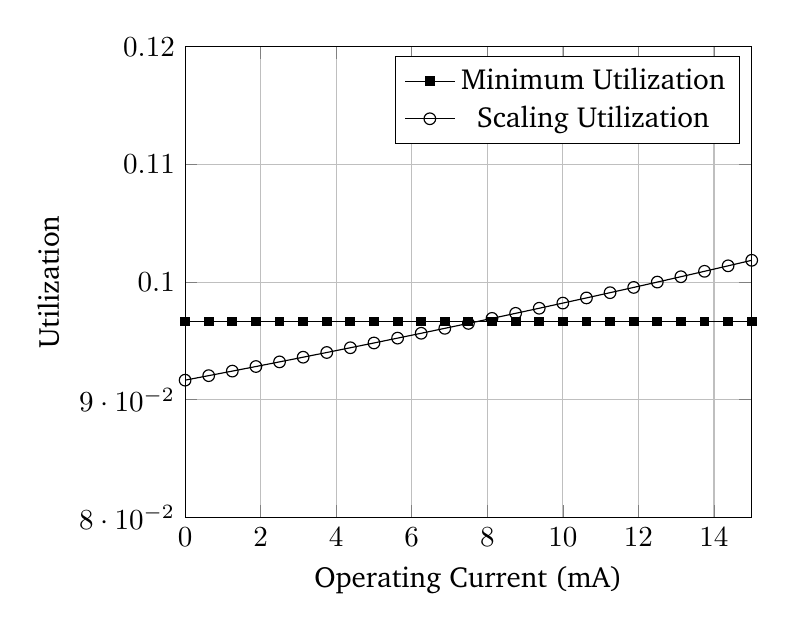
\begin{tikzpicture}[scale=1.05]
    \begin{axis}[ 
    xlabel=Operating Current (mA),
    ylabel=Utilization,
    grid=major,
    xmin=0.00,xmax=15.0,
    ymin=0.08,ymax=0.12
        ] 
    \addplot [mark size=1.5, mark=square*, domain=0:15, samples=25]{(2*0.000025*3.3)/(0.0120*(150 - 7.74))*1000};
    \addplot [mark size=2.0, mark=o, domain=0:15, samples=25]{(2*0.000025*3.3)/(0.0120*(150 - x))*1000};
    \legend{Minimum Utilization,Scaling Utilization}
    \end{axis}
\end{tikzpicture}
    \caption{Simulated Short Circuit Detection Utilization vs. Operating Current}
    \label{fig:Simulated Utilization}
\end{figure}

\clearpage \subsection{Results}\label{subsec:results}
\paragraph{Experiments 1 and 2: FUL and HSF Detection}
To validate the hardware-software co-design approach, two short circuit fault types were induced in separate experiments.
As shown in Table \ref{tab:ExperimentDescriptions}, Experiment 1 induced an FUL short while Experiment 2 inducted an HSF short.
Each experiment was run three times with all data provided in Table \ref{tab:FULHSFComparison}.
In the table, $I_{c}$ is the current at the time of detection and $\Delta t$ is the latency between short circuit and detection.
Three runs per fault type was selected due to time required to manually induce the short and reset each experiment.

\begin{table}
    \centering
    \bgroup
    \def\arraystretch{1.25}%  1 is the default, change whatever you need
    \begin{tabular}{| c | c | c | c | c |}
            \hline			
            Fault & R (Ohm) & $I_{c}$ (mA) & $\Delta t$ (us) & U($\mathrm{T}_{scd}$)\\ \hline \hline \cline{1-5}
%  		FUL & 510 & 31.867 & 132.27 & 0.1316\\  \hline %Original Averages
%  		HSF &   0 & 33.733 & 117.59 & 0.1316\\  \hline %Original Averages
        FUL & 510 & 42.400 & 159.79 & 0.1316\\ \hline
        FUL & 510 & 38.800 & 142.59 & 0.1316\\	\hline
        FUL & 510 & 20.000 &  50.39 & 0.1316\\	\hline
        HSF &   0 & 35.200 & 149.60 & 0.1316\\	\hline
        HSF &   0 & 35.200 &  72.01 & 0.1316\\	\hline
        HSF &   0 & 35.200 & 175.20 & 0.1316\\	\hline
        \end{tabular}
    \egroup
    \caption{FUL and HSF Comparison}
    \label{tab:FULHSFComparison}
\end{table}

Both experiments demonstrate successful detection of FUL and HSF short circuits before current rises above $I_{crit}$.
Both experiments also demonstrate latency one-tenth of the minimum time to detection.
For experiment 1, using the FUL, the short circuit was manually induced while the circuit was powered.
In contrast, experiment 2 required removal of load resistor $R_{0}$ from Figure \ref{fig:ExperimentSetup}.
This ensures the short circuit begins immediately upon powering the circuit.
As a result of this change, there is no initial current in the HSF as there is with the FUL short.

In addition to the comparison table, an example FUL waveform is shown in Figure \ref{fig:FULShort} as it was the most used short circuit fault test.
The plot shows the circuit current, sampled on port RA2, rise immediately after the short circuit.
The short circuit detection signal, output on port RA1, shows the output signal voltage drop to zero indicating the detection of a fault and the cutting of power by the microprocessor.
Due to its similar nature, the waveform for the HSF experiment is excluded.
The current at the time of detection for both fault types in all runs did not exceed $I_{crit}$, 150mA; thus, the proposed short circuit protection succeeded in safely mitigating damage from both FUL and HSF short circuits.

\begin{figure}
    \centering
    \begin{tikzpicture}[scale=0.90]
    \begin{axis}[
        grid=major,
        axis y line*=left,
        xlabel=Time (s),
        ylabel=RA2 (V)]
    \addplot[mark size=0.07, mark=o, red, each nth point={10}] table [x=Time, y=RA2, col sep=comma] {data/rawdata/ECRTS17data/fc.csv};
    \label{RAplot}
    \addlegendentry{$RA2$};
    \end{axis}
    \begin{axis}[
        ylabel near ticks, yticklabel pos=right,
        axis x line=none,
        ylabel=RA1 (V)]
        \addlegendimage{/pgfplots/refstyle=RAplot}
        \addlegendentry{$RA2$}
    \addplot[mark size=0.7, mark=square*, blue, each nth point={100}] table [x=Time, y=RA1, col sep=comma] {data/rawdata/ECRTS17data/fc.csv};
    \addlegendentry{$RA1$};
    \draw[mark=square*] (axis cs:\pgfkeysvalueof{/pgfplots/xmin},1.96000e-01) -- (axis cs:\pgfkeysvalueof{/pgfplots/xmax},1.96000e-01);
    \end{axis}
    \end{tikzpicture}
    \caption{Fault Under Load Short Circuit Detection Waveform}
    \label{fig:FULShort}
\end{figure}

\paragraph{Experiments 3 and 4: Inductance and Utilization Scaling}
Experiments 3 and 4 focused on demonstrating the potential for scaling inductance and utilization as co-design parameters are changed.
In Experiment 3, the schematic depicted in Figure \ref{fig:ExperimentSetup} was used with varying sized inductors as opposed to experiment 1 and 2 which used fixed values.
For each inductance value, $L$, a FUL short was induced.
Real-time utilization was maximized at 100\%, $U = 1.0$, to demonstrate the broadest range of inductors.
As seen in Figure \ref{fig:ScalingInductance}, a decrease in inductance given a constant utilization results in a higher current at the time of detection.
This trend validates the relationship presented in Equation \ref{eq:SCDSpatialUtilization}.
In conjunction with the optimal inductor orientation analysis, the results show short circuit detection at lower current levels can be traded for a smaller inductor consuming less board space.

A similar procedure was used in Experiment 4 but with fixed inductor sizes and varying real-time utilizations.
In Experiment 4, the schematic in Figure \ref{fig:ExperimentSetup} is used but with an inductance of $L = 12 \text{mh}$.
 This large value of inductance was selected to demonstrate the broadest range of real-time utilizations.
The results, presented in Figure \ref{fig:ScalingUtilization}, show a decrease in utilization given a constant inductance leads to a higher current at the time of detection.
This again validates the relationship provided in Equation (\ref{eq:SCDSpatialUtilization}).

The results of Experiment 3 and Experiment 4 indicate that $U(\mathrm{T}_{scd})$ can be traded with inductance $L$ in our model to maintain a stable current at the time of detection.
It follows that inductor size and board space consumed by the proposed short circuit protection model may be traded with the utilization of the provided software-based protection approach.

\begin{figure}
    \centering
    \begin{tikzpicture}[scale=1.00]
    \begin{axis}[
            grid=major,
        xlabel=Current at Detection (mA),
        ylabel=Inductance (H)]
    %\addplot[no markers] table [ col sep=comma, x=Ic, y={create col/linear regression={y=Inductance, x=Ic}}] {data/aggregate/exp3runs.csv};
    \addplot[only marks, mark=square*, mark size=3.5] table [x=Ic_mA, y=L, col sep=comma] {data/aggregate/ECRTS17data/L120.csv};
    \addplot[only marks, mark=x, mark size=5.0] table [x=Ic_mA, y=L, col sep=comma] {data/aggregate/ECRTS17data/L095.csv};
    \addplot[only marks, mark=*, mark size=3.0] table [x=Ic_mA, y=L, col sep=comma] {data/aggregate/ECRTS17data/L081.csv};
    \addplot[only marks, mark=triangle*, mark size=3.0] table [x=Ic_mA, y=L, col sep=comma] {data/aggregate/ECRTS17data/L056.csv};
    \addplot[only marks, mark=o, mark size=3.0] table [x=Ic_mA, y=L, col sep=comma] {data/aggregate/ECRTS17data/L039.csv};
    \legend{$L=12.0mH$,$L=9.5mH$,$L=8.1mH$,$L=5.6mH$,$L=3.9mH$}
    \end{axis}
    \end{tikzpicture}
    \caption{Short Circuit Experiment 3 Results: Scaling Inductance vs Current at Detection}
    \label{fig:ScalingInductance}
\end{figure}
\begin{figure}
    \centering
    \begin{tikzpicture}[scale=1.00]
    \begin{axis}[
        grid=major,
        xlabel=Current at Detection (mA),
        ylabel=Utilization]
    %\addplot[no markers] table [ col sep=comma, x=Ic, y={create col/linear regression={y=Utilization, x=Ic}}] {data/aggregate/exp4runs.csv};
    \addplot[only marks, mark=square*, mark size=3.5] table [x=Ic_mA, y=U, col sep=comma] {data/aggregate/ECRTS17data/U1000.csv};
    \addplot[only marks, mark=x, mark size=5.0] table [x=Ic_mA, y=U, col sep=comma] {data/aggregate/ECRTS17data/U0694.csv};
    \addplot[only marks, mark=*, mark size=3.0] table [x=Ic_mA, y=U, col sep=comma] {data/aggregate/ECRTS17data/U0500.csv};
    \addplot[only marks, mark=triangle*, mark size=3.0] table [x=Ic_mA, y=U, col sep=comma] {data/aggregate/ECRTS17data/U0250.csv};
    \addplot[only marks, mark=o, mark size=3.0] table [x=Ic_mA, y=U, col sep=comma] {data/aggregate/ECRTS17data/U0130.csv};
    \legend{$U=1.0000$,$U=0.694$,$U=0.5000$,$U=0.2500$,$U=0.1316$}
    \end{axis}
    \end{tikzpicture}
        \caption{Short Circuit Experiment 4 Results: Scaling Utilization vs Current at Detection}
    \label{fig:ScalingUtilization}
\end{figure}

\clearpage \subsection{Conclusion} \label{subsec:conclusion}
%The conclusion goes here: use hypothesis from proposal as basis
This work provides a novel solution for hardware-software co-design of real-time\\
software-based short circuit protection systems -- cyber-physical systems in which the inductive properties of a DC RL circuit are leveraged to construct a sporadic, real-time short circuit protection task.
We established a relationship between utilization and board space consumed by the air-core, solenoid-style inductor placed in-circuit which can be optimized for both fixed inductor volume and fixed uniprocessor utilization.

Like preceding works on engine control \cite{biondi_engine_2015} and thermal-aware systems \cite{hettiarachchi_design_2014}, this work demands further investigation into the real-time control of physical systems demonstrating dynamic behavior.
Further study on the energy and performance trade-off between hardware, software, and physical system dynamics is reserved for future work.




% Paper \# 1
% I <3 my Wayne State Libraries! Do you? \cite{WSULibrary}

% \paragraph{A Subsection with a Table}

% \begin{table}[!h]
%     \centering	
%     \bgroup
%     \def\arraystretch{1.00}
%     \begin{tabular}{| c | c | c | c |}
%           \hline			
%           Resource & Website & What's it for? \\ \hline \hline \cline{1-3}
%           Academic Success Center & https://success.wayne.edu/ & Academic Success!\\ \hline
%           Campus Health Center & http://health.wayne.edu/ & Health! \\ \hline
%           Writing Research and Technology Zone & http://www.clas.wayne.edu/writing/ & Writing Help!\\ \hline
%     \end{tabular}
%     \egroup
%     \caption{Wayne State University Resources}
%     \label{tab:WSUresources}
% \end{table}

% \paragraph{A Subsection with a Figure}

% \begin{figure}[!htbp]
%     \centering
%     
\includegraphics[width=0.25\linewidth]{fig/wsu_primary_stacked_color.pdf}
%     \caption{WSU Logo} The Wayne State University Logo
%     \label{fig:WSUlogo}
% \end{figure}

% \paragraph{A last Subsection}

\clearpage

%Compile Chapter N
\section{Demand Characterization of an Engine Control Tasks}   \label{chap:engCtrl}

In this chapter, a real-time task  in which WCET and period are a function of engine speed is analyzed.
The acceleration bounds of the engine are used to calculate a DBF more efficiently than the state of the art.
Experimentation shows that using accelration bounds to reduce the search space for the DBF results in a runtime 13.5 times faster than previous works.

\subsection{Introduction}

Resource management is a key consideration in any real-time system.
Pessimistic assumptions lead to overestimation of workload, which results in underutilization of the resources. On the other hand, workload underestimation can cause deadline misses.
For a system with hard real-time requirements, missing deadlines can be catastrophic.
An example is the powertrain control module (PCM) of a car \cite{noauthor_electricalelectronic_2008}. 
The ignition system and fuel injection tasks, which are managed by the PCM, are initiated based on the crankshaft's relative position with respect to fixed points in its path of rotation. 
%A task can have one or multiple job releases in a single rotation. 
As the crankshaft's angular speed increases, the crankshaft reaches a given angle faster, hence increasing the number of job releases in a given time interval.
As a result, at higher speeds, a larger number of jobs are released, and if not properly scheduled, some jobs could miss their deadlines.

An engine's behavior is generally more stable at higher speeds due to frequent sensor and actuation updates. Hence, jobs released at higher speeds may have lower execution times~\cite{dbuttle_real-time_nodate}.
To reflect this, the so-called engine-triggered tasks are modeled to have smaller execution times as the speed increases.
In addition, as the speed increases, the time taken to complete a rotation decreases and hence the inter-arrival time between two consecutive jobs also decreases.
Since the traditional periodic task model~\cite{liu_scheduling_1973} assumes a constant time period for a task, applying it to define systems such as a vehicle with PCM would result in overly pessimistic utilization.
To tackle this, a model called the Adaptive Variable Rate (AVR) task model has been proposed to capture the behavior of engine-triggered tasks.
An AVR task is defined by a set of modes, each of which is expressed by a range of speeds~\cite{dbuttle_real-time_nodate} and a constant execution time as shown in Fig.~\ref{fig:AVRImage}.

To determine whether an AVR task is schedulable using EDF, the demand bound function (\dbf) is often used~\cite{biondi_response-time_2015,biondi_feasibility_2015} to measure the resource requirement over a given time interval. In a nutshell, \dbf~ determines the worst-case aggregate execution time of the jobs that have both the arrivals and deadlines within a time interval $[t_1,t_2]$.
In general, the calculation of the worst-case demand of an AVR task is not straightforward.
%Let us consider the example in Fig.~\ref{fig:AVRImage}. 
Let us consider an example.
In a time interval $[t_1,t_2]$, assume 15 jobs are released at the highest allowable speed with each job having an execution time of \unit[50]{$\mu s$}.
On the other hand, during the same duration, assume 10 job releases are possible at the lowest speed with each job having an execution time of \unit[100]{$\mu$s}.
The demand when the jobs are released at the lowest speed (\unit[1,000]{$\mu$s}) is greater than when the jobs are released at the highest speed (\unit[750]{$\mu s$}).
Suppose instead that the jobs that are released at the highest speed have an execution time of \unit[70]{$\mu s$}.
In this case, the demand of these jobs is greater than the demand of the jobs that are released at the lowest speed. 
%10 jobs are released at the highest speed and 4 job releases are possible at the lowest speed, during the same time interval, the demand is higher in the former case. 
Hence, the demand depends on the relationship between the task's execution times and speeds, as well as the acceleration profiles of the engine.  

\begin{figure}
\centering
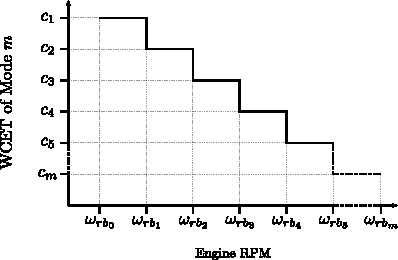
\includegraphics[scale=2.0]{fig/wcetVsRPM.pdf}
\caption{Adaptive Variable Rate (AVR) Task WCET versus Engine Speed}Different modes of an AVR task where $c_i$ and $\omega_{rb_i}$ are the execution time and the right boundary speed of the $i^{\rm th}$ mode, respectively.
\label{fig:AVRImage}
\end{figure}

Several methods have been proposed to calculate the \dbf~of an AVR task.
Mohaqeqi et al.~\cite{mohaqeqi_refinement_2017} proposed an exact analysis, using the Digraph model~\cite{stigge_digraph_2011}, to transform an AVR task into a digraph to calculate the exact worst-case demand assuming that the crankshaft can have multiple acceleration values during a rotation.
While this approach represents the state-of-the-art technique, it is computationally intensive and unlikely to be suitable for large problem instances.
In this paper, we propose a knapsack-based method to efficiently calculate the exact worst-case demand of an AVR task.

\noindent \textbf{Contributions}: The main contributions of this paper are:
\begin{enumerate}
\item To determine the worst-case demand of an AVR task, the search for the dominant job sequence, i.e., one that results in the maximum demand over a given time interval, is modeled as a bounded precedence constraint knapsack problem.
A dynamic programming based approach is presented to exactly and efficiently solve the problem.
\item  The number of job sequences that need to be considered when calculating the worst-case demand of an AVR task is significantly reduced by exploiting the kinematic properties of the engine.
\item Experimental results based on existing AVR task sets as well as randomly generated AVR task sets reveal that the proposed approach significantly outperforms the state-of-the-art technique~\cite{mohaqeqi_refinement_2017} in terms of computation time.
\end{enumerate}

The rest of the paper is organized as follows.
In Section~\ref{sec:prelims}, we introduce the system model, discuss our assumptions and formally present the problem.
In Section~\ref{sec:knapsack}, we present a knapsack-based approach to find the worst-case demand of AVR tasks. %...using the aforementioned dominant sequence set.
We provide some necessary conditions to reduce the search space in Section~\ref{sec:filterSeq} and describe the dominant sequence set in Section~\ref{sec:Summary}.
Experimental results are presented in Section~\ref{sec:experimental} and the paper concludes in Section~\ref{sec:conclusion}.
Note that related work was previously covered in Chapter \ref{chap:relatedWork}.

\subsection{Preliminaries}
\label{sec:prelims}

In this section, we provide some background materials on the engine and its properties and introduce our task model.
We also formally define the problem.
\paragraph{Task Model}
Adaptive variable rate (AVR) tasks are triggered at certain angles with respect to the top dead center position of the crankshaft, unlike periodic tasks which release jobs at regular time intervals.
For example, consider the different stages of fuel ignition in a vehicle as shown in Fig.~\ref{fig:Engine}.
For optimal performance of the engine, fuel injection should occur at a precise angle.
As the rate of arrival of the crankshaft at a given angle varies with its angular speed, AVR tasks do not have a fixed period.
Rather, at a higher speed, a larger number of instances (i.e., jobs) of each task occur, potentially increasing the resource requirement.

While it is possible to determine the schedulability of a task set assuming that this increased resource requirement of an AVR task is its steady-state demand, doing so would lead to pessimistic analyses and hence resource underutilization.
Moreover, the engine is more stable at higher speeds~\cite{dbuttle_real-time_nodate}.
This allows jobs to have shorter execution times at higher crankshaft speeds.
Hence, the execution time of AVR tasks is modeled as a function of the speed at which the jobs are released, as shown in Fig.~\ref{fig:AVRImage}.

%PNG Graphic
%\begin{figure}
%\centering
%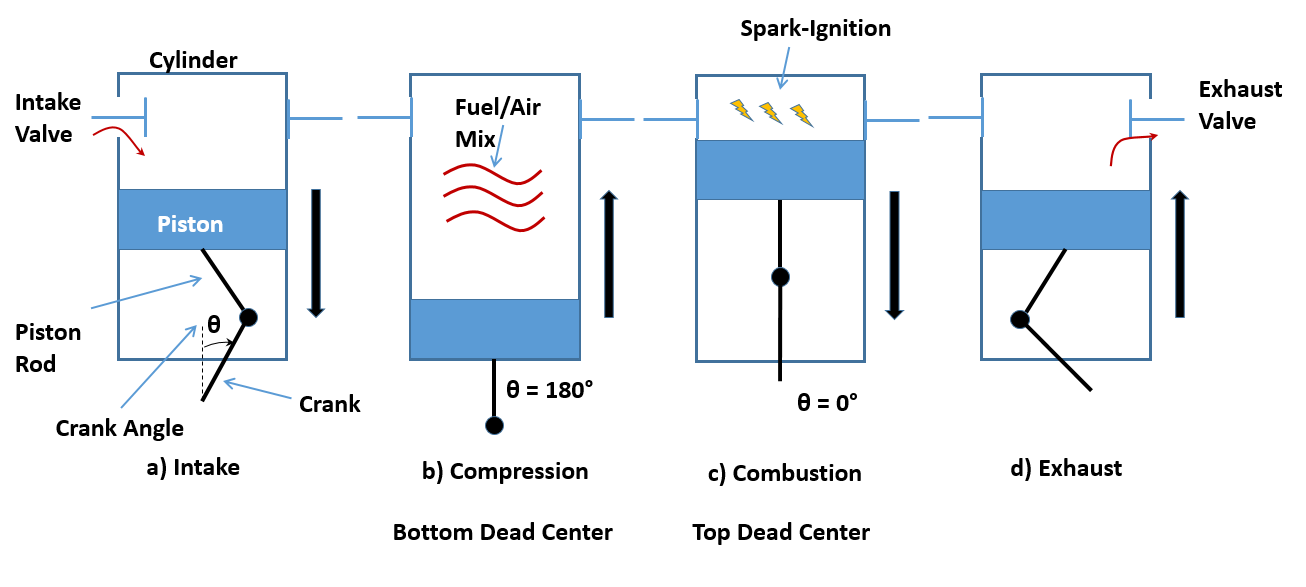
\includegraphics[width=\linewidth]{fig/Engine.PNG}
%\caption{Different stages of fuel ignition in a vehicle.}
%\label{fig:Engine}
%\end{figure}

%Vector Graphic - Last Update: 2018-08-21-12:05 - Aaron
\begin{figure}
    \centering
    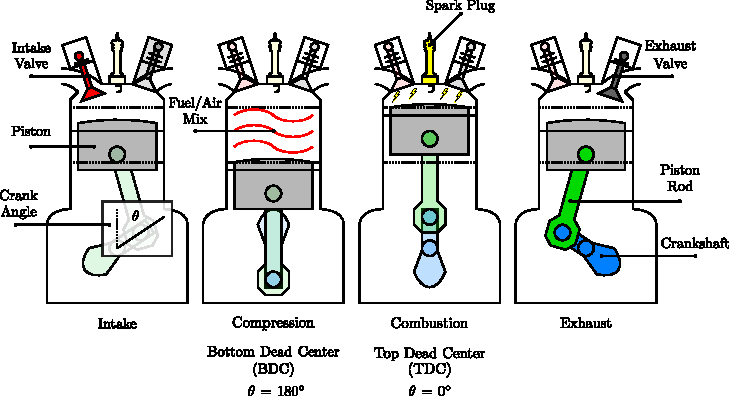
\includegraphics[width=0.9\linewidth]{fig/combustionCycle-4step.pdf}
    \caption{Stages of Ignition a Spark Ignition Internal Combustion Engine (ICE)}
    \label{fig:Engine}
\end{figure}

%An AVR task is typically modeled as a decreasing staircase function as shown in Fig.~\ref{fig:AVRImage}. 
The range of speeds in which the execution time is constant is referred to as a mode and the edge speeds of the mode are referred to as the \emph{boundary speeds} of the mode.
The set of speeds where the mode changes are defined as the set of right boundary speeds, i.e., $\mathbf{\Omega_{rb}}=\{\omega_{rb_1}, \ldots, \omega_{rb_{m}} \}$, 
$\forall \omega \in (\omega_{rb_{i-1}},\omega_{rb_i}]$, speed $\omega$ is in the $i^{\rm th}$ mode. 
%The right boundary speed of the $i^{\rm th}$ mode is represented as \(\omega_{rb_i}\).   
We further define $\mathbf{\Omega_{rb}}(\omega)$ to be all the right boundary speeds larger than $\omega$ that are reachable (defined later in Section~\ref{sec:prelims}). 
%As the staircase function is made of a series of steps, we use the terms steps and modes interchangeably. 
%\sandeep{If we don't use steps , we can remove this.}
The minimum and maximum allowable speeds of rotation of the crankshaft are represented by \(\omega_{rb_0}\) and \(\omega_{rb_m}\) respectively.
 For convenience, we refer to %these special right boundary speeds 
them as $\omega_{\min}$ and $\omega_{\max}$, respectively and assume $\omega \geq 0, \, \forall \omega \in [\omega_{\min},\omega_{\max}]$, where $\omega$ is assumed to be in $\text{rev/min}$.
In addition, the instantaneous speed at a given time $t$ is denoted as $\omega(t)$. %Alternatively, we also use the notation $\omega_\ell$ to represent the crankshaft speed at time $t_\ell$.
A table of notations can be found in Appendix \ref{appendix:engCtrl-table-of-notation}.

The maximum allowable acceleration and deceleration are denoted by \(\alpha_{\max}\) and \(\alpha_{\min}\), respectively, both assumed to be in $\text{rev/min}^2$.
In this paper, we assume $\alpha_{max}=|\alpha_{min}|$.
The execution time of the $i^{\rm th}$ mode is represented by $c_i$.
Additionally, the execution time corresponding to a speed $\omega(t)$, is denoted by $c(\omega(t))$.
We assume that a job is released at the top dead center position, which we consider as the beginning of the rotation.
Thus, a job's execution time is determined by the speed of the crankshaft at the beginning of its the rotation.

\begin{property}[Speed After $n$ Rotations]
Given an initial speed of $\omega(t)$ at time $t$ and a constant acceleration $\alpha$,
the speed after an angular displacement of $\Delta \theta$
is~\cite{verma_concepts_nodate, biondi_exact_2014}
\begin{equation}
\label{eqn:rotation}
    \Omega(\omega(t),\alpha, \Delta \theta) = \sqrt[]{\omega(t)^2+2\alpha \Delta \theta}.
\end{equation}

Similar to the work by Mohaqeqi et al.~\cite{mohaqeqi_refinement_2017} we assume that $\Delta \theta$ specifies the crankshaft revolution in terms of the number of rotations, i.e., $ \Delta \theta = 1$ indicates a complete rotation.
Hence, according to Equation~\ref{eqn:rotation}, assuming an initial speed of $\omega(t)$ at time $t$, and a constant acceleration of $\alpha$, the speed after one complete rotation is $\Omega_1(\omega(t),\alpha) = \sqrt[]{\omega(t)^2+2\alpha}$.
In general, the speed after $n$ complete rotations is~\cite{mohaqeqi_refinement_2017},
\begin{equation}
\label{eqn:rotation-n}
    \Omega_n(\omega(t),\alpha) = \sqrt[]{\omega(t)^2+2 n \alpha}.
\end{equation}
\end{property}


Biondi et al. \cite{biondi_response-time_2015} showed that multiple AVR tasks activated by the same source and, which have the same angular phase and period can be modeled as a single AVR task, called the representative AVR task.
Hence, the analysis in this paper can also be extended to multiple AVR tasks.


\paragraph{Minimum Job Inter-arrival Times}

The minimum inter-arrival time is the minimum time duration from the release of a job at $t_1$ when the speed is $\omega(t_1)$ to the next job release at $t_2$ and speed $\omega(t_2)$. We denote minimum inter-arrival time by $\widetilde{T}(\omega(t_1),\omega(t_2))$.
In order to overcome the drawback of using constant acceleration between job releases as was assumed in most existing work~\cite{biondi_response-time_2015,biondi_feasibility_2015,biondi_exact_2014}, we consider the possibility of acceleration variations between two job releases similar to the work by Mohaqeqi et al.~\cite{mohaqeqi_refinement_2017}.

The minimum inter-arrival time equation by Mohaqeqi et al.~\cite{mohaqeqi_refinement_2017} is briefly presented here using simplified notation for readability.
To get the minimum inter-arrival time from any speed $\omega$, the crankshaft has to be maximally accelerated from $\omega$ to reach $\omega_{p}$, the peak speed, and then maximally decelerated to reach a target speed $f$ in a single rotation,
% \begin{equation}\label{eq:peakSpeed}
% \omega_{peak} = \sqrt{\frac{2\alpha_{\min}\alpha_{\max}+\alpha_{\min}\omega(t_1)^2-\alpha_{\max}\omega(t_2)^2}{\alpha_{\min} - \alpha_{\max}}}.
% \end{equation}
\begin{equation}\label{eq:peakSpeed}
\omega_p(\omega,f) = \frac{\sqrt{2\omega^2 + 2f^2 + 2\alpha_{\max}}}{2}.
\end{equation}

However, if $\omega_{p}>\omega_{max}$, the crankshaft has to maximally accelerate from $\omega$ to $\omega_{max}$, stay at that speed for some time and then maximally decelerate to $f$.
The two cases are defined below and presented in Figure \ref{fig:mint}:
% \begin{alignat}{3}\label{minTime}
%     &\widetilde{T}(\omega(t_2),\omega(t_1)) = \nonumber &\\
%     &\left\{
%         \def\arraystretch{2.0} %Switch to 2.2 for best results
%         \begin{array}{ll}
%             \frac{\omega_{rb_m}-\omega(t_1)}{\alpha_{max}} 
%             + \frac{\omega(t_2) - \omega_{rb_m}}{\alpha_{min}} +\frac{1}{\omega_{rb_m}} \cdot \\ \bigg(1-\frac{\omega_{rb_m}^2-\omega(t_1)^2}{2\alpha_{max}}           -\frac{\omega(t_2)^2-\omega_{rb_m}^2}{2\alpha_{min}} \bigg)
%             & \omega_{peak} > \omega_{\max} \\
%             \frac{\omega_{peak}-\omega(t_1)}{\alpha_{\max}} + \frac{\omega(t_2)-\omega_{peak}}{\alpha_{\min}} & \omega_{peak} \leq \omega_{\max}
%         \end{array}
%     \right.
% \end{alignat}
\begin{alignat}{3}\label{eq:minTime}
  &\widetilde{T}(\omega,f) = \\
  &\left\{
        \def\arraystretch{2.0}
        \begin{array}{ll}
            \frac{\sqrt{2\omega^2+2f^2+4\alpha_{\max}}-\omega-f}{\alpha_{\max}} & \ \omega_p(w,f) \leq \omega_{\max} \ \\
            \frac{\omega_{max} - f - \omega}{\alpha_{\max}} + \frac{\omega^2 + f^2}{2\omega_{\max}\alpha_{\max}}+\frac{1}{\omega_{\max}} & \ \omega_p(w,f) > \omega_{\max}
        \end{array}
    \right. \nonumber
\end{alignat}

\begin{figure}
\centering
  \subfloat[$\widetilde{T}(\omega,f) | \omega_{p}(\omega,f) \leq \omega_{\max}$]{
      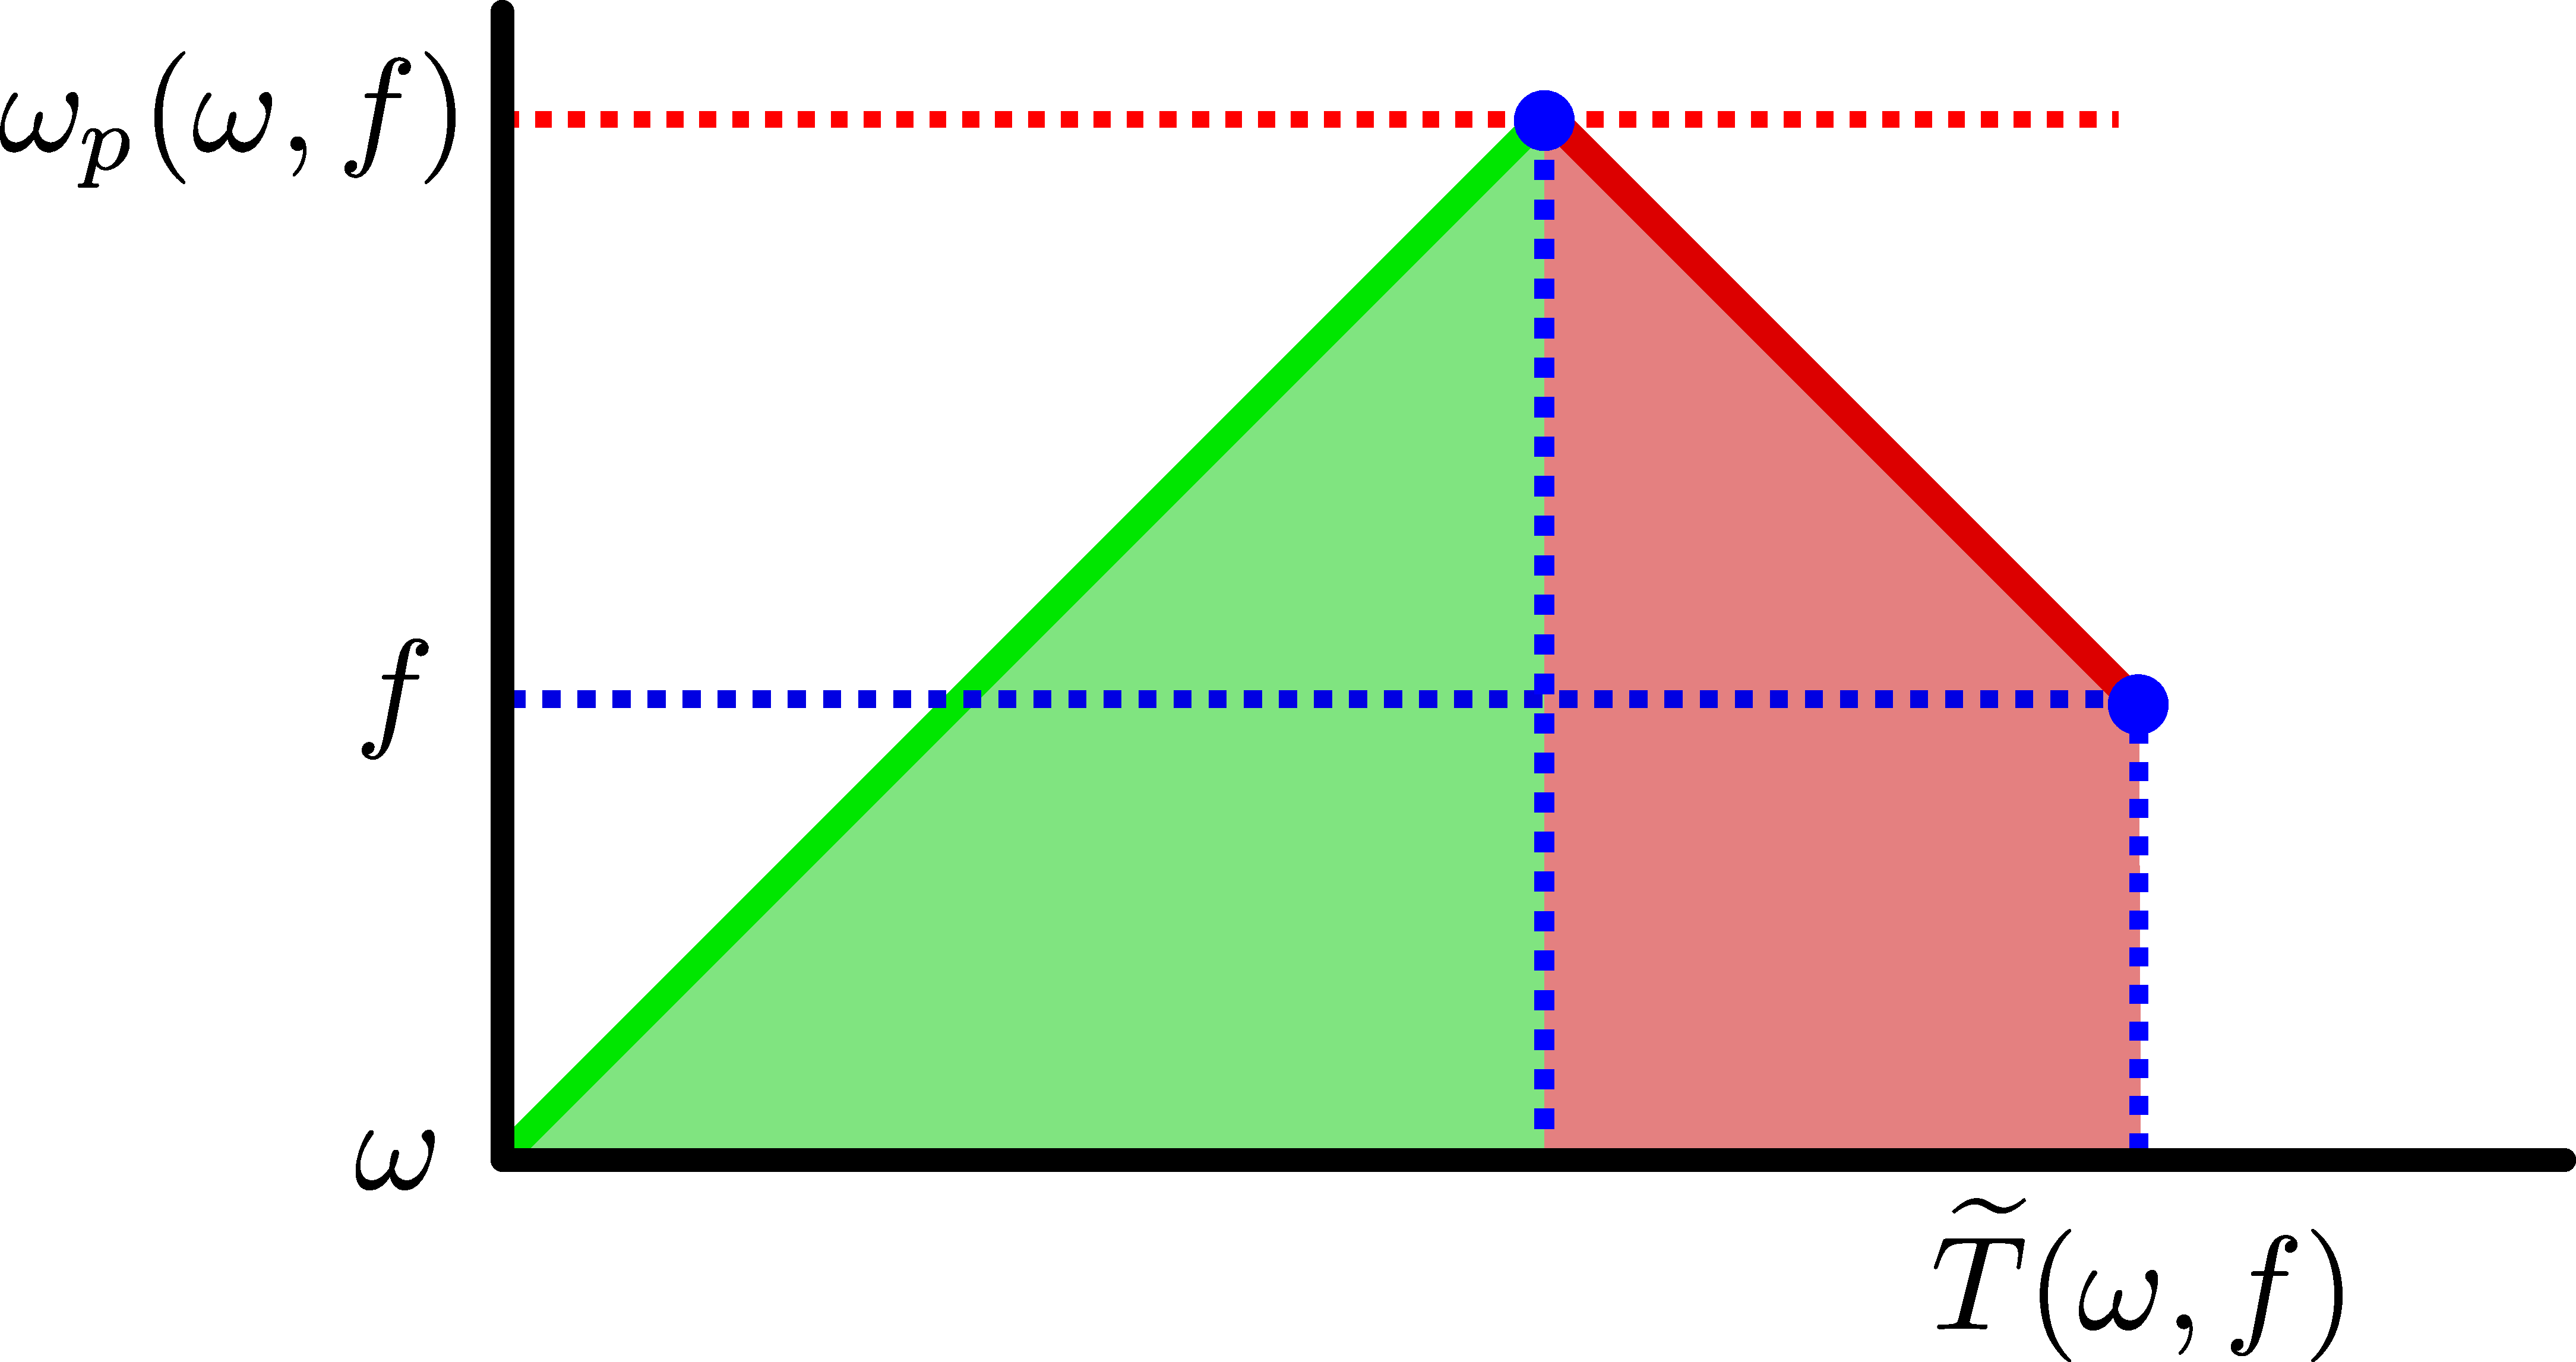
\includegraphics[scale=0.1]{fig/mint-peakBare.pdf}}
      \label{fig:mintPeak}
  \label{mintPeak}
  \subfloat[$\widetilde{T}(\omega,f) | \omega_{p}(\omega,f) > \omega_{\max}$]{
      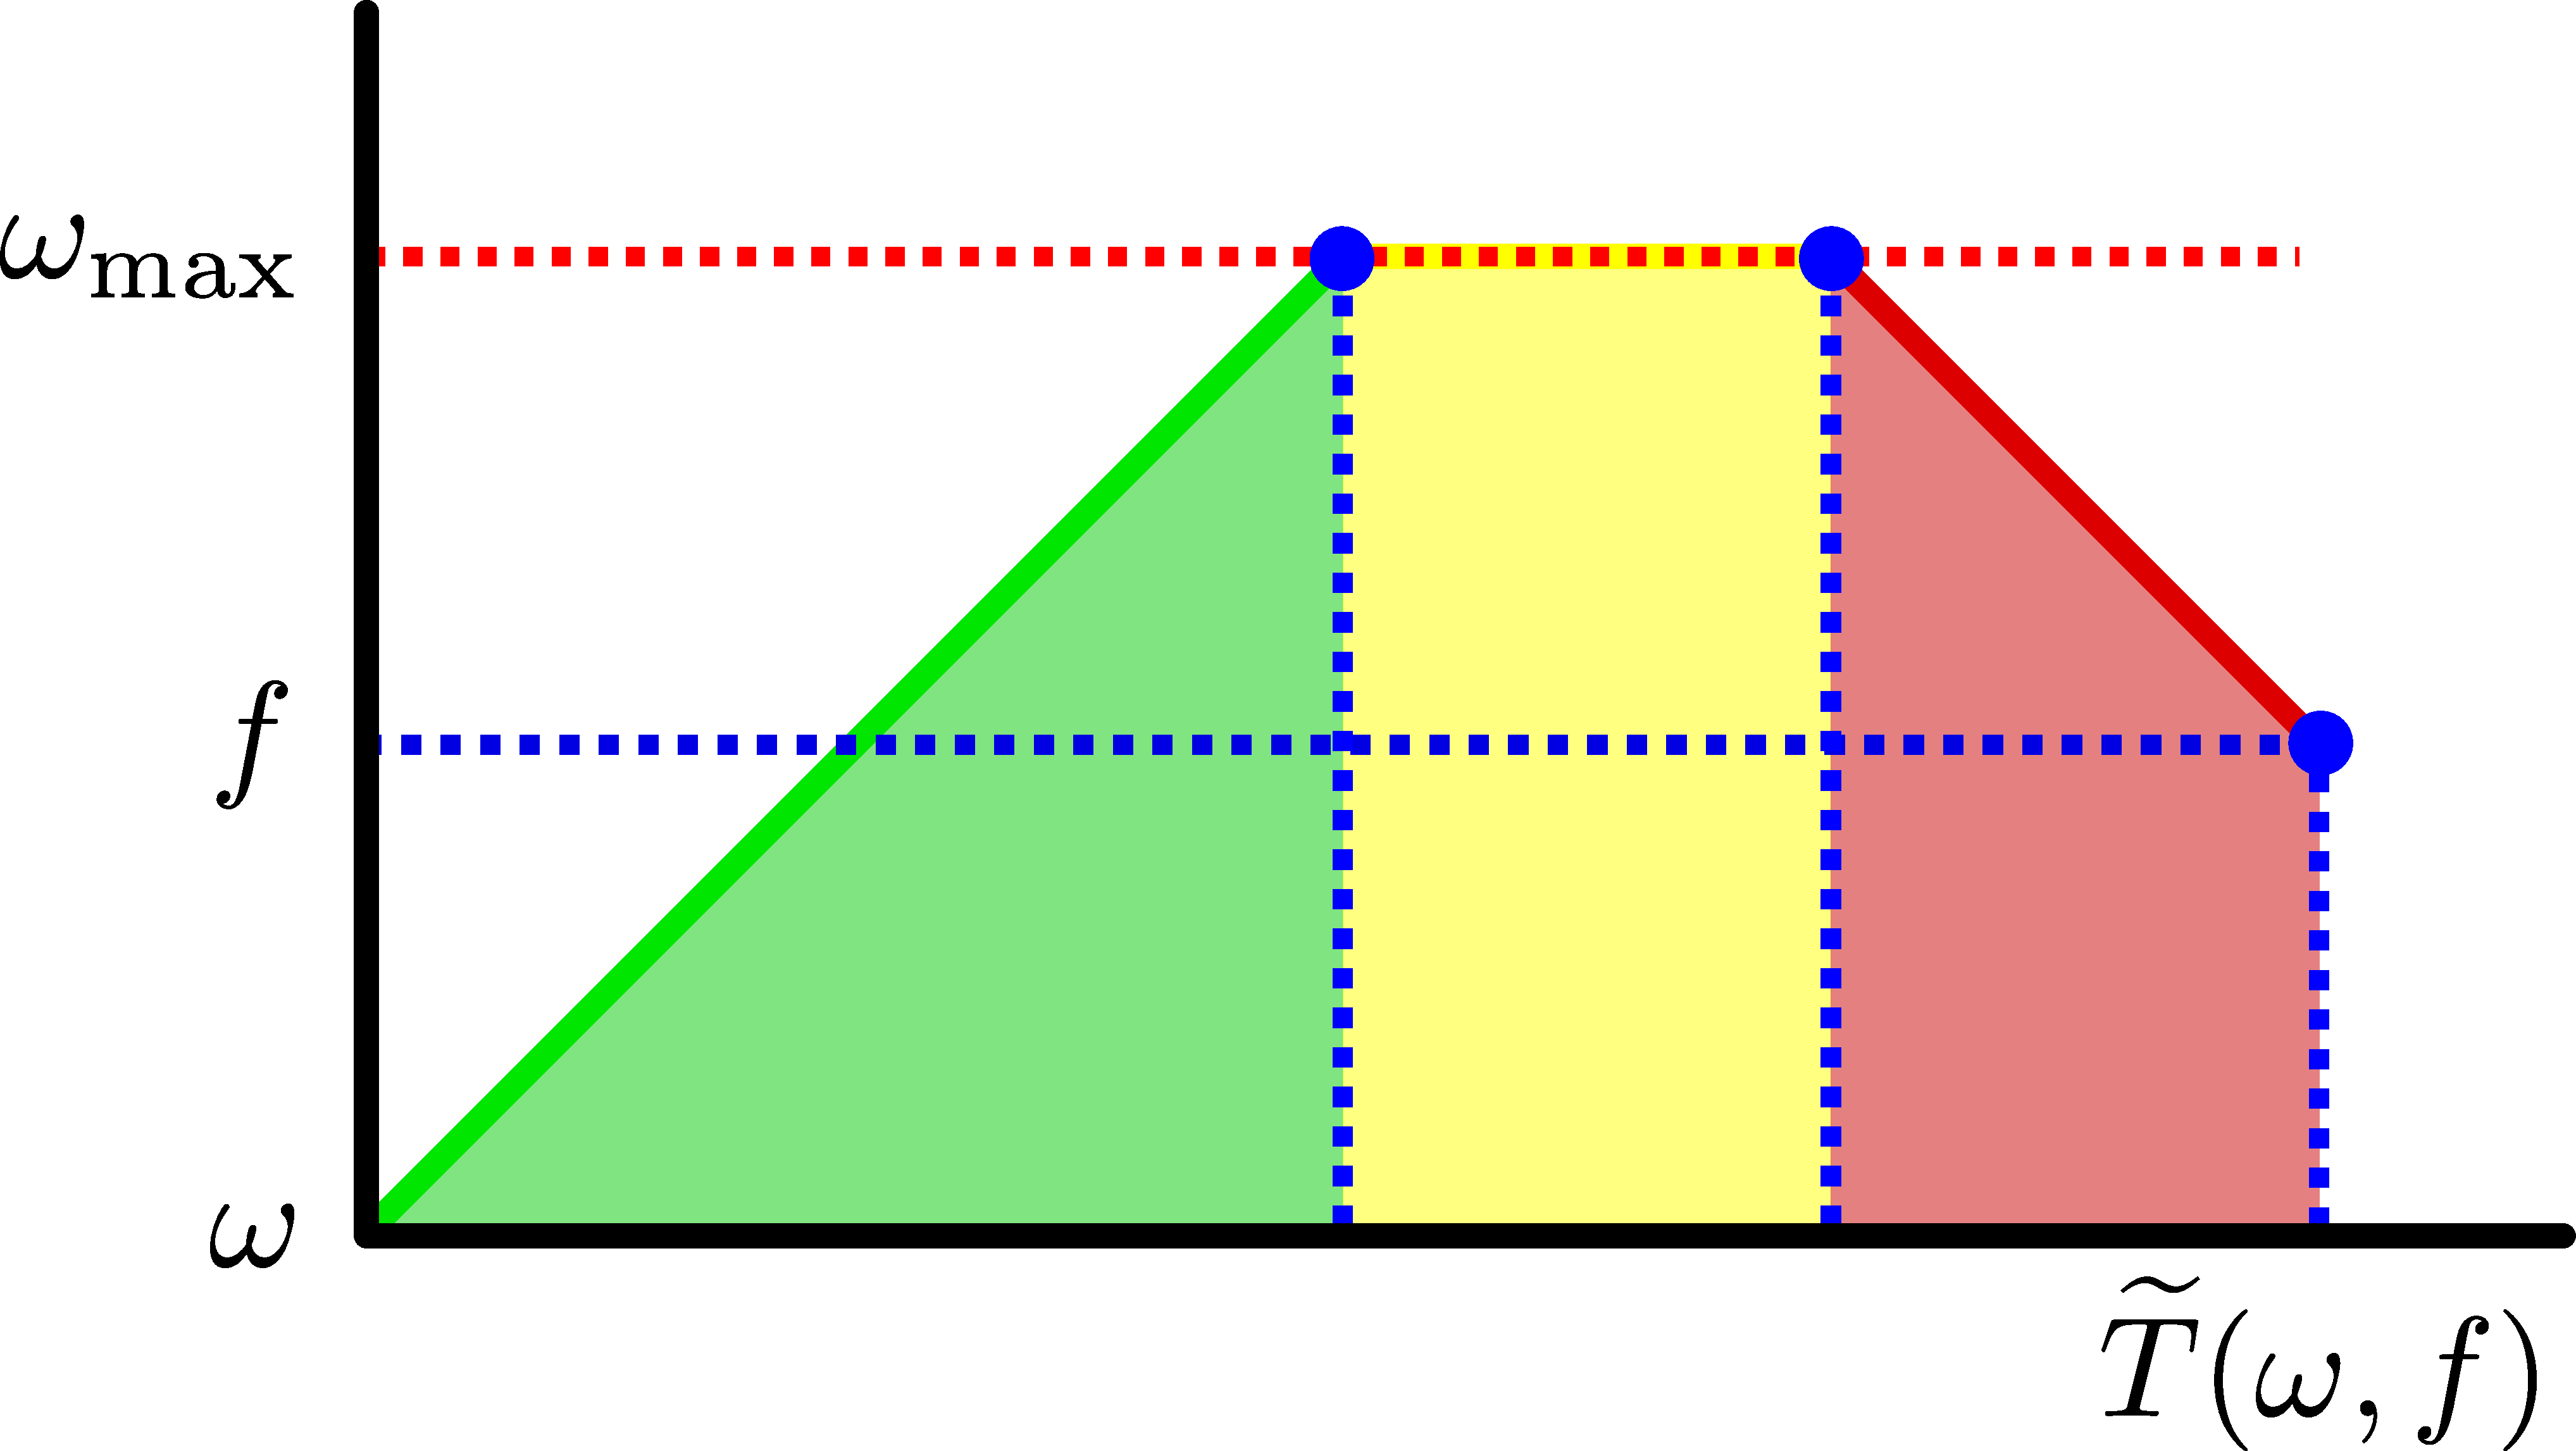
\includegraphics[scale=0.1]{fig/mint-limitBare.pdf}}
      \label{fig:mintMax}
  \label{mintMax}
%\caption{Minimum interarrival time $\widetilde{T}(\omega,f)$ between speeds $\omega$ and $f$ where (a) $\omega_p(\omega,f) \leq \omega_{\max}$ and (b) $\omega_p(\omega,f) > \omega_{\max}$. Green, ascending lines represent periods of maximum acceleration, $\alpha_{\max}$, yellow, flat lines represent periods of zero acceleration, $\alpha = 0$, and red, descending lines represent periods of maximum deceleration, $\alpha_{\min}$.}
\caption{Minimum Interarrival Time Graphs: With and Without $\omega_{max}$}Minimum interarrival time $\widetilde{T}(\omega,f)$ between speeds $\omega$ and $f$ where (a) $\omega_p(\omega,f) \leq \omega_{\max}$ and (b) $\omega_p(\omega,f) > \omega_{\max}$.
Ascending, flat, and descending lines represent periods of maximum ($\alpha_{\max}$), zero, and  minimum ($\alpha_{\min}$) acceleration, respectively.
\label{fig:mint}
\end{figure}

\begin{property}[Reversability of Inter-Arrival Times]
\label{T-reversal}
$\widetilde{T}(\omega(t_1),\omega(t_2)) = \widetilde{T}(\omega(t_2),\omega(t_1))$.
In other words, the minimum inter-arrival time from a job released at $\omega(t_1)$ to a job released at $\omega(t_2)$ is equal to the inter-arrival time when the speeds are in the reverse order.
\end{property} 


\paragraph{AVR Task Demand}
Let $\mathbb{W}$ be the set of all possible speed functions $\omega(t)$ that are feasible (i.e., $\omega(t)$ is any continuous function with acceleration between $\alpha_{\min}$ and $\alpha_{\max}$ and speeds between $\omega_{\min}$ and $\omega_{\max}$).
 For any such $\omega(t)$, considering that a computational job of an AVR task is released at time $t'$, we assume that the processor must successfully complete execution of this job by time $t' + \widetilde{T}(\omega(t'), \min(\Omega_1(\omega(t'), \alpha_{\max}),\omega_{max}))$; that is, the absolute deadline of this job coincides with the minimum time to complete a single rotation from a given speed $\omega(t')$. 
% \aaron{Is this deadline assumption problematic? We claim to use implicit deadline but the above implies that any non-maximally accelerated task would be constrained deadline. Thoughts?} 
We refer to an AVR task that sets deadlines in this way as a {\bf minimum angular deadline AVR task}~\cite{biondi_modeling_2018} and refer to the relative deadline of a job released at speed $\omega$ as 
%{\bf minimum relative deadline}, 
$\tilde{d}(\omega) = \widetilde{T}(\omega(t'), \min(\Omega_1(\omega(t'), \alpha_{\max}),\omega_{max}))$.
We may denote the {\em demand} of $\omega(t)$ over any $\delta$-length interval $[t_a, t_b]$ as $D_{\omega(t)}(t_a, t_b)$.
 $D_{\omega(t)}(t_a, t_b)$ represents the total execution requirement of jobs released by the speed function with both arrival times and absolute deadline in the interval $[t_a, t_b]$.
 More formally, if $\{t_1, t_2, \ldots\}$ is the set of times (in order) where the crankshaft triggers job releases following the speed function $\omega(t)$, then:
\begin{equation}
\label{eqn:d}
    D_{\omega(t)}(t_a, t_b) = \hspace{-.2in}\sum_{i: (t_i \geq t_a) 
            \wedge (t_i +\tilde{d}(\omega(t_i)) \leq t_b)}   \hspace{-.2in} c(\omega(t_i)).
\end{equation}

\noindent We can compute the upper envelope on the demand over any interval of length $\delta > 0$ for $\omega(t)$ as:
\begin{equation}\label{eqn:speed-fn-dbf}
    \dbf_{\omega(t)}(\delta) = \max_{t' \geq 0} \{D_{\omega(t)}(t', t' + \delta)\}.
\end{equation}

\noindent The \emph{worst-case demand} of an AVR task over any $\delta$-length interval is the speed schedule that maximizes the value of the upper envelope given in Equation~\ref{eqn:speed-fn-dbf}:
\begin{equation}\label{eqn:AVR-dbf}
    \dbf(\delta) = \max_{\omega(t) \in \mathbb{W}} \{\dbf_{\omega(t)}(\delta)\}.
\end{equation}
Considering any speed function $\omega(t)$ with job releases at speeds/times $\omega(t_1),\omega(t_2),\ldots$ in some interval $[t_a, t_b]$, it is clear that if we modify the function so that the crankshaft traverses one rotation in the minimum time (by Equation~\ref{eq:minTime}), then this will only lead to demand that exceeds or equals the original demand of $\omega(t)$.
Therefore, without loss of generality, we can restrict $\mathbb{W}$ to speed functions that traverse the rotation between job releases in the minimum possible time.
 This is essentially the observation made by Mohaqeqi et al.~\cite{mohaqeqi_refinement_2017} to reduce the problem of finding the worst-case $\omega(t) \in \mathbb{W}$ to the problem of identifying \emph{sequences of job release speeds}; i.e., the speed of the job releases entirely characterizes the speed function.
That is, we can completely describe any speed function $\omega(t)$ with job releases at times $t_1, t_2, \ldots$ instead by a sequence of speeds $(\omega_1 = \omega(t_1), \omega_2 = \omega(t_2), \ldots)$.
 Thus, after this point, we drop the speed-time function $\omega(t)$ and focus only on sequences of speeds.

\noindent The objective of this paper is to find an efficient way to calculate the worst-case AVR task demand defined in Equation~\ref{eqn:AVR-dbf}.

\begin{definition}[Reachable Speeds]\label{def:reachable-speeds}
Consider two speeds $\omega_1$ and $\omega_2$ such that $\omega_2\geq\omega_1$.
$\omega_2$ is said to be \emph{reachable} from $\omega_1$ if $\Omega_1(\omega_1,\alpha_{max})\geq \omega_2$.
\end{definition}

\begin{definition}[Valid Sequence]\label{def:valid-sequence}
A set of jobs ${j_1,j_2,j_3,\ldots,j_k}$ released at speeds $\omega_1,\omega_2,\ldots,\omega_k$ is said to be a valid sequence of speeds if 
%Original footnote
%$\forall i \in \mathbb{N}^k_2\footnote{$\mathbb{N}^k_j$ represents the set $\{j,j+1,\ldots,k\}$},\,\omega_i$ is reachable from $\omega_{i-1}$.
$\forall i \in \mathbb{N}^k_2$, $\omega_i$ is reachable from $\omega_{i-1}$ where $\mathbb{N}^k_j$ is the set of natural numbers from \textit{j} to \textit{k}, i.e., $\{j,j+1,\ldots,k\}$.
%$\forall i \in \{2,\ldots,n\},\, \Omega(\omega(t_i),\alpha_{min}))\geq \omega(t_{\mathit{i-1}})$ and $\forall i \in \{1,\ldots,n-1\},\, \Omega(\omega(t_i),\alpha_{max}))\leq \omega(t_{\mathit{i+1}})$. 
%and $\Omega(\omega(t_2),\alpha_{min})\geq\omega(t_1)$ 
\end{definition}
\paragraph{Problem Definition} 
%Potentially there can be infinite sequences of jobs released depending on the instantaneous angular speed and angular acceleration of the crankshaft. 
Consider a minimum angular deadline AVR task, which is characterized by feasible speed $\left[\omega_{\min}, \omega_{\max}\right]$ and acceleration $\left[\alpha_{min}, \alpha_{max}\right]$ ranges, where $\alpha_{max} = |\alpha_{min}|$, and a set of modes $\mathbf{\Omega_{rb}}=\{\omega_{rb_1}, \ldots, \omega_{rb_m} \}$, each of which is associated with an execution time $c(\omega_{rb_i})$, $i = 1, \ldots, m$, as discussed earlier in this section.
The objective is to find $\dbf(\delta)$ (Equation~\ref{eqn:AVR-dbf}), the worst-case demand of the AVR task over any $\delta$-length interval $[t_a, t_b]$ assuming that the acceleration of the crankshaft may change within a single rotation.

\subsection{Knapsack-based approach for deriving the worst-case demand}
\label{sec:knapsack}

We now describe the problem transformation from calculating $\dbf(\delta)$ to a variant of the knapsack problem.
This section both provides context for and relies upon several  properties and  lemmas defined in Sections \ref{sec:filterSeq} and \ref{sec:Summary}.
Briefly, \textit{dominant speed sequences} are sequences of job release speeds whose demand %is equivalent to the maximum demand of a task over a given interval length (i.e., the demand of a dominant speed sequence 
coincides with the value of Equation \ref{eqn:AVR-dbf}.
These dominant speed sequences are non-decreasing (see Section \ref{subsec:seq-transform}, Lemma \ref{lemma:non-decreasing}) and start at right boundary speeds (see Section \ref{sec:dominant-start}, Lemma \ref{lemma:startSpeed}).

% {\color{blue}Add a paragraph outlining what to expect later. Aaron: Is the above sufficient?}
% \sandeep{I think we will need to explain about the items in the knapsack too. In the 2nd and 3rd paragraphs from here, we explain about the dependency of the items in the knapsack. I think this will be challenging to do without actually giving the proofs.}
% \aaron{I believe this is already done. See paragraph immediately following.}
% \sandeep{We do not explain about the limited numbers of jobs following a given job and about the sequence only being non-decreasing. One way to do this is just note all the constraints on the sequences we prove later and say that for proof please refer to later sections.}

In the traditional knapsack problem, the aim is to maximize the total profit from a given set of items where each item is associated with a profit and weight, while ensuring that the aggregate weight is less than or equal to the maximum allowable weight of the knapsack.
Our goal is to transform the problem of finding $\dbf(\delta)$ into a variant of the knapsack problem.
In our case, a job is equivalent to an item.
%and is characterized by: the speed at the beginning of the rotation, the corresponding execution time, and the minimum inter-arrival time given the speed at the beginning of the rotation (Equation~\ref{eq:minTime}) -- which depends on the initial speed of the subsequent job.
As such, the ``weight" of a job (i.e., item) is the minimum inter-arrival time, and the ``profit" is its execution time.
The goal, then, is to maximize demand (i.e., profit) over a time interval ($\delta$).

Since a dominant speed sequence is non-decreasing (Lemma~\ref{lemma:non-decreasing}), a job's execution time may contribute to the demand bound function $\dbf(\delta)$ more than once.
As such, our knapsack problem is, in fact, a bounded knapsack problem.
In addition, since  adjacent speeds in a dominant speed sequence must be reachable from one another (Definition \ref{def:reachable-speeds}), once an item, i.e., job, has been included in the knapsack, there is a finite number of jobs that can follow, making our problem a bounded precedence constraint knapsack problem (BPCKP)~\cite{cho_depth-first_1997,johnson_knapsacks_1983}.
Fig.~\ref{fig:Knapsack1} provides a visual example representation of our problem as a BPCKP.
For clarity, the subscripts of the speeds are used to denote the precedence constraints.
\begin{figure}
\centering
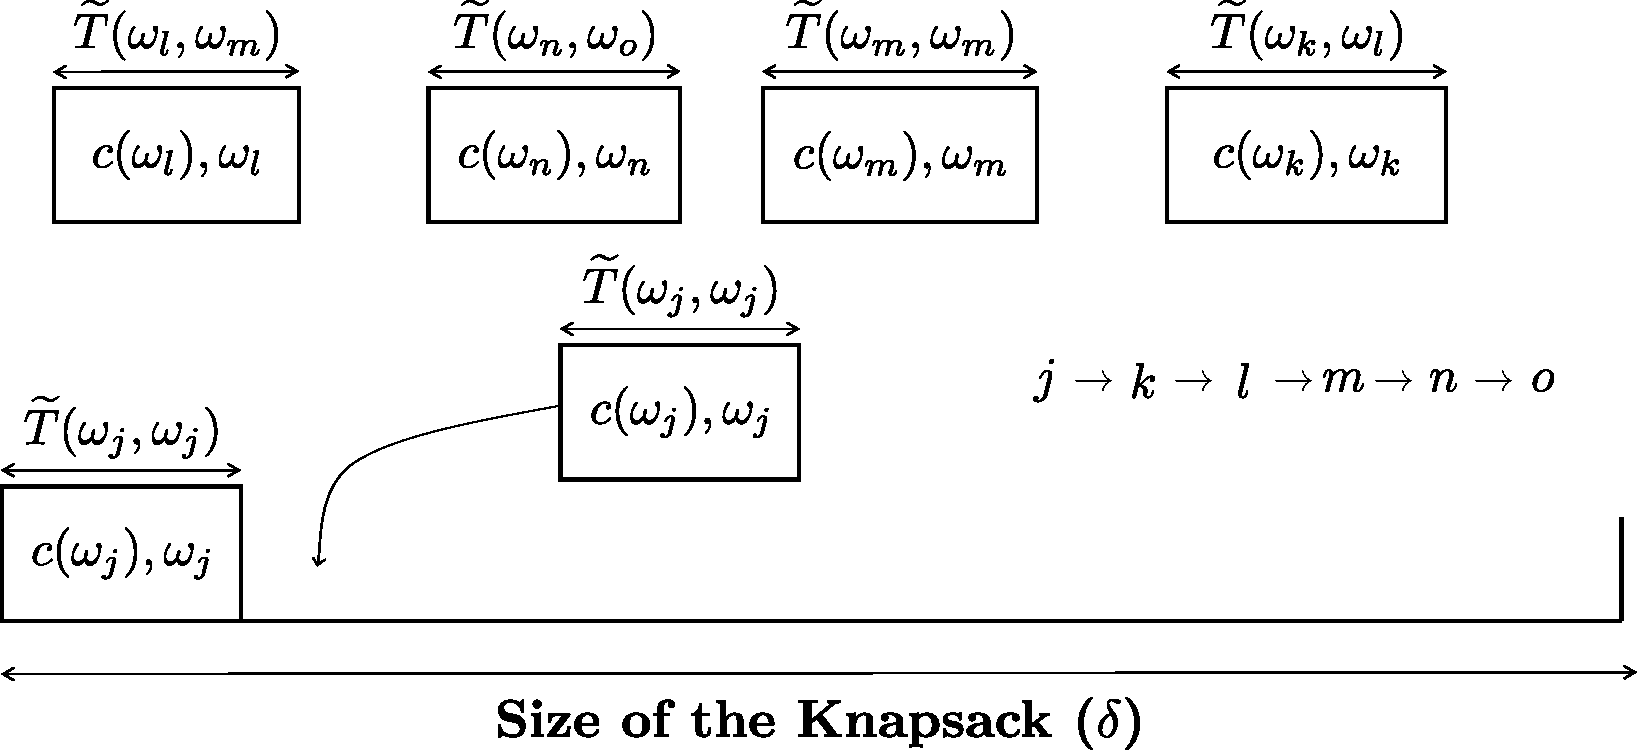
\includegraphics[width=1.0\linewidth]{fig/vectorKnapsackv2.pdf}
\caption{Example Knapsack Item Visualization} Example knapsack items for calculating worst case demand of an AVR task. A job that is higher in the precedence relation is preceded by a job lower in the relation.
\label{fig:Knapsack1}
\end{figure}

%PNG
%\begin{figure}
%\centering
%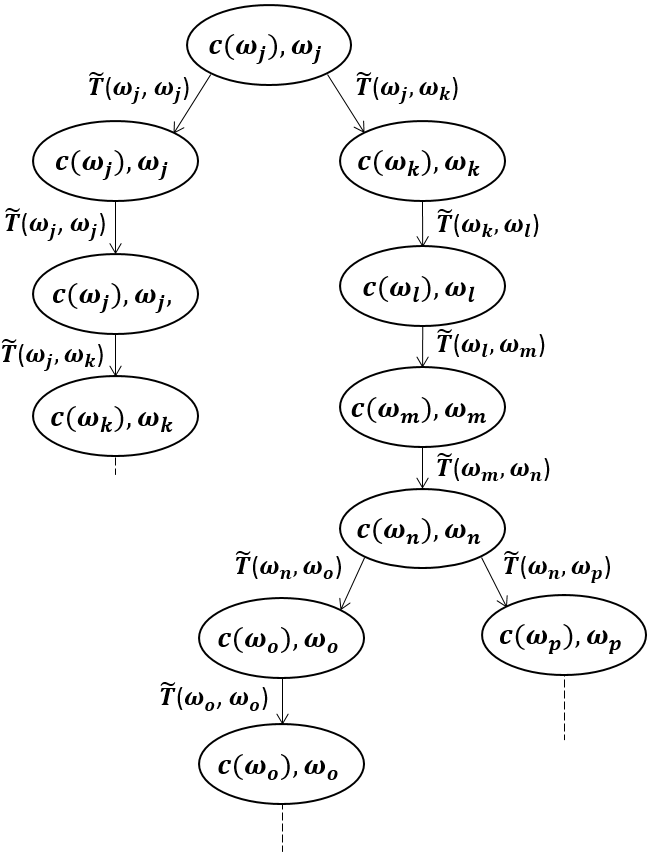
\includegraphics[width=0.5\linewidth]{fig/KnapsackTree.PNG}
%\caption{Precedence constraints among jobs are expressed using out-trees.}
%\label{fig:KnapsackTree}
%\end{figure}

%Vectorized Image
%\begin{figure}
%    \centering
%    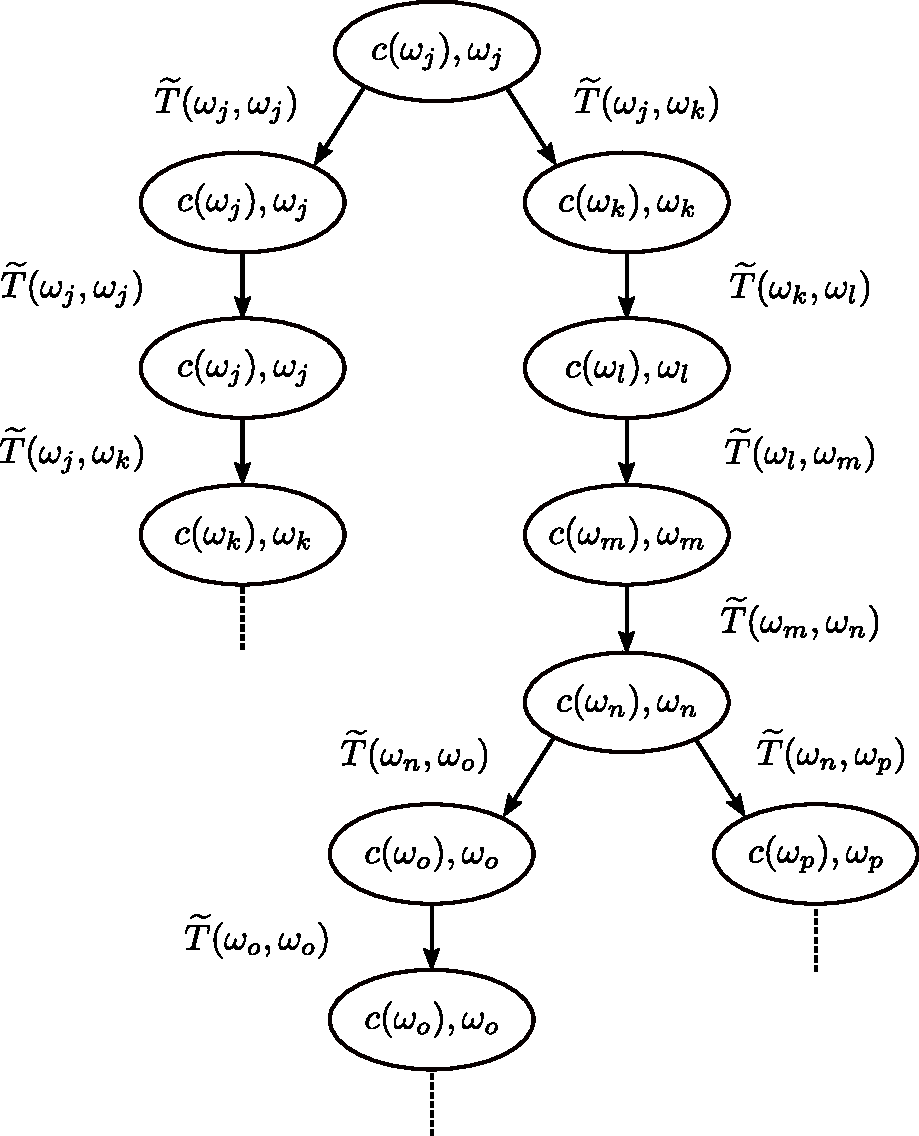
\includegraphics[width=0.8\linewidth]{fig/vectorKnapsackTreeIsolated.pdf}
%    \caption{Precedence constraints among jobs are expressed using out-trees.}
%    \label{fig:KnapsackTree}
%\end{figure}

%Vectorized, Shortened
\begin{figure}
    \centering
    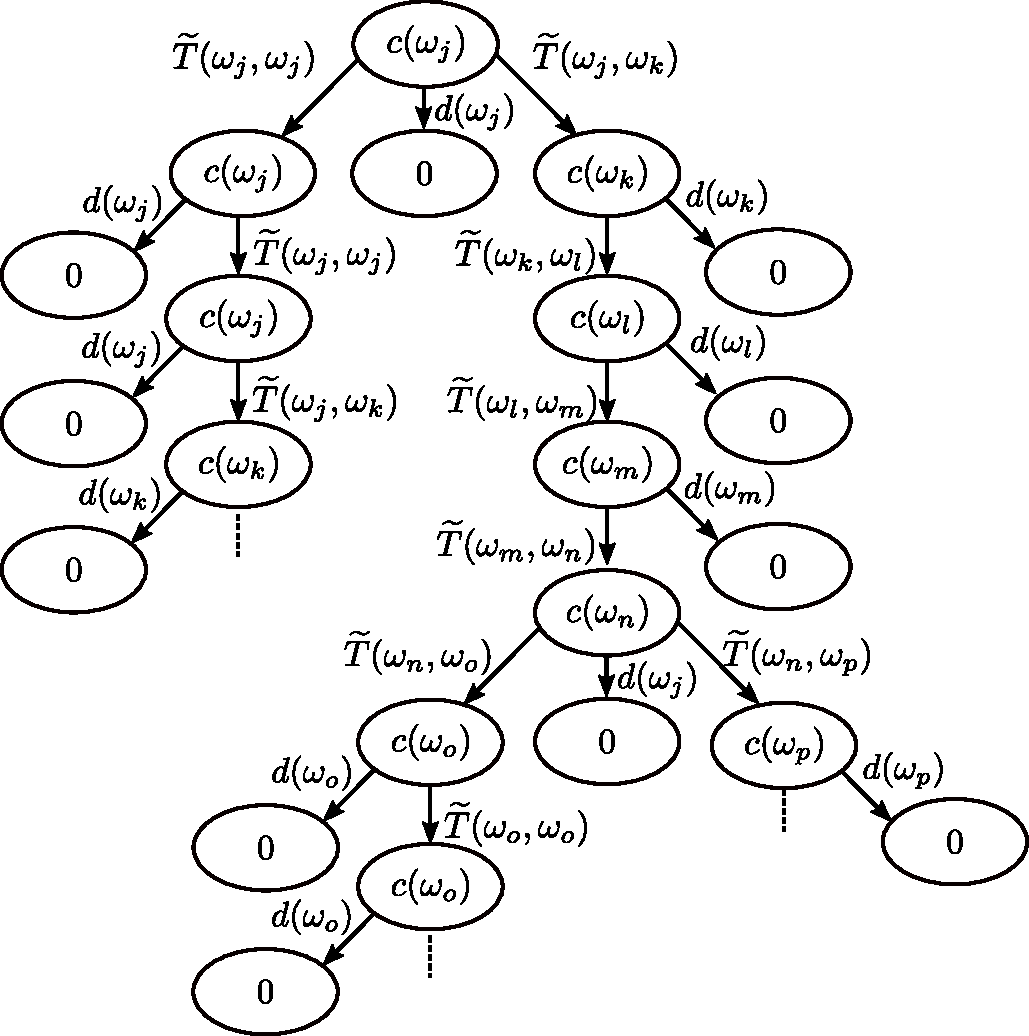
\includegraphics[width=1.0\linewidth]{fig/vectorKnapsackTreeShortenedv5.pdf}
    \caption{Example Out Tree of Knapsack Items}Precedence constraints among jobs are expressed using out-trees. Nodes represent WCETs for initial speeds and arrows represent minimum inter-arrival times. The tree demonstrates various precedence relations and possible paths. Leaves represent completion of the parent job without subsequent jobs (i.e. items). Each leaf has zero execution since its parent is the final job included in the knapsack.
    \label{fig:KnapsackTree}
\end{figure}

An effective way to model the precedence constraints among jobs is by using out-trees.
The sequences beginning at each of the source nodes are independent of each other (i.e., sequences beginning at each of the right boundary speeds according to Lemma~\ref{lemma:startSpeed}).
An example out-tree is shown in Fig. \ref{fig:KnapsackTree}.
To represent the trees in a knapsack problem, we define a dependency graph $G_I=(V_I, A_I)$, where $V_I$ denotes the set of vertices (i.e., items) in the out-tree $G_I$~\cite{kellerer_knapsack_2004}.
An edge between any two vertices denotes that the two speeds are reachable from one another and is represented by $(j,k)\in A_I$.
Formally, our BPCKP can be expressed as follows:
\begin{alignat}{3}
    & \underset{x}{\text{maximize}}
    & \quad & \sum_{j}\sum_{r=1}^{M_\delta} c(\omega_j) \cdot x_j^{r} \label{eqn:maxDemand}\\
    & \text{subject to}
    & \quad & \sum_{j, k | (j,k) \in A_I} \sum_{r=1}^{M_\delta}  \tilde{T}(w_j, w_k) \cdot x_k^r \leq \delta \label{eqn:kp-cons}\\
    & & \quad & \sum_{k|(j,k)\in A_I} x_k^1 \leq 1, \, \forall j \label{eqn:singleKnapsackPath}\\
    & & \quad & x_j^1 \geq x_k^1, \, \forall (j,k)\in A_I \label{eqn:precedenceConstraint}\\
    %& & \quad & m \in \{1,2,3,...,M_\delta\} %\label{eqn:mValueSet}\\
    % & & \quad & M = 1,2,.. \,\,\forall \omega_j \in \mathbf{\Omega_{rb}}\\
    % & & \quad & x_j^{\eta_j} \geq x_k^{\eta_k}, \,\, (j,k)\in A_I \label{eqn:kp-prec}\\
    %& & \quad & x_j^{m} \in \{0,1\} \\
    & & \quad & x_j^r \geq x_j^{r+1}, \,\, \forall j, r \in \{1,2,3,...,M_\delta-1\} \label{eqn:multipleJobRestriction}\\
     & & \quad &x_j^r \in \{0,1\},\,\forall j,  r \in \{1,2,3,...,M_\delta\} \label{eqn:binaryXValue}
    % & & \quad & \eta_j \in \mathbb{Z}^+ \,\, \forall \, x_j^{\eta_j} \, | \, \omega_j \in \mathbf{\Omega_{rb}} \label{eqn:eta-boundary-jobs}\\
    % & & \quad & \eta_j \in \{0,1\} \,\, \forall \, x_j^{\eta_j} \, | \, \omega_j \notin \mathbf{\Omega_{rb}} \label{eqn:eta-special-jobs}
\end{alignat}
%Original Eqn:
% \noindent maximize
% \begin{equation}
% \sum_{j=1}^{\infty}c(\omega_j) \cdot x_j^\eta
% \end{equation}
% \newline
% subject to
% \begin{equation}
% \label{eqn:kp-cons}
% \sum_{j=1}^{\infty}\widetilde{T}(\omega_j, \omega_k) \cdot x_j^\eta \leq \delta
% \end{equation}
% \begin{equation}\label{eq:kp3}
% x_j^\eta \geq x_k^\eta, \,\, (j,k)\epsilon A_I
% \end{equation}
\noindent where $M_\delta$ represents an upper bound on the number of job releases in a $\delta$-length interval and  $x_j^r$ is a binary variable: $x_j^r$ is one if there are at least $r$ jobs released at speed $\omega_j$ in the knapsack; otherwise, $x_j^r$ is zero.
Equation \ref{eqn:maxDemand}  maximizes total demand.
Equation \ref{eqn:kp-cons} requires all deadlines of selected jobs fall within the $\delta$-length interval.
Equation \ref{eqn:singleKnapsackPath} permits at most one child node of each parent node to be added to the knapsack.
Equation \ref{eqn:precedenceConstraint} enforces the precedence constraint such that no child node may be added without its parent.
Equation \ref{eqn:multipleJobRestriction} ensures repeated jobs of a particular speed $\omega_j$ are added incrementally to (and do not skip indices of) $x_j^r$ (i.e, if $x_j^\ell = 0$, then for all $s > \ell: x_j^s = 0$). 

%Original Paragraph (20180928)
% Original Paragraph (20180928):
% where, $x_j^{\eta_j}$ denotes the $\eta_j^{th}$ job released at speed $\omega_j$. It is worth noting that Equation \ref{eqn:eta-boundary-jobs} allows unlimited job releases at right boundary speeds while Equation \ref{eqn:eta-special-jobs} allows at most one job release from non-right-boundary speeds. In Equation~\ref{eqn:kp-cons}, $\omega_j$ and $\omega_k$ denote the speeds at the beginning and the end of a rotation, respectively. Equation~\ref{eqn:kp-prec} requires that $\forall (j,k)\in A_I$, at least one job must be released at $\omega_j$ before a subsequent job is released at $\omega_k$. Since the sub-solutions of a BPCKP have been shown to have optimal substructures, a BPCKP can be solved recursively.

% \subsection{Algorithm}
%{\color{blue}Placed the algorithm below knapsack based on Friday's meeting.}
Algorithm~\ref{algo} shows our pseudocode for the dynamic programming approach to solve the bounded precedence constraint knapsack problem.
The \emph{CalculateDemand} function is initially called with the parameters $\omega \in \mathbf{\Omega_{rb}}$ and $\delta$, the total time length.
The \emph{maxDemand} parameter keeps track of the highest demand computed until the current instance of the recursive loop.
In each recursive instance, the next speed is chosen from the list of %the speeds possible for the next job release
possible next job release speeds according to Theorem~\ref{thm:dominant-set} (Section \ref{sec:Summary}).
The variable $D_w$ (Equation~\ref{eqn:d}) tracks the accumulated demand of the current sequence.


\begin{algorithm}
\begin{algorithmic}[1]
\Function {CalculateDemand}{$\omega$,$\delta$}:
\State maxDemand $\gets 0$
\\
\If {StoredDemand($\omega,t)\neq\phi$}
\State return StoredDemand($\omega$,$\delta$)
\EndIf    
\\
\If	{$\delta < \Tilde{d}(\omega)$}
\State return 0
\EndIf
\\
\For {$\omega'$ in $\sf{nextPossibleSpeed}(\omega)$} \Comment{See Theorem~\ref{thm:dominant-set}}
\State $\delta \gets \delta-\widetilde{T}(\omega,\omega')$
\State $D_w \gets c(\omega) +$ CalculateDemand($\omega'$,$\delta$)\\
\If {$D_w >$ maxDemand}
\State maxDemand $\gets D_w$
\EndIf
\EndFor
\\
\State StoredDemand($\omega$,$\delta$) $\gets$ maxDemand
\State return maxDemand
\EndFunction
\end{algorithmic}
\caption{Dynamic Programming Algorithm for Calculating $\dbf(\delta)$}
\label{algo}
\end{algorithm}

\subsection{Dominant Speed Sequences}
\label{sec:filterSeq}
The previous section outlined how dominant speed sequences facilitate the problem transformation from calculating $\dbf(\delta)$ to a variant of the knapsack problem.
This section formally defines Lemma \ref{lemma:non-decreasing} and Lemma \ref{lemma:startSpeed}
%, and Theorem \ref{thm:dominant-set} 
referenced in the above BPCKP approach.

The main challenge in determining the worst-case demand of an AVR task is the variation in the execution time, which varies as a function of the angular speed. 
Earlier work, e.g., Mohaqeqi et al.~\cite{mohaqeqi_refinement_2017} showed that the speed sequences that maximize demand contain only speeds from some finite set.
 Mohaqeqi et al. used this set to design a DRT task which considers all possible feasible sequences of speeds.
 However, this can still lead to a large number of speed permutations to check when searching for the worst-case demand.
 As mentioned in the related work section, we show that we can greatly limit the sequences that need to be considered in the \emph{dominant speed sequence set} when we consider minimum angular deadline AVR tasks with $\alpha_{max} = |\alpha_{min}|$.
  A \emph{dominant speed sequence} is  a speed sequence whose demand is equivalent to the maximum demand of a task over a given interval length (i.e., its demand coincides with the value of Equation~\ref{eqn:AVR-dbf}).
 A \textit{dominant speed sequence set} is a set of speed sequences that must contain the dominant speed sequence.
In this section, we derive the necessary characteristics of a dominant speed sequence.
\vspace{-1mm}
\paragraph{Properties of Minimum Inter-arrival Times and Deadlines}\label{subsec:min-arrival-times}

We begin by establishing some useful properties regarding the minimum inter-arrival time function $\widetilde{T}(\omega, f)$ (Equation~\ref{eq:minTime}) that will be used to prove some characteristics of dominant speed sequences.
 The first property is that $\widetilde{T}(\omega, f)$ is always positive, which was already proved in previous work on AVR tasks~\cite{mohaqeqi_refinement_2017}.
We abuse terminology and refer to some lemmas as properties to make supporting concepts easier to read.

\begin{property}[Positive Minimum Inter-arrival Times] \label{prop:pos-min-interarrival}
For all $\omega, f \in [\omega_{\min}, \omega_{\max}]$,
\begin{equation}\label{eqn:pos-min-interarrival}
    \widetilde{T}(\omega, f) > 0.
\end{equation}
\end{property}

%%%NWF: I don't think this proof is necessary.
%%%%%%%%%%%%%%%%%BEGIN COMMENT%%%%%%%%%%%%%%%%%%%%%%%%%%%%%%%%%%%%%%%%
\begin{comment}
%\fishern{Aaron-- please insert your statements and proof here}
\subsubsection{Minimum Interarrival Time Properties}
We first establish some mathematical properties regarding $\widetilde{T}$ (Equation \ref{eq:minTime}):
\subparagraph{Nonnegative Interarrival Times} In the case where $\omega_p(\omega,f) \leq \omega_{\max}$, $\sqrt{2\omega^2+2f^2+4\alpha_{\max}} > \omega + f$ thus the interarrival time is always positive. In the case where $\omega_p(\omega,f) > \omega_{\max}$, the following inequality demonstrates nonnegative interarrival time as well:
\begin{alignat}{3}\label{eq:minimumTimeNonNegative}
&& \omega_p(\omega,f) & > \omega_{\max}& \nonumber \\
\Leftrightarrow && \frac{\sqrt{2\omega^2+2f^2 + 4\alpha_{\max}}}{2} & > \omega_{\max} \nonumber \\
\Leftrightarrow && 2\omega^2+2f^2 + 4\alpha_{\max} - 4\omega_{\max}^2\alpha_{\max} & > 0 \nonumber \\
\Leftrightarrow && \frac{2\omega^2+2f^2 + 4\alpha_{\max}}{4\omega_{\max}\alpha_{\max}} - \frac{4\omega_{\max}^2\alpha_{\max}}{4\omega_{\max}}& > 0 \nonumber \\
\Leftrightarrow && \frac{2\omega^2+2f^2 + 4\alpha_{\max}}{4\omega_{\max}\alpha_{\max}} - \frac{4\omega_{\max}^2\alpha_{\max}}{4\omega_{\max}}& > 0 \nonumber \\
\Leftrightarrow && \frac{2\omega^2+2f^2 + 4\alpha_{\max}}{4\omega_{\max}\alpha_{\max}} - \frac{4\omega_{\max}^2\alpha_{\max}}{4\omega_{\max}}& > 0 \nonumber \\
\Leftrightarrow && \frac{\omega^2+f^2}{2\omega_{\max}\alpha_{\max}} - \frac{2\omega_{\max}^2\alpha_{\max}}{2\omega_{\max}\alpha_{\max}} + \frac{2\alpha_{\max}}{2\omega_{\max}\alpha_{\max}}& > 0 \nonumber \\
\Leftrightarrow && \frac{2\omega_{\max} -\omega -f}{\alpha_{\max}} + \frac{\omega^2+f^2}{2\omega_{\max}\alpha_{\max}} - \frac{\omega_{\max}}{\alpha_{\max}} + \frac{}{\omega_{\max}}& > 0 \nonumber \\
\Leftrightarrow && \frac{\omega_{\max} -\omega -f}{\alpha_{\max}} + \frac{\omega^2+f^2}{2\omega_{\max}\alpha_{\max}} + \frac{}{\omega_{\max}}& > 0 \nonumber \\
\Leftrightarrow && \widetilde{T}(\omega,f) & > 0
\end{alignat}
\end{comment}
%%%%%%%%%%%%%%%%%END COMMENT%%%%%%%%%%%%%%%%%%%%%%%%%%%%%%%%%%%%%%%%
We next show that $\widetilde{T}(\omega, f)$ is always non-increasing as we increase either the starting speed $\omega$ or the ending speed $f$.

\begin{property}[Minimum Inter-arrival Time Decreases with  Starting/Ending Speeds] \label{prop:neg-deriv-min-interarrival}
For all $\omega, f \in [\omega_{\min}, \omega_{\max}]$,
\begin{equation}\label{eqn:neg-deriv-min-interarrival}
\frac{\partial \widetilde{T}(\omega,f)}{\partial \omega} \leq 0~~~~ \textrm{and} ~~~~\frac{\partial \widetilde{T}(\omega,f)}{\partial f} \leq 0.
\end{equation}
\end{property}
\begin{proof}
Observe that the partial derivative of $\widetilde{T}$ with respect to $\omega$ and $f$, respectively are:
\begin{equation} \label{eq:minTimeDerivativeWrtInitial}
\frac{\partial \widetilde{T}(\omega,f)}{\partial \omega} =
\left\{
    \begin{array}{ll}
        \frac{\frac{2\omega}{\sqrt{4\alpha_{\max}+2f^2+2\omega^2}}-1}{\alpha_{\max}} & {\rm if}~ \omega_p(w,f) \leq \omega_{\max} \ \\
        \frac{\omega}{\omega_{\max}\alpha_{\max}} -\frac{1}{\alpha_{\max}}  & {\rm if}~ \omega_p(w,f) > \omega_{\max}
    \end{array}
\right.
\end{equation}
%\noindent and
\begin{equation} \label{eq:minTimeDerivativeWrtFinal}
\frac{\partial \widetilde{T}(\omega,f)}{\partial f} =
\left\{
    \begin{array}{ll}
        \frac{\frac{2f}{\sqrt{4\alpha_{\max}+2f^2+2\omega^2}}-1}{\alpha_{\max}} & \omega_p(w,f) \leq \omega_{\max} \ \\
        \frac{f}{\omega_{\max}\alpha_{\max}} - \frac{1}{\alpha_{\max}}  & \omega_p(w,f) > \omega_{\max}
    \end{array}
\right.
\end{equation}
The above partial derivatives are clearly always non-positive for any $\omega, f \in [\omega_{\min}, \omega_{\max}]$.
\end{proof}

We now focus upon the relative deadline of a job released at speed $\omega$  (i.e., $\Tilde{d}(\omega))$.
 We can show that the relative deadline decreases as we increase the speed the job is released at.
 Furthermore, the rate of decrease for the relative deadline of a job is faster than the rate of decrease in the minimum inter-arrival time of the next job.

\begin{property}[Rate of Change of Relative Deadline] \label{prop:deadline-derivative}
For all $\omega, f \in [\omega_{\min}, \omega_{\max}]$ where $f$ is reachable from $\omega$:
\begin{equation}\label{eqn:deadline-derivative}
\frac{\partial \Tilde{d}(\omega)}{\partial \omega}< 0~~~~ \textrm{and} ~~~~\frac{\partial \Tilde{d}(\omega)}{\partial \omega} \leq \frac{\partial \widetilde{T}(\omega,f)}{\partial \omega}.
\end{equation}
\end{property}
\begin{proof}
First, consider the partial derivative of $\Tilde{d}(\omega)$, given below.
 It is clear from the expression that it is always negative for all $\omega \in [\omega_{\min}, \omega_{\max}]$.

% \begin{equation} \label{eq:minTimeFinalJobDerivative}
%     \frac{\partial \Tilde{d}(\omega)}{\partial \omega} = \frac{\frac{\omega}{\sqrt{\omega^2+2\alpha_{\max}}}-1}{\alpha_{\max}} < 0
% \end{equation}
\begin{equation}
\Tilde{d}(\omega) =
\left\{
    \def\arraystretch{1.5}
    \begin{array}{ll}
        \frac{\sqrt{\omega^2+2\alpha_{\max}}-\omega}{\alpha_{\max}} & \Tilde{d}_p(w) \leq \omega_{\max} \ \\
        -\frac{\omega}{\alpha_{\max}} + \frac{\omega^2 + \omega_{\max}^2}{2\omega_{\max}\alpha_{\max}}+\frac{1}{\omega_{\max}}  & \Tilde{d}_p(w) > \omega_{\max}
    \end{array}
\right.
\end{equation}
\begin{equation}
\Tilde{d}_p(\omega) = \sqrt{\omega^2 + 2\alpha_{\max}\, \theta}
\end{equation}
where $\Tilde{d}(\omega)$ is derived from Equation \ref{eqn:rotation} such that $\Tilde{d}(\omega) = \frac{\Omega_1(\omega,\alpha_{\max}) - \omega}{\alpha_{\max}}$ if $\Tilde{d}_p(w) \leq \omega_{\max}$ and $\Tilde{d}(\omega) = \widetilde{T}(\omega,\omega_{\max})$ if $\Tilde{d}_p(w) > \omega_{\max}$.
\begin{equation} \label{eq:minTimeFinalJobDerivative}
\frac{\partial  \Tilde{d}(\omega)}{\partial \omega} =
\left\{
    \def\arraystretch{1.5}
    \begin{array}{ll}
        \frac{\frac{\omega}{\sqrt{\omega^2+2\alpha_{\max}}}-1}{\alpha_{\max}} & \Tilde{d}_p(w,f) \leq \omega_{\max} \ \\
        \frac{\omega}{\omega_{\max}\alpha_{\max}} - \frac{1}{\alpha_{\max}}  & \Tilde{d}_p(w,f) > \omega_{\max}
    \end{array}
\right.
\end{equation}
where $\Tilde{d}$ is derived by replacing $f$ with Equation~\ref{eqn:rotation} in the definition of minimum angular deadline AVR task when $\Tilde{d}_p(w) < \omega_{\max}$.
By supposition, $f$ is reachable from $\omega$; thus by definition of reachable,
\begin{equation} \label{eq:partialEpartialwCompare}
\begin{array}{ll}
          { } & f  \leq  \Omega_1(\omega, \alpha_{\max})\nonumber\\
    \Leftrightarrow & f  \leq  \sqrt{\omega^2+2\alpha_{\max}} \nonumber \\
%f^2  \leq  \omega^2+2\alpha_{\max} \nonumber \\
    \Leftrightarrow &  2f^2  \leq  2\omega^2+4\alpha_{\max} \nonumber \\
    \Leftrightarrow &  4\alpha_{\max}+2f^2+2\omega^2  \leq  4\omega^2+8\alpha_{\max} \nonumber \\
    %\sqrt{4\alpha_{\max}+2f^2+2\omega^2}  \leq  2 \sqrt{\omega^2+2\alpha_{\max}} \nonumber \\
    \Leftrightarrow &   \omega \sqrt{4\alpha_{\max}+2f^2+2\omega^2}  \leq  2\omega \sqrt{\omega^2+2\alpha_{\max}} \nonumber \\
    %\frac{\omega}{\sqrt{\omega^2+2\alpha_{\max}}}  \leq  \frac{2\omega}{\sqrt{4\alpha_{\max}+2f^2+2\omega^2}} \nonumber \\
    \Leftrightarrow &   \frac{\frac{\omega}{\sqrt{\omega^2+2\alpha_{\max}}}-1}{\alpha_{\max}}  \leq  \frac{\frac{2\omega}{\sqrt{4\alpha_{\max}+2f^2+2\omega^2}}-1}{\alpha_{\max}} \nonumber \\
    \Leftrightarrow &  \frac{\partial \Tilde{d}(\omega)}{\partial \omega}  \leq  \frac{\partial \widetilde{T}(\omega,f)}{\partial \omega}
\end{array}
\end{equation}
\end{proof}

%\fishern{Making a pass from this point -- 12:43pm 5/31}
\paragraph{Speed Sequence Order Transformations}
\label{subsec:seq-transform}

In this subsection, we describe how given a valid speed sequence $S = (\omega_1, \omega_2, \ldots, \omega_n)$, we may transform it to one in non-decreasing order without reducing the total demand of the sequence.
 We begin with some notation that will be employed in describing the transformations.


\begin{definition}[Non-Decreasing Speed Sequence]\label{def:seq-ascending}
Given any valid, finite speed sequence $S = \{\omega_1, \omega_2, \ldots, \omega_n\}$, we define $S_A = (s_1, s_2, \ldots, s_n)$ to be the sequence obtained from reordering the speeds of $S$ in a non-decreasing order (i.e., $s_1$ is the smallest $\omega_i$ in $S$ and $s_n$ is the largest).
 We call $S_A$ a \emph{non-decreasing speed sequence} of $S$.
\end{definition}

We can show that for any valid sequence $S$ (in arbitrary speed order) the corresponding non-decreasing sequence $S_A$ must also be valid.

\begin{property}[Validity of Non-Decreasing Sequences]\label{prop:non-dec-valid}
If $S= (\omega_1, \omega_2, \ldots, \omega_n)$ is a valid sequence, then the non-decreasing sequence $S_A$ is also valid.
\end{property}
\begin{proof}
For the sake of contradiction, assume that $S$ is valid, but $S_A$ is not.
 That means there exists some $s_i \in S_A$ such that $s_{i+1} > \Omega_1(s_i, \alpha_{\max})$.  Furthermore, this also implies that the following must be true $\forall \, \ell, \, k \, | \, 1 \leq \ell \leq i < k \leq n$:
\begin{equation}
    s_k > \Omega_1(s_\ell, \alpha_{\max}).
\end{equation}
%Original
%\noindent However, this contradicts the validity of $S$ as the above equation implies there is no way to reach an $\omega_i$ corresponding to an $s_k$ from an $\omega_j$ corresponding to an $s_\ell$.  Thus, there must be some point when such a $\omega_i$ and $\omega_j$ must be adjacent which would imply the sequence is not valid.
\noindent This is to say that the ascending sequence, $S_A$, is split between indices $s_i$ and $s_{i+1}$ which are not reachable from one another such that it is impossible to reach speed $s_{i+1}$ or higher from any speed $s_i$ or lower.
However, this contradicts the validity of $S$.
Since $S_A$ has non-decreasing order, no rearrangement of $S_A$ will make the speeds any closer to one another and therefore will not make previously unreachable speeds reachable.
Thus, $S$ is also invalid.
\end{proof}

We now provide some definitions that will be used to compare $S$ and $S_A$.

\begin{definition}[$k$-Subsequence of $S$]\label{def:k-subsequence}
Given any valid, finite speed sequence $S = \{\omega_1, \omega_2, \ldots, \omega_n\}$, for any $k \in \mathbb{N}_1^n$, we define $S(k) = (\omega^{(k)}_1, \omega^{(k)}_2, \ldots, \omega^{(k)}_k)$ to be the $k$-subsequence of $S$ containing the $k$ smallest elements of $S$ in the same order that they originally appear in $S$.
 (For example, $S= (4, 3, 1)$ would have $S(2) = (3,1)$).
 Note that a $k$-subsequence of a valid subsequence must also be valid itself.
Similarly, $S_A(k)$ has the $k^{th}$ smallest elements of $S$ in non-decreasing order.
\end{definition}

\begin{definition}[Injection into a Subsequence]\label{def:subseq-injection}
Given a $k$-subsequence $S(k)$ of an original sequence $S$, we consider the addition of the $(k+1)^{th}$ smallest element of $S$ into $S(k)$ to create $S(k+1)$.
 We categorize the three possible injection types as follows:
\begin{enumerate}
    \item \emph{Leading Injection}:  If $\omega$ is the $(k+1)^{th}$ smallest item of $S$ and it becomes the first element of $S(k+1)$.  That is, $\omega^{(k+1)}_1$ equals $\omega$ and $\omega^{(k+1)}_{\ell+1}$ equals $\omega^{(k)}_{\ell}$ for all $\ell = 1,\ldots, k$. Figure \ref{fig:injections}(a) shows an example leading injection.
%
    \item \emph{Internal Injection}:  If $\omega$ is the $(k+1)^{th}$ smallest item of $S$ and it is neither the first nor last element of $S(k+1)$.  That is, there exists some $j \in \mathbb{N}_2^{k}$ such that  $\omega^{(k+1)}_{j}$ equals $\omega$ and $\omega^{(k+1)}_\ell$ equals $\omega^{(k)}_{\ell}$ for all $\ell = 1,\ldots, j-1$ and $\omega^{(k+1)}_{\ell+1}$ equals $\omega^{(k)}_{\ell}$ for all $\ell = j,\ldots,k$. Figure \ref{fig:injections}(b) shows an example internal injection.
%    
    \item \emph{Final Injection}:  If $\omega$ is the $(k+1)^{th}$ smallest item of $S$ and it becomes the last item of $S(k+1)$.  That is, $\omega^{(k+1)}_{k+1}$ equals $\omega$ and $\omega^{(k+1)}_\ell$ equals $\omega^{(k)}_{\ell}$ for all $\ell = 1,\ldots, k$. Figure \ref{fig:injections}(c) shows an example final injection.
\end{enumerate}
Note that by definition, final injections of $s_{k+1}$ into $S_A(k)$ will maintain the non-decreasing property of $S_A(k)$. We will refer to this later when constructing dominant sequences.
\end{definition}

%Implementation Specific Instructions
%
%   Subfigures using the "subfig" package
%       Reminder: Use subfloats, labels, and captions as follows...
\begin{figure}
\centering
  \subfloat[Leading Injection]{
      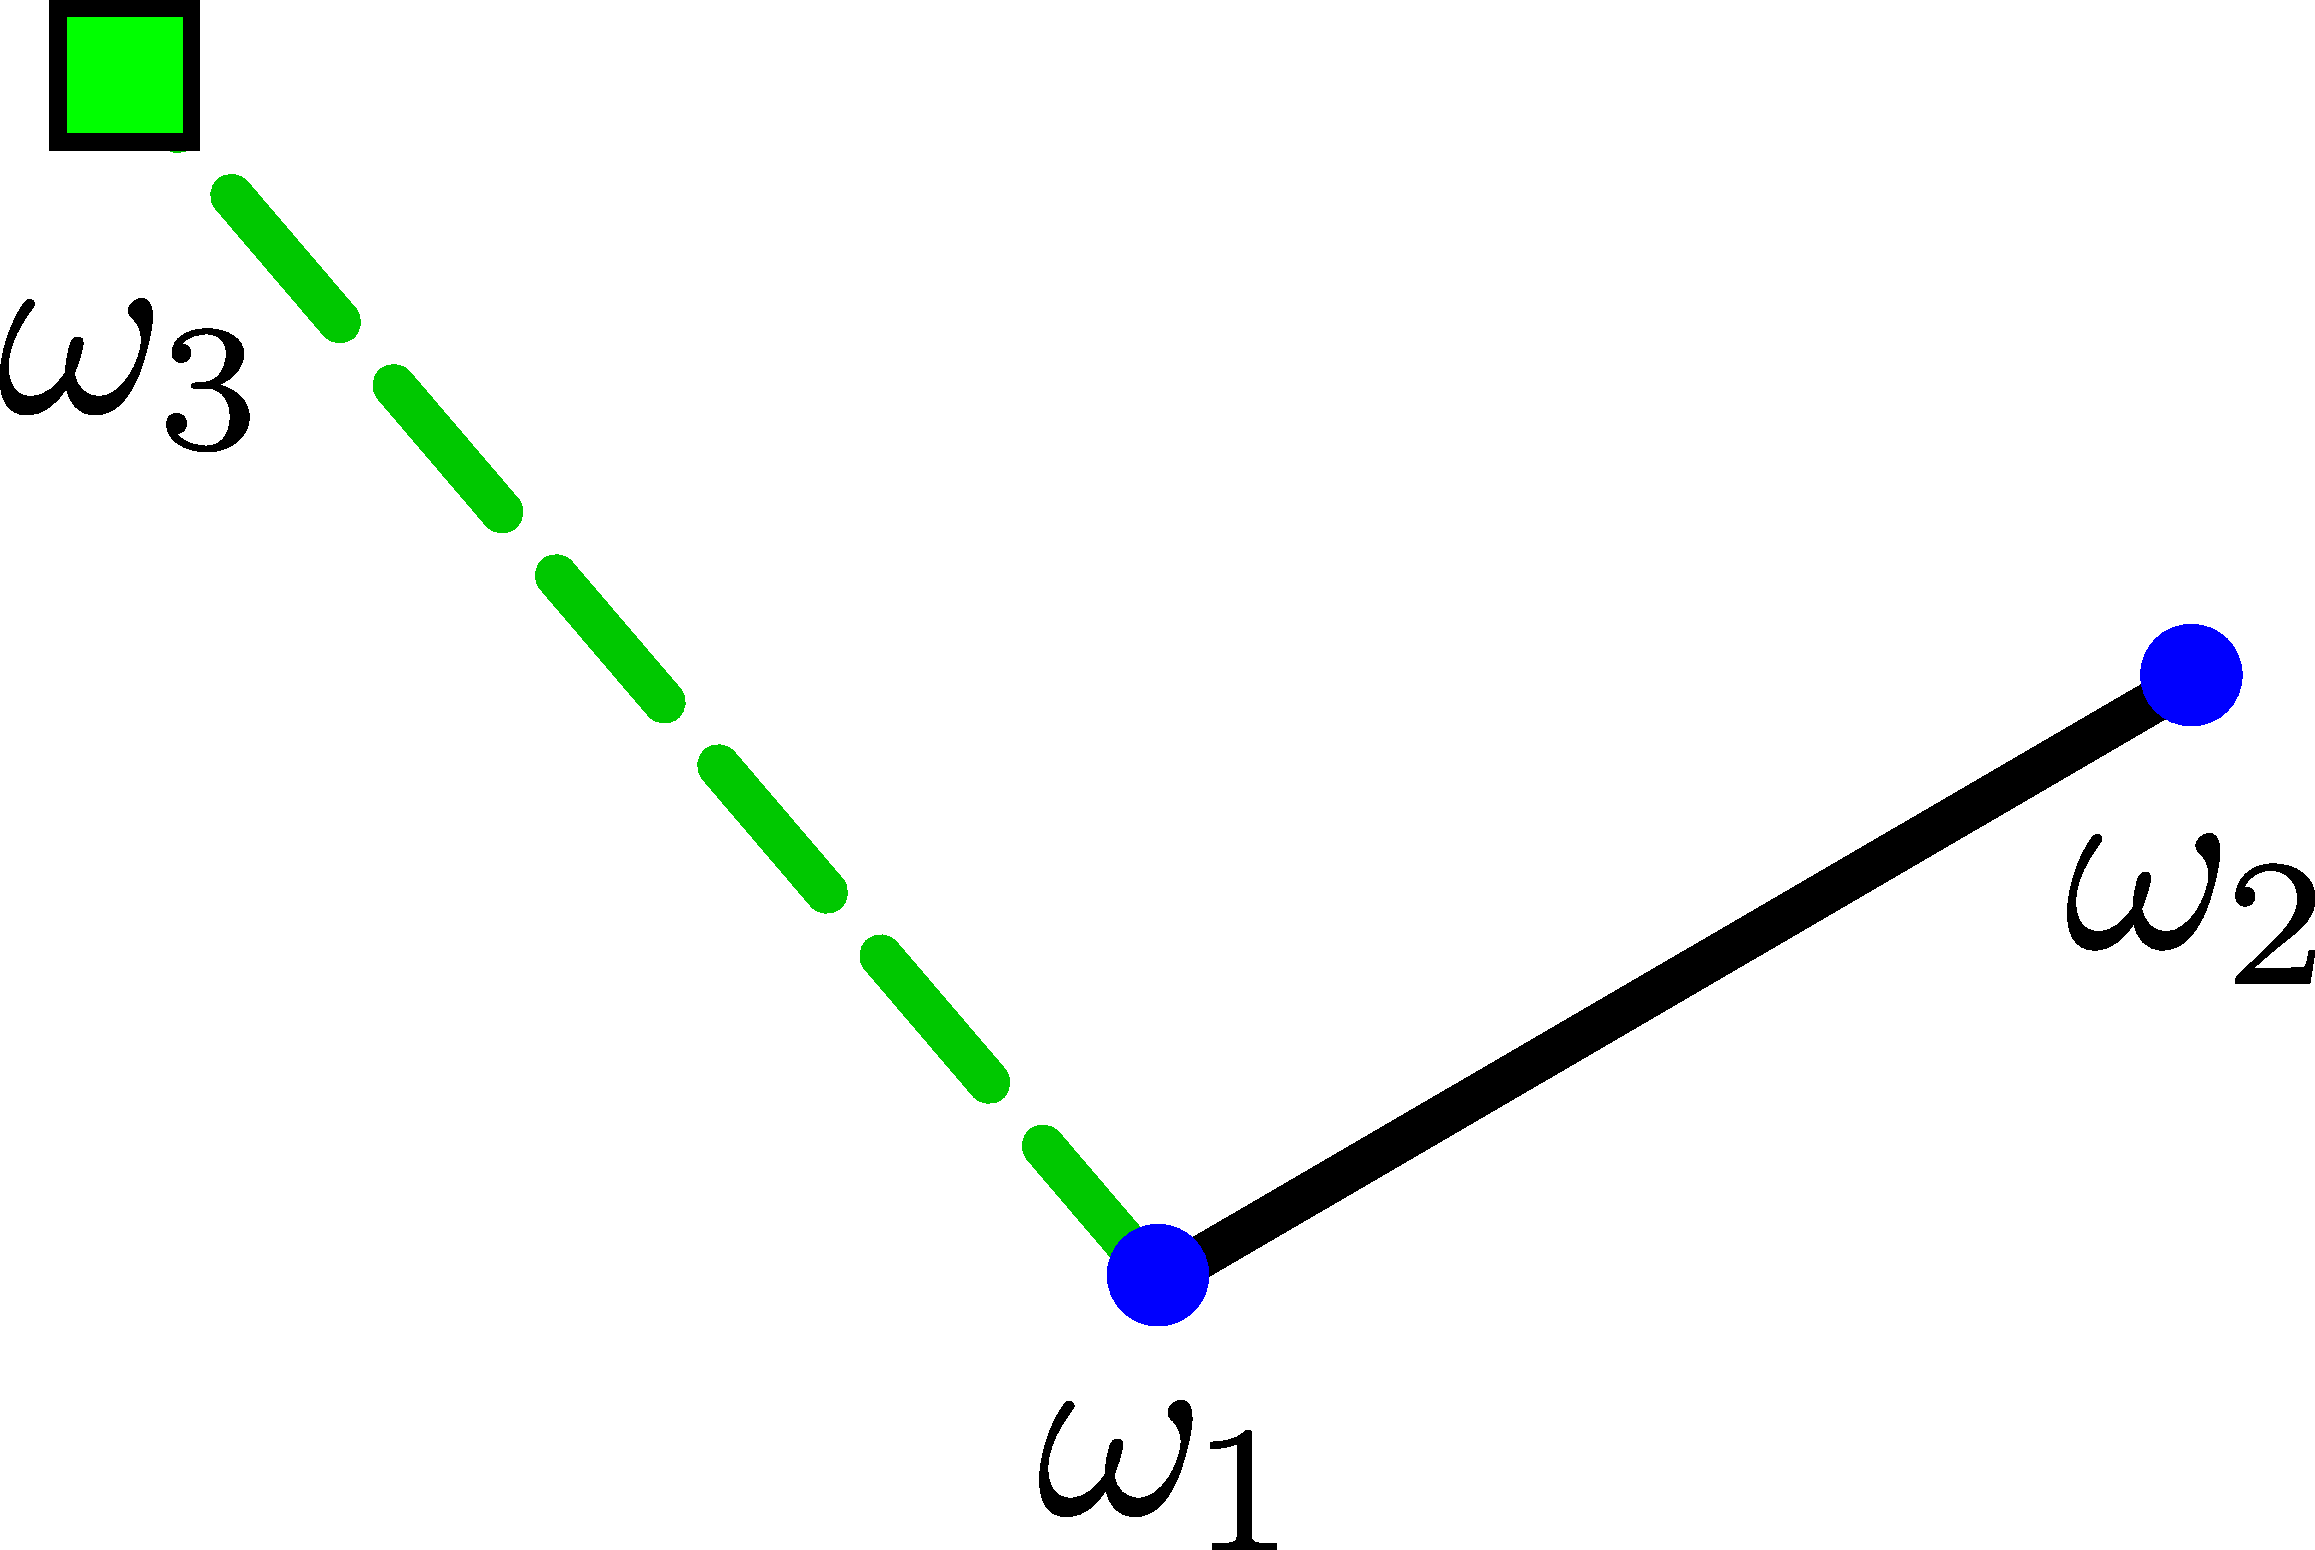
\includegraphics[scale=0.10]{fig/LEI.pdf}}
      \label{fig:injLEI}
  \label{injLEI}
  \subfloat[Internal Injection]{
      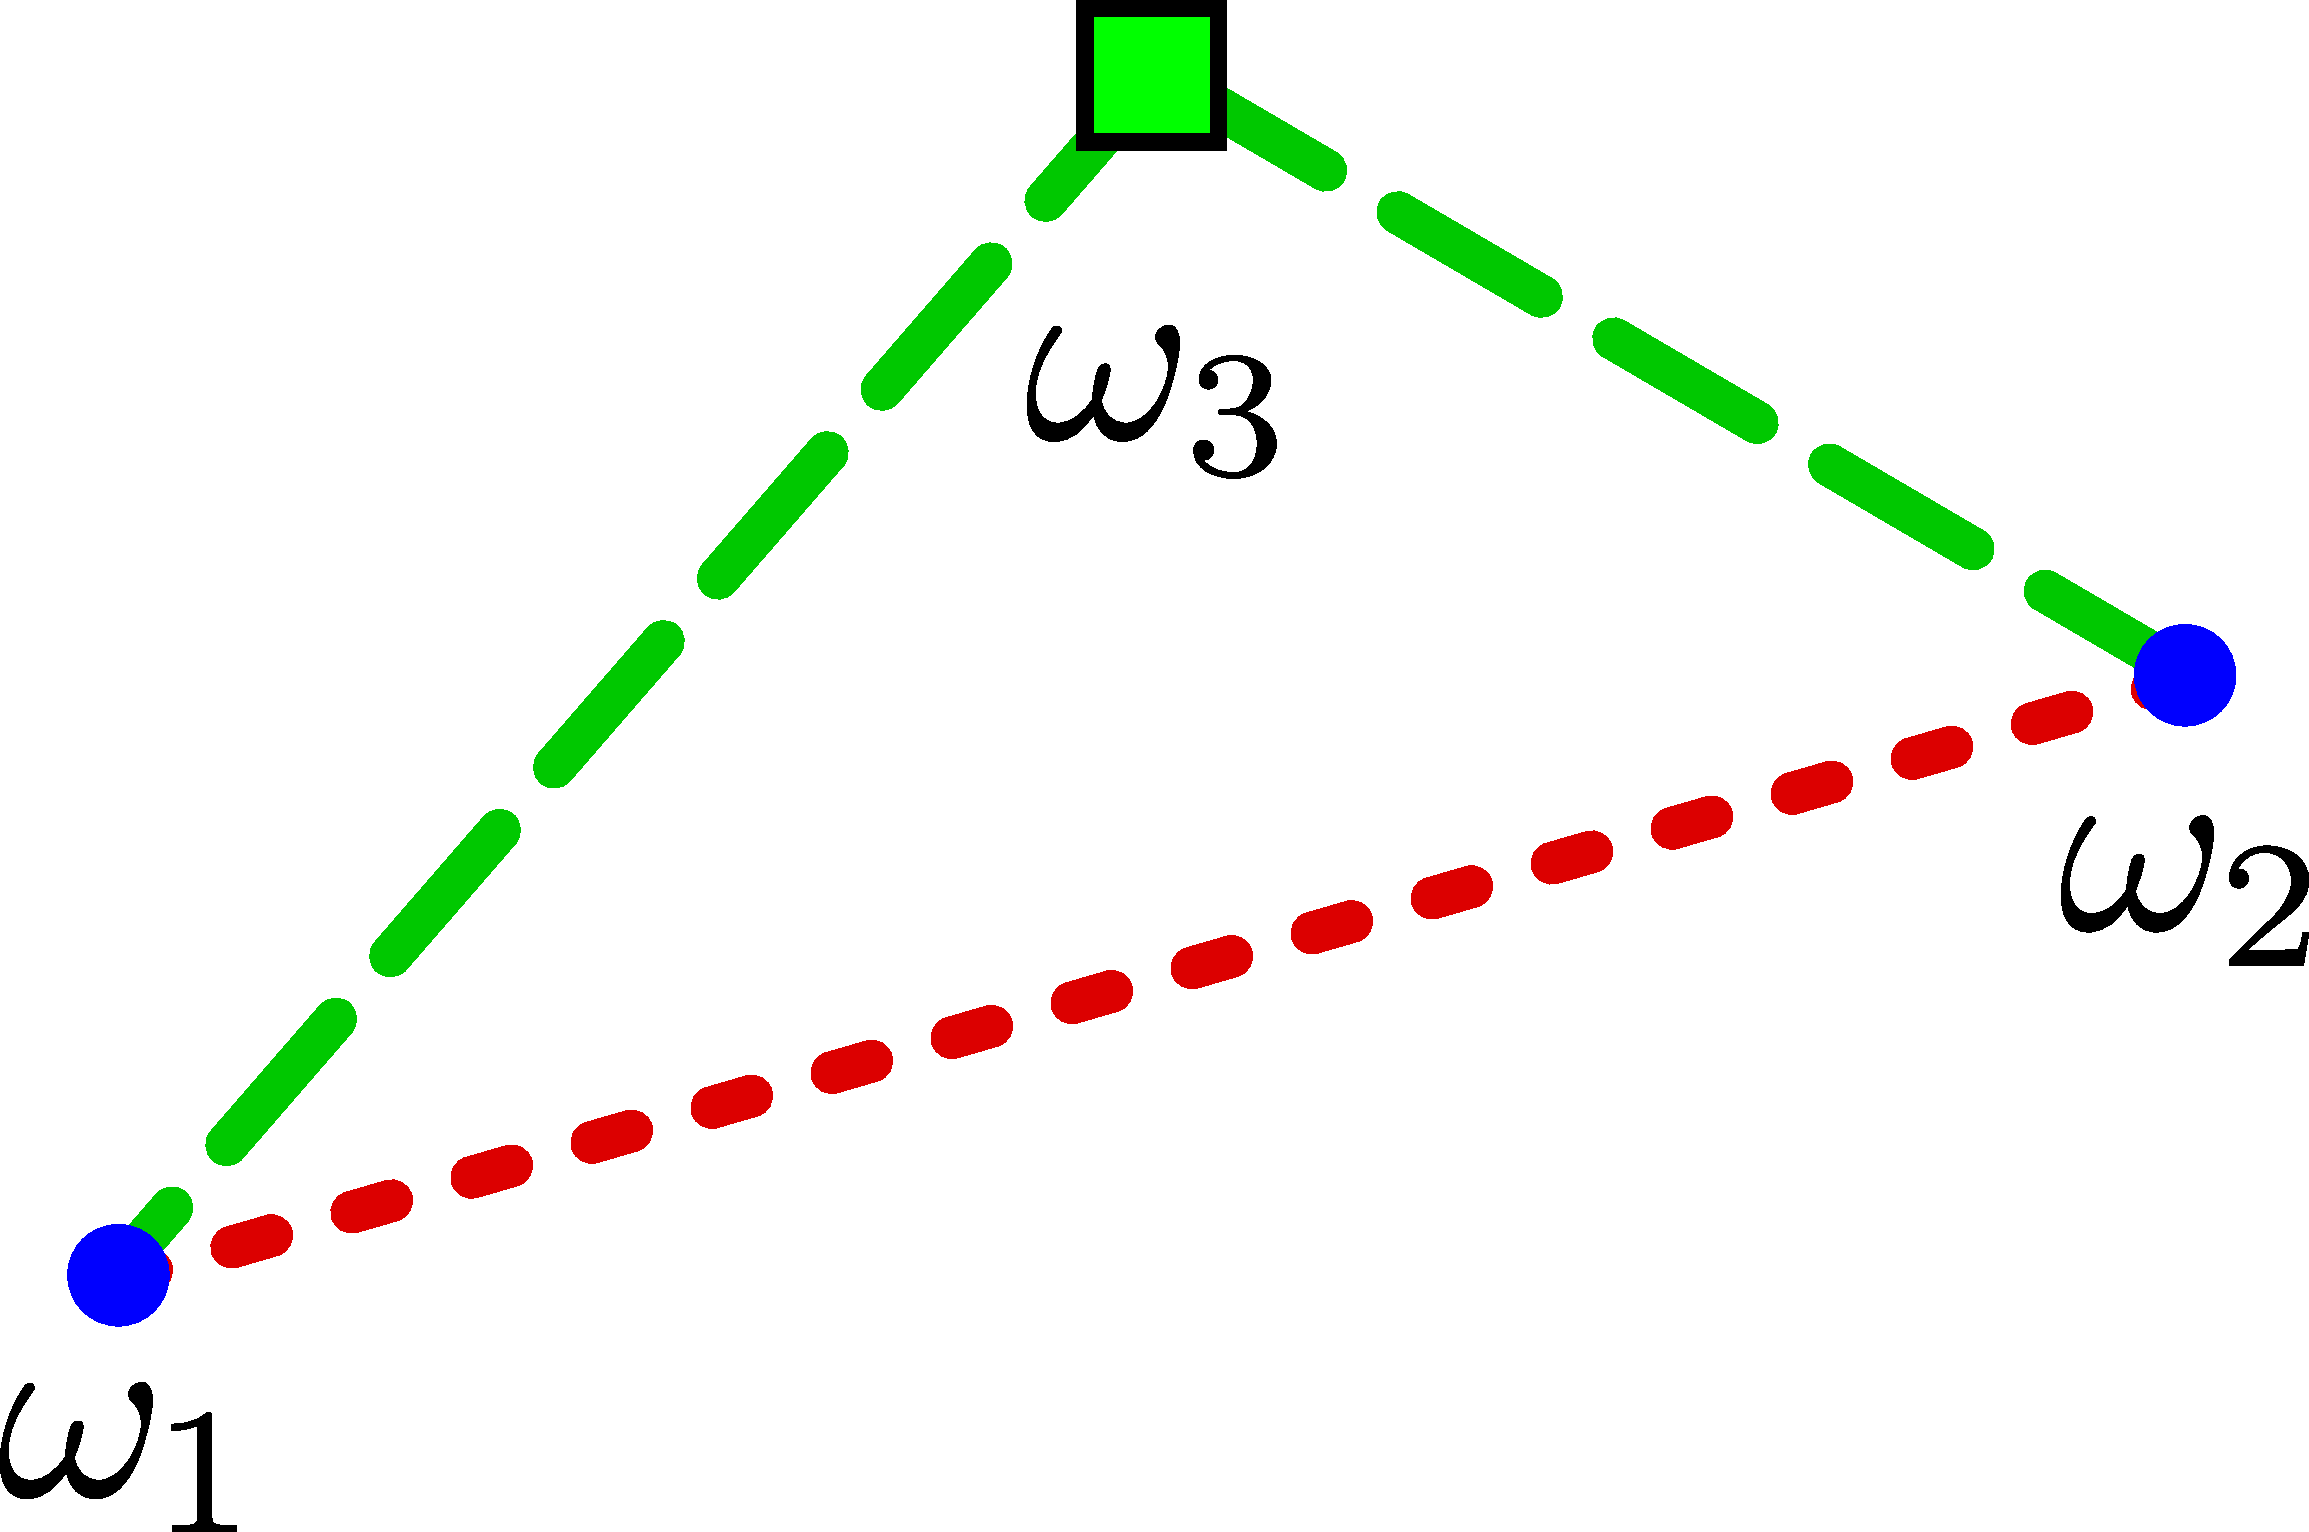
\includegraphics[scale=0.10]{fig/II.pdf}}
      \label{fig:injII}
  \label{injII}
  \subfloat[Final Injection]{
      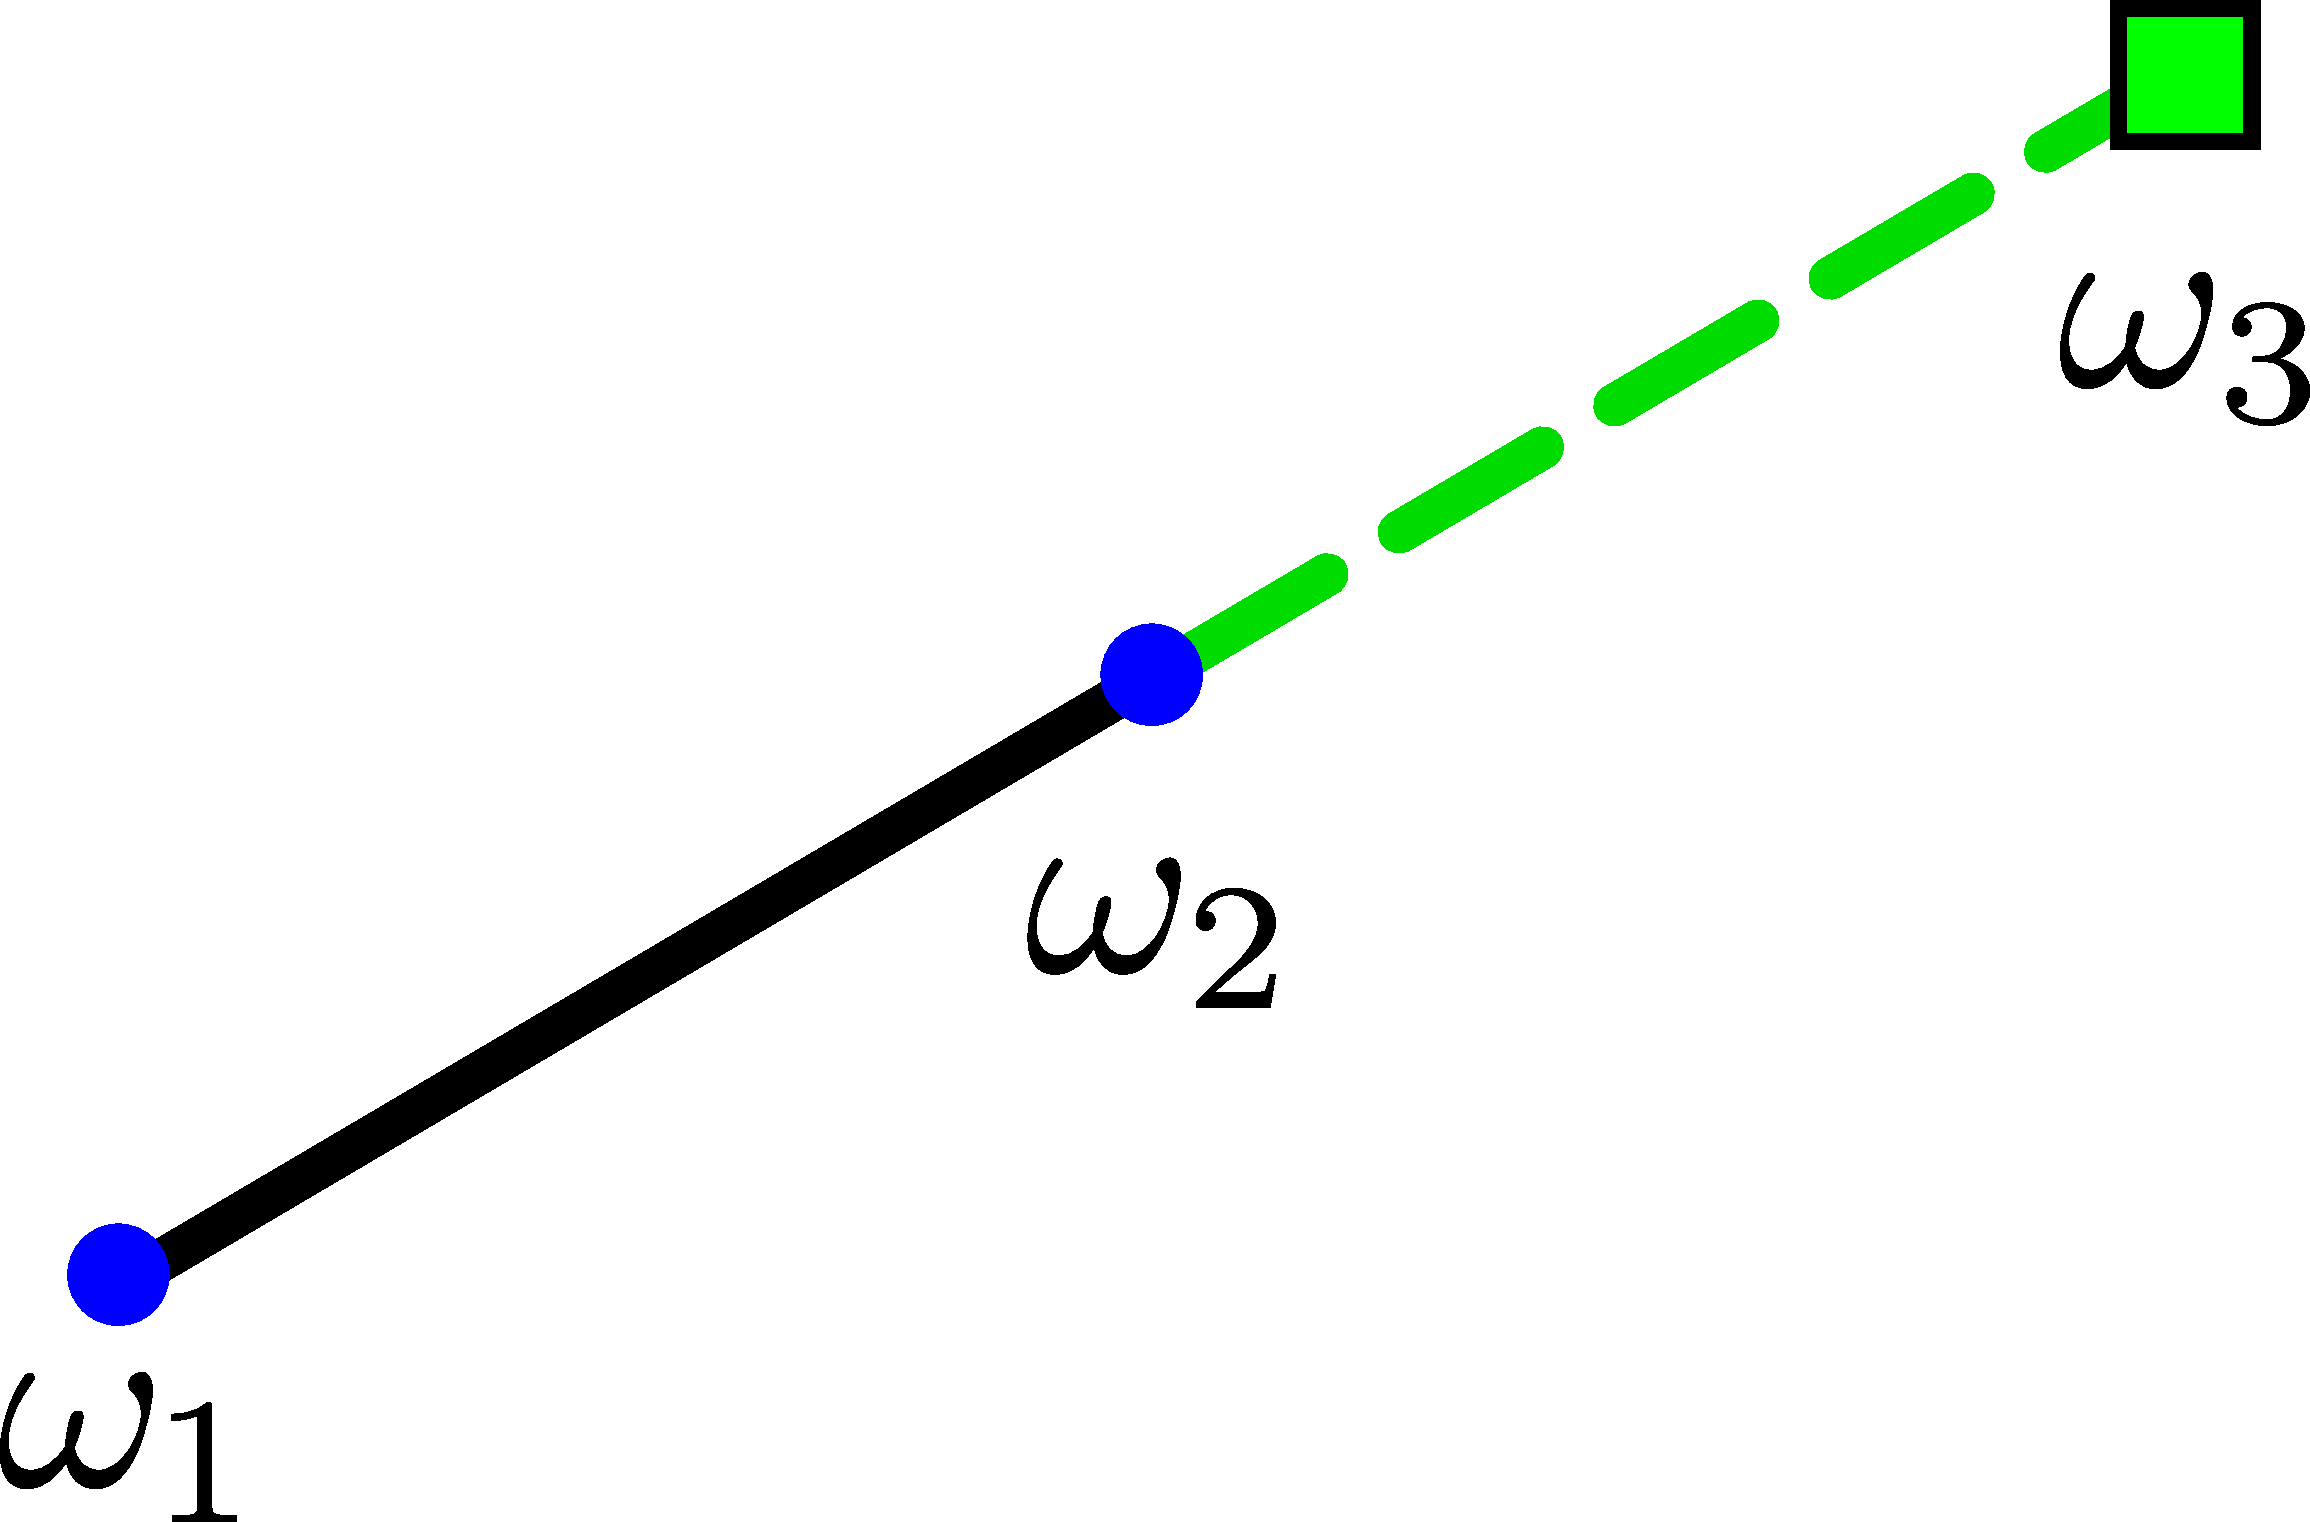
\includegraphics[scale=0.10]{fig/FEI.pdf}}
      \label{fig:injFEI}
  \label{injFEI}
%\caption{A two-speed sequence, $\omega_1, \omega_2$, shown in blue dots, receives a(n) (a) leading injection, (b) internal injection, and (c) final injection by $\omega_3$ (green square). Dashed green lines, dotted red lines, and solid black lines represent the added minimum inter-arrival times, removed minimum inter-arrival times, and unchanged minimum inter-arrival times, respectively. Green squares represent the injected speed $\omega_3$.}
\caption{Speed Injection Visualizations} A two-speed sequence, $\omega_1, \omega_2$, shown as dots, receives the (a) leading, (b) internal, and (c) final, injection of $\omega_3$ shown as a square. Dashed, dotted, and solid lines represent the added, removed, and unchanged minimum inter-arrival times, respectively.
\label{fig:injections}
\end{figure}

To compare the demand produced by two different sequences (with the same elements, but in different order), we will look at the time of the absolute deadline of the last job in the sequence under the assumptions that jobs of the sequence arrive according to their minimum interarrival time (i.e., $\widetilde{T}$) and the first job is released at time instant zero.   Let $d(S)$ be the last absolute deadline for sequence $S = (\omega_1, \ldots, \omega_n)$:
\begin{equation} \label{eq:speedSequenceTimeImplicitDeadline}
d(S) = \sum\limits_{i=1}^{n-1} \widetilde{T}(\omega_i,\omega_{i+1}) + \Tilde{d}(\omega_n).
\end{equation}

We can quantify how the $d(S)$ function changes as we inject elements of non-decreasing speed.  Let $\Delta(S, k, k+1)$ represent the amount that the $d$ function increases when injecting the $(k+1)^{th}$ smallest element ($s_{k+1}$) into $S(k)$.  That is,
\begin{equation} \label{eq:seq-delta}
\Delta(S, k, k+1) = d(S(k+1)) - d(S(k)).
\end{equation}

We can compute the above difference based on the type of injection that adding the $(k+1)^{th}$ smallest element to $S(k)$ results in:
\begin{equation} \label{eq:seq-delta-types}
\Delta(S, k, k+1) = \left\{
    \begin{array}{ll}
         \Delta_L (S, k, k+1)&{\rm if~leading},  \\
         \Delta_F (S, k, k+1)&{\rm if~final},\\
        \Delta_I (S, k, k+1)&{\rm if~internal},
    \end{array}
\right.
\end{equation}

\noindent where $\Delta_L (S, k, k+1) = \widetilde{T}(s_{k+1},\omega^{(k)}_1)$ since we are adding one segment to the front of $S(k)$ in the leading injection;   $\Delta_F (S, k, k+1) = \widetilde{T}(\omega^{(k)}_k, s_{k+1}) + \Tilde{d}(s_{k+1}) - \Tilde{d}(\omega^{(k)}_k)$ since we are adding one segment to the end of $S(k)$ and adjusting the deadline of the last job for the new speed $s_{k+1}$ for a final injection; and $\Delta_I (S, k, k+1) = \widetilde{T}(\omega^{(k)}_{j-1}, s_{k+1}) + \widetilde{T}(s_{k+1}, \omega^{(k)}_{j}) - \widetilde{T}(\omega^{(k)}_{j-1}, \omega^{(k)}_{j})$ if we inject $s_{k+1}$ into the $j^{th}$ position of $S(k)$, $j\in\mathbb{N}_2^{k}$.

We are now prepared to compare the amount of time added to the absolute deadline of the last job of the sequence, considering $k$-subsequences $S$ and $S_A$ and injecting the $(k+1)^{th}$ smallest element ($s_{k+1}$) into both of these sequences for each of the three types of injections.

\begin{property}[Leading Injection Suboptimality]\label{prop:ascending-dominates-L}
For any valid, finite sequence $S = (\omega_1, \ldots, \omega_n)$, for all $k = 1, \ldots, n-1$:
\begin{equation}\label{eqn:compare-delta-L}
    \Delta_L(S,k,k+1) \geq \Delta_F(S_A, k, k+1).
\end{equation}
\end{property}
\begin{proof}
In this property, we have a leading injection into $S(k)$.  However, observe that $\widetilde{d}(s_{k+1}) \leq \widetilde{d}({s_k})$ by Property~\ref{prop:deadline-derivative} and since $s_{k+1}$ is larger than any element of $S(k)$.  Furthermore, $\widetilde{T}(\omega^{(k)}_k, s_{k+1}) \geq \widetilde{T}(s_k, s_{k+1})$ since, by Property~\ref{prop:neg-deriv-min-interarrival}, $\widetilde{T}$ is a decreasing function in its parameters and $s_k$ is at least as large as any item in $S(k)$.  Also, by Property~\ref{T-reversal}, $\widetilde{T}(\omega^{(k)}_k, s_{k+1})$ equals $\widetilde{T}(s_{k+1}, \omega^{(k)}_k)$.  By the above observations, we get:
\begin{equation}\label{eq:FEIdominatesLEI}
\begin{array}{ll}                  
    & \widetilde{T}(s_{k+1}, \omega^{(k)}_k) +\Tilde{d}(s_k) \geq \widetilde{T}(s_k, s_{k+1})+\Tilde{d}(s_{k+1})\nonumber\\
    \Leftrightarrow & \widetilde{T}(s_{k+1}, \omega^{(k)}_k) \geq \widetilde{T}(s_k, s_{k+1})+\Tilde{d}(s_{k+1})- \Tilde{d}(s_k)\nonumber
\end{array}
\end{equation}

The LHS and RHS of the last inequality matches  Equation~\ref{eqn:compare-delta-L} and the lemma is proved.
\end{proof}



\begin{property}[Internal Injection Suboptimality]\label{prop:ascending-dominates-I}
For any valid, finite sequence $S = (\omega_1, \ldots, \omega_n)$, for all $k = 1, \ldots, n-1$:
\begin{equation}\label{eqn:compare-delta-I}
    \Delta_I(S,k,k+1) \geq \Delta_F(S_A, k, k+1).
\end{equation}
\end{property}
\begin{proof}
Observe that by Properties~\ref{T-reversal} and~\ref{prop:deadline-derivative}, $\widetilde{T}(f,\omega + \epsilon) \geq \tilde{d}(\omega + \epsilon)$ for all $f, \omega$ and $\epsilon > 0$.  Also, $\widetilde{T}(s_k +\epsilon, \omega) = \widetilde{T}(\omega, s_k+\epsilon)$ for all $\omega$ and $\epsilon >0$ by Property~\ref{T-reversal}. These properties imply that:
\begin{equation}\label{eqn:change-sk}
\begin{array}{ll}
     & 
     \begin{array}{ll}
        \lefteqn{\widetilde{T}(s_{k-1},s_k) + \widetilde{T}(s_k, s_k) + \tilde{d}(s_k)}& \\
            &= \widetilde{T}(s_{k-1},s_k) + \widetilde{T}(s_k,s_k) + \tilde{d}(s_k)
      \end{array}\\
     \Rightarrow & 
     \begin{array}{ll}
        \lefteqn{\widetilde{T}(s_{k-1},s_k +\epsilon) + \widetilde{T}(s_k+\epsilon, s_k) + \tilde{d}(s_k)}& \\
        &\geq \widetilde{T}(s_{k-1},s_k) + \widetilde{T}(s_k, s_k + \epsilon) + \tilde{d}(s_k+\epsilon) 
    \end{array}\\
\end{array}
\end{equation}

\noindent Setting $\epsilon = s_{k+1} - s_k$ and substituting into the above inequality of Equation~\ref{eqn:change-sk}, we get the following:
\begin{equation}\label{eqn:change-sk2}
\begin{array}{ll}
     &\begin{array}{ll}
        \lefteqn{\widetilde{T}(s_{k-1},s_{k+1}) + \widetilde{T}(s_{k+1}, s_k) + \tilde{d}(s_k)}& \\
        &\geq \widetilde{T}(s_{k-1},s_k) + \widetilde{T}(s_k, s_{k+1}) + \tilde{d}(s_{k+1}) 
    \end{array}\\
    \Rightarrow&
    \begin{array}{ll}
        \lefteqn{\widetilde{T}(s_{k-1},s_{k+1}) + \widetilde{T}(s_{k+1}, s_k) - \widetilde{T}(s_{k-1},s_k)}& \\
        &\geq \widetilde{T}(s_k, s_{k+1}) + \tilde{d}(s_{k+1}) - \tilde{d}(s_k)
    \end{array}\\
    \Rightarrow&
    \begin{array}{ll}
        \lefteqn{\widetilde{T}(\omega^{(k)}_{j-1}, s_{k+1}) + \widetilde{T}(s_{k+1},\omega^{(k)}_{j}) - \widetilde{T}(\omega^{(k)}_{j-1},\omega^{(k)}_{j})} &\\
        &\geq \widetilde{T}(s_k, s_{k+1}) + \tilde{d}(s_{k+1}) - \tilde{d}(s_k) \\
    \end{array}\\
\end{array}
\end{equation}
% \sandeep{Why are we only changing $s_k$ to $\omega^{(k)}_{j}$ on the left hand side of the last inequality and not the right side?}
\noindent The last inequality (which implies Equation~\ref{eqn:compare-delta-I} of the property) above follows from observing that according to Property~\ref{prop:neg-deriv-min-interarrival}, the following is true for all $\omega$ and $\omega'$:
\begin{equation}
\begin{array}{ll}
        &\frac{\partial \widetilde{T}(\omega,s_{k+1})}{\partial \omega}
            \leq \frac{\partial \widetilde{T}(\omega,\omega')}{\partial \omega} \nonumber\\
        \Leftrightarrow&
        \frac{\partial \widetilde{T}(\omega,s_{k+1})}{\partial \omega} + \frac{\partial \widetilde{T}(s_{k+1},\omega')}{\partial \omega} - \frac{\partial \widetilde{T}(\omega,\omega')}{\partial \omega} \leq 0 \nonumber  
\end{array}
\end{equation}
\noindent  Thus, the LHS of the second inequality of Equation~\ref{eqn:change-sk2} will not decrease if we substitute $\omega^{(k)}_{j-1}$ for $s_{k-1}$ in the LHS.  For symmetric reasons, we can also substitute $\omega^{(k)}_{j}$ for $s_k$.
\end{proof}

%\fishern{Making a pass from this point -- 1:10am 6/1}

In this next property, we show that any sequence may decrease the time of its last deadline by moving the highest speed job to the end (if it is valid).  The proof of this property is in the appendix.

\begin{property}[Highest-Speed Relative-Deadline Dominance]\label{prop:high-speed-transfer}
For any valid, finite sequence $S = (\omega_1, \ldots, \omega_n)$, if $\omega_\ell$ ($\ell \in \mathbb{N}_1^n-1$) is the highest speed $s_n$ and not the last speed of sequence $S$ and $s_n \leq \Omega_1(\omega_n,\alpha_{\max})$ then new sequence $S'$ with the highest element moved to the last element (i.e., $S' = (\omega_1, \ldots, \omega_{\ell-1}, \omega_{\ell+1}, \ldots, \omega_n, s_n)$) is valid and has the following property: 
\begin{equation}\label{eqn:high-speed-transfer}
    d(S) \geq d(S').
\end{equation}
\end{property}

We are now ready to state the main lemma of this subsection.  That is, for any dominant speed sequence, we can find another dominant speed sequence with equivalent demand that is in ascending order.

\begin{lemma}[Dominant Non-Decreasing Speed Sequences]\label{lemma:non-decreasing}
Given a valid, dominant speed sequence $S = (\omega_1, \omega_2, \ldots, \omega_n)$ over interval $[t_a, t_b]$, the sequence $S_A$ is valid and has equivalent demand.
\end{lemma}
\begin{proof}
The proof is by induction on $k$.  For each $k \in \mathbb{N}_1^n$, we show that for any $k$-subsequence $S'(k)$ containing the same elements of $S(k)$ such that $d(S(k)) \geq d(S'(k))$, the following is true:
\begin{equation}\label{eqn:non-decr-IH}
    d(S(k)) \geq d(S'(k)) \geq d(S_A(k)).
\end{equation}
\noindent This implies the lemma, since if the deadline of the last job of $S$ is before $t_b$, then the last job of $S_A$ must also be before $t_b$; therefore, the demand over the interval does not decrease when reordering $S$ to non-decreasing order.
 
\noindent \emph{Base Case}: Consider when $k=1$, clearly $S(1)=S_A(1) = (s_1)$.  Thus, Equation~\ref{eqn:non-decr-IH} is vacuously true.

\noindent \emph{Induction Hypothesis}:  Assume that Equation~\ref{eqn:non-decr-IH} holds up to some $k < n$ for all $S'(k)$ containing the same elements of $S(k)$ such that $d(S(k)) \geq d(S'(k))$.

\noindent \emph{Inductive Step}:  We need to show that Equation~\ref{eqn:non-decr-IH} is true for $k+1$.  Let $S'(k)$ be any $k$-subsequence.  We now consider injecting $s_{k+1}$ into $S'(k)$ and $S_A(k)$.  (Note that $S_A$ and $S'_A$ are identical subsequences).  There are three cases depending on the type of injection into $S'(k)$.
\begin{case}[Leading Injection]
  By Property~\ref{prop:ascending-dominates-L}, $\Delta_L(S',k,k+1) \geq \Delta_F(S_A,k,k+1)$.  Therefore, by the Induction Hypothesis, $d(S'(k+1)) = d(S'(k))+ \Delta_L(S',k,k+1)\geq d(S_A(k)) + \Delta_F(S_A,k, k+1) = d(S_A(k+1))$.  
\end{case}
\begin{case}[Internal Injection]
  By Property~\ref{prop:ascending-dominates-I}, $\Delta_I(S',k,k+1) \geq \Delta_F(S_A,k,k+1)$.  Therefore, by the Induction Hypothesis, $d(S'(k+1)) = d(S'(k))+ \Delta_I(S',k,k+1)\geq d(S_A(k)) + \Delta_F(S_A,k, k+1) = d(S_A(k+1))$.  
\end{case}
\begin{case}[Final Injection]
  By Property~\ref{prop:high-speed-transfer}, there exist a valid sequence $S''(k)$ obtained from $S'(k)$ by moving the highest term ($s_k$) to the end of $S''(k)$ where $d(S'(k))\geq d(S''(k))$.   (If $S'(k)$ already had $s_k$ as its last term, then $S''(k) = S'(k)$).  By Induction Hypothesis, $d(S''(k)) \geq d(S_A(k))$.
  Since the last term on $S'(k)$ and $S_A$ is identical, $\Delta_F(S',k, k+1)$ equals $\Delta_F(S_A,k,k+1)$.  Observe that $\Delta_F(S',k, k+1) \geq \Delta_F(S'', k, k+1)$ since the last element in $S''$ is $s_k$ and Property~\ref{prop:deadline-derivative} implies $S''$ will have less time added to its deadline.  Therefore, we have $d(S'(k))+\Delta_F(S',k,k+1) \geq d(S''(k)) + \Delta_F(S'',k,k+1) \geq d(S_A(k)) + \Delta_F(S_A,k,k+1)$. Hence, $d(S'(k+1))\geq d(S_A(k+1))$.
\end{case}
In all the cases, we show that for all $S'$ such that $d(S(k+1)) \geq d(S'(k)) \Rightarrow d(S'(k)) \geq d(S_A(k))$ which proves the lemma.
\end{proof}






%%%%%%%%%%%%%%%%BEGIN COMMENT%%%%%%%%%%%%%%%%%%%%%
\begin{comment}
\paragraph{Speed Sets and Sequences}

The following model is established to describe speed sequences:
\begin{enumerate}
\item $\mathcal{S}$ is a \textit{Speed Set}, an ordered, finite set of speeds where $\mathcal{S}=(\omega_1, \omega_2, \omega_3,...,\omega_n) \quad | \quad \omega_i \leq \omega_j \quad \forall i<j$. 
\item $\mathcal{S}(k)$ is a \textit{Speed Subset}, an unordered, finite subset of $\mathcal{S}$ containing the $k$ lowest speeds in $\mathcal{S}$. More formally, $\mathcal{S}(k) \subseteq S \quad | \quad S(k) = \{s_1, s_2, ... , s_k\} : k \leq n$.
\item $Q(\mathcal{S}(k))$ is a \textit{Speed Sequence}, an ordered permutation of $\mathcal{S}$ where $Q(\mathcal{S}(k))=(q_1, q_2, q_3, ... , q_k)$ %\quad | \quad \forall i \in \mathbb{Z} \quad | \quad 0 < i < n$
\item $Q_{A}(\mathcal{S}(k))$ is an \textit{Ascending Speed Sequence}, an ordered permutation of $\mathcal{S}$ where $Q_{A}(\mathcal{S}(k))=(q_1, q_2, q_3, ... , q_k) \: | \: q_i = s_i \: \forall i \in \mathbb{N}_1 : 1 \leq i \leq k$
\item $\mathcal{Q}(S)$ is a \textit{Sequence Space}, a set of all ordered permutations of $\mathcal{S}$.
\item $\mathcal{Q}_{feasible}(\mathcal{S}(k))$ is a \textit{Feasible Sequence Space}, the set of all $Q(\mathcal{S}(k))$ where \\ $q_{i+1} \leq \sqrt{q_i^{2} + 2\alpha_{\max}} \quad \forall i \in \mathbb{Z} \: | \: 1 \leq i \leq n-1 \:$.
\end{enumerate}

\subsubsection{Speed Injections}
equations describe speed injections, sequence transformations for manipulating speed sequences by adding a speed $\omega_{k+1}$ to a $Q(\mathcal{S}(k))$.
\subparagraph{Leading External Injection}
A Leading External Injection is a transformation defined as:
\begin{equation}
\textbf{T}_{LEI}(Q(\mathcal{S}(k)),\omega_{k+1}) = Q'(\mathcal{S}(k+1)) \: | \: q'_1 = \omega_{k+1}
\end{equation}
%where $Q'(\mathcal{S}(k+1))$ has $\omega_{k+1}$ as the first speed.
which causes an increase in sequence time:
\begin{equation}\label{eq:injLeading}
\Delta t_{LEI}(Q(\mathcal{S}(k)),\omega_{k+1}) = m(\omega_{k+1},q_1)
\end{equation}
Note that Equation \ref{eq:injLeading} is minimized when $q_1 = \omega_k$.
\subparagraph{Internal Injection}
An Internal Injection is a transformation defined as:
\begin{equation}
\textbf{T}_{II}(Q(\mathcal{S}(k)),q_x,\omega_{k+1}) = Q'(\mathcal{S}(k+1)) \: | \: q'_{x+1} = \omega_{k+1}
\end{equation}
where $1 \leq x < k-1$ with the increase in sequence time:
\begin{alignat}{3} \label{eq:injInternal}
&\Delta t_{II}(Q(\mathcal{S}(k)),q_x,\omega_{k+1}) =& \nonumber \\
&m(q_x,\omega_{k+1}) + m(\omega_{k+1}, q_{x+1}) - m(q_x,q_{x+1})&
\end{alignat}
Note Equation \ref{eq:injInternal} is minimized when $q_x = \omega_k, q_{x+1} = \omega_{k-1}$.
\subparagraph{Final External Injection}
A Final External Injection is a transformation which inserts a speed into a sequence defined as:
\begin{equation}
\textbf{T}_{FEI}(Q(\mathcal{S}(k)),\omega_{k+1}) = Q'(\mathcal{S}(k+1)) \: | \: q'_k = \omega_{k+1}
\end{equation}
For final external injections, the increase in time is defined as:
\begin{alignat}{3}\label{eq:injFinal}
&\Delta t_{FEI}(Q(\mathcal{S}(k)),\omega_{k+1}) = \nonumber \\ &m(q_k,\omega_{k+1}) + E(\omega_{k+1}) - E(q_k)
\end{alignat}
Note that Final External Injection of $\omega_{k+1}$ into $Q_{A}(S(k))$ will maintain the ascending property of the sequence permutation.


\begin{lemma}[Dominant Non-Decreasing Speed Sequences]\label{lemma:non-decreasing}
Given a speed set, $\mathcal{S}$, of size $n$, the ascending speed sequence, $Q_{A}(S(k))$ in which speeds are traversed in increasing order gives the fastest speed sequence time. Formally, $\Delta_t(Q_{A}(S(k))) \leq \Delta_t(Q(S(k)) \: \forall k \in \mathbb{N}_1 : 1 \leq k \leq n, \; S(k), \; Q(S(k)) \in \mathcal{Q}_{feasible}(S(k))$.
\end{lemma}
\begin{proof}
\subparagraph{Base Case - $\Delta_t(Q(\mathcal{S}(1))) \leq \Delta_t(Q_{A}(\mathcal{S}(1)))$}
By Equations \ref{eqn:deadline-derivative} and \ref{eq:speedSequenceTimeImplicitDeadline}, an initial $Q_{A}(\mathcal{S}(1))$ is equivalent to any $Q(\mathcal{S}(1)) \in \mathcal{Q}_{feasible}(\mathcal{S}(1))$.
Since $\mathcal{S}(1)$ contains only one speed and has only one permutation, $Q(\mathcal{S}(1))$ is an ascending sequence such that $Q(\mathcal{S}(1)) = Q_{A}(\mathcal{S}(1))$.
Therefore, $\Delta_t(Q(\mathcal{S}(1))) \leq \Delta_t(Q_{A}(\mathcal{S}(1)))$, is true.
\subparagraph{Inductive Step - $Q(\mathcal{S}(k)) \leq Q_{A}(\mathcal{S}(k))$}
Given a speed set, $S$, and sequence permutation $Q(\mathcal{S}(k))$, the sequence permutation $Q(\mathcal{S}(k))$ can be constructed via a series of transformations: Leading External, Internal, or Final External speed injections. For example, $Q(\mathcal{S}(1))$ may be transformed into $Q(\mathcal{S}(2))$ via Equations \ref{eq:injLeading} or \ref{eq:injFinal}: $\textbf{T}_{LEI}(Q(\mathcal{S}(1)),\omega_{2})$ or $\textbf{T}_{FEI}(Q(\mathcal{S}(k)),\omega_{k+1})$. However, $Q(\mathcal{S}(2))$ contains too few elements yet for Equation \ref{eq:injInternal}, $\textbf{T}_{II}(Q(\mathcal{S}(1)),q_x,\omega_{2})$.

The following cases compare and establish dominant sequence transformations and sequences:
\begin{case}[Minimum Leading External Injection]
Ascending Final External Injection into $Q_{A}(\mathcal{S}(k))$ adds less time than ascending Leading External Injection to any $Q(\mathcal{S}(k))$.
\end{case}
Suppose $Q(\mathcal{S}(k))$ is ordered such that $q_1 = \omega_k$ in Equation \ref{eq:injLeading}. $\Delta t_{FEI}(Q_{A}(\mathcal{S}(k)),\omega_{k+1})$ will be minimized for all possible $q_1$ and compares as follows:
\begin{alignat}{4} \label{eq:FEIdominatesLEI}
&& E(\omega_k) & \geq E(\omega_{k+1}) &\quad& \nonumber \\
\Leftrightarrow && \widetilde{T}(\omega_{k+1},q_1) + E(\omega_k) & \geq \widetilde{T}(\omega_k,\omega_{k+1}) + E(\omega_{k+1}) &\quad& \nonumber \\
\Leftrightarrow && \widetilde{T}(\omega_{k+1},q_1) & \geq \widetilde{T}(\omega_k,\omega_{k+1}) + E(\omega_{k+1}) &\quad& \nonumber \\
\Leftrightarrow && \Delta t_{LEI}(Q(\mathcal{S}(k)),\omega_{k+1}) & \geq \Delta t_{FEI}(Q_{A}(\mathcal{S}(k)),\omega_{k+1}) && %\\
%&& & \qquad \qquad \qquad \text{By Eq. \ref{eq:injFinal}} \nonumber
\end{alignat}

\begin{case}[Minimum Internal Injection]\label{case:optimalInternalInjection}
Ascending final external injection adds less time to $Q_{A}(\mathcal{S}(k))$ than ascending internal external injection to any $Q(\mathcal{S}(k))$.
\end{case}
Suppose $Q(\mathcal{S}(k))$ is ordered such that $q_x = \omega_{k-1}, q_{x+1} = \omega_{k+1}$ in Equation \ref{eq:injInternal}. $\Delta t_{II}(Q(\mathcal{S}(k)),q_x,\omega_{k+1})$ will be minimized for all possible $q_x, q_{x+1}$ and compares as follows.
Let $a = \omega_{k-1}$, $b = c = \omega_k$, and $\delta = \omega_{k+1}-\omega_k$ and compare a partial increase $\delta$ in $b$ versus $c$ by the following equations:
\begin{alignat}{4}\label{eq:FEIdominatesII}
&& \widetilde{T}(a,b) + \widetilde{T}(b,c) + E(c) & = \widetilde{T}(a,b) + \widetilde{T}(b,c) + E(c) & \nonumber \\
\Leftrightarrow && \widetilde{T}(\omega_{k-1},\omega_k) + \widetilde{T}(\omega_k,\omega_k) + E(\omega_k) & = \widetilde{T}(\omega_{k-1},\omega_k) + \widetilde{T}(\omega_k,\omega_k) + E(\omega_k) & \nonumber \\
\Leftrightarrow && \widetilde{T}(\omega_{k-1},\omega_k+\delta) + \widetilde{T}(\omega_k+\delta,\omega_k) + E(\omega_k) & \geq \widetilde{T}(\omega_{k-1},\omega_k) + \widetilde{T}(\omega_k,\omega_k+\delta) + E(\omega_k+\delta) & \nonumber \\
\Leftrightarrow && \widetilde{T}(\omega_{k-1},\omega_{k+1}) + \widetilde{T}(\omega_{k+1},\omega_k) + E(\omega_k)& \geq  \widetilde{T}(\omega_{k-1},\omega_k) + \widetilde{T}(\omega_k,\omega_{k+1}) + E(\omega_{k+1}) & \nonumber \\
\Leftrightarrow && \widetilde{T}(q_x,\omega_{k+1}) + \widetilde{T}(\omega_{k+1},q_{x+1}) - \widetilde{T}(\omega_{k-1},\omega_k) & \geq  \widetilde{T}(\omega_k,\omega_{k+1}) + E(\omega_{k+1}) - E(\omega_k) & \nonumber \\
\Leftrightarrow && \Delta t_{II}(Q(\mathcal{S}(k)),q_x,\omega_{k+1}) & \geq \Delta t_{FEI}(Q_{A}(\mathcal{S}(k)),\omega_{k+1}) &\quad& \text{By Eq. \ref{eq:injFinal}}
\end{alignat}

\begin{case}[Highest Speed Transfers for $q_k \neq \omega_k$] Highest Speed Transfers are time-reducing transformations which apply to sequences where $q_k \in Q(\mathcal{S}(k)) \neq \omega_k$. If $\textbf{T}_{HST}(Q(\mathcal{S}(k))$ is infeasible, $\textbf{T}_{FEI}(Q(\mathcal{S}(k),\omega_{k+1})$ is also infeasible.
\end{case}
\begin{proof}
By Equation \ref{eq:HST}, Highest Speed Transfers transform $Q(\mathcal{S}(k))$ into $Q'(\mathcal{S}(k)) \:|\: q'_k = \omega_k$ and all transfers are time-reducing by Lemma \ref{lem:HST}. However, this transformation is feasible only when the highest speed $\omega_k$ is reachable from the final speed $q_k$ such that $\omega_k \leq \sqrt{q_k^2 + 2\alpha_{\max}}$. If $\textbf{T}_{HST}(Q(\mathcal{S}(k))$ is infeasible, $\omega_k > \sqrt{q_k^2 + 2\alpha_{\max}} \implies \omega_{k+1} > \sqrt{q_k^2 + 2\alpha_{\max}}$ since $\omega_k \leq \omega_{k+1}$ by the definition of $\mathcal{S}(k)$.
\end{proof}
\begin{case}[Equivalent Final External Injection] Ascending final external injection into $Q_{A}(\mathcal{S}(k))$ adds time equal to ascending internal external injection to any $Q(\mathcal{S}(k))$.
\end{case}
\begin{proof}
Suppose the final jobs of $Q(\mathcal{S}(k))$ and $Q_{A}(\mathcal{S}(k))$ equal such that $q_k \in Q(\mathcal{S}(k)) = q_k \in Q_{A}(\mathcal{S}(k))$, let $a = \omega_k, b = \omega_{k+1}$ and compare as follows:
\begin{alignat}{4}\label{eq:FEIequalsFEI}
&& \widetilde{T}(a,b) + E(b) - E(a) & = \widetilde{T}(a,b) + E(b) - E(a)  & \nonumber \\
\Leftrightarrow && \widetilde{T}(\omega_k,\omega_{k+1}) + E(\omega_{k+1}) & = \widetilde{T}(\omega_k,\omega_{k+1}) + E(\omega_{k+1}) \nonumber \\
&& - E(\omega_k) & \phantom{{}={}} - E(\omega_k) \nonumber \\
\Leftrightarrow && \Delta t_{FEI}(Q(\mathcal{S}(k)),\omega_{k+1}) & = \Delta t_{FEI}(Q_{A}(\mathcal{S}(k)),\omega_{k+1}) &
\end{alignat}
\end{proof}
By Equation \ref{eq:speedSequenceTimeImplicitDeadline}, an initial $Q_{A}(\mathcal{S}(1))$ is equivalent to any $Q(\mathcal{S}(1)) \in \mathcal{Q}_{feasible}(\mathcal{S}(1))$. Furthermore, $Q_{A}(\mathcal{S}(2))$ dominates any $Q(\mathcal{S}(2)) \in \mathcal{Q}_{feasible}(\mathcal{S}(2))$ by Equation \ref{eq:FEIdominatesLEI}. Thereafter, Equations \ref{eq:FEIdominatesLEI} and \ref{eq:FEIdominatesII} show that any subsequent ascending leading external or internal injections, $\textbf{T}_{LEI}(Q(\mathcal{S}(k)),\omega_{k+1})$ or $\textbf{T}_{II}(Q(\mathcal{S}(k)),q_x,\omega_{k+1})$, only increases the sequence time relative to ascending final external injection.
Finally, by Equation \ref{eq:FEIequalsFEI} ascending final external injections add equal time to ascending sequences, $Q_{A}(\mathcal{S}(k))$, and arbitrary sequences with equivalent final job speeds. Thus, speed injections which are not final external injections will only increase the sequence times of any $Q(\mathcal{S}(k))$ beyond $Q_{A}(\mathcal{S}(k))$. As such, $\Delta_t(Q_{A}(\mathcal{S}(k))) \leq \Delta_t(Q(\mathcal{S}(k)) \; \forall k \in \mathbb{N}_1 : 1 \leq k \leq n, \mathcal{S}(k), Q(\mathcal{S}(k)) \in \mathcal{Q}_{feasible}(\mathcal{S}(k))$.
\end{proof}
\end{comment}
%%%%%%%%%%%%%%%%END COMMENT%%%%%%%%%%%%%%%%%%%%%


\paragraph{Starting Speed of a Dominant Sequence}
\label{sec:dominant-start}

\begin{lemma}[Starting Speeds of a Dominant Sequence]\label{lemma:startSpeed}
For any non-decreasing dominant sequence $S_{orig}$ over the interval $[t_a, t_b]$ where the first $k$ jobs (denoted $S_{orig} = (\omega_1,\omega_2, \ldots \omega_k)$) are released in the $i^{\rm th}$ mode, the sequence obtained by replacing this first $k$ jobs with jobs released at the right boundary speed of mode $i$, i.e., $\omega_{rb_i}$, does not decrease the demand of the sequence in $[t_a, t_b]$.
\end{lemma}
%\begin{lemma}[Starting Speeds of a Dominant Sequence]\label{lemma:startSpeed}
%For any non-decreasing dominant sequence over the interval $[t_a, t_b]$ where %the first $k$ jobs (denoted $\omega(t_1),\omega(t_2), \ldots \omega(t_k)$) are %released in $i^{\rm th}$ mode, the sequence obtained by replacing this first %$k$ speeds with jobs released at the right boundary speed of mode $i$, i.e., %$\omega_{rb_i}$, does not decrease the demand of the sequence in $[t_a, t_b]$.
%\end{lemma}
\begin{proof}
Recall that the original sequence is $S_{\mathit{orig}} = (\omega_1,\omega_2, \ldots \omega_k)$. The new sequence, i.e., the one obtained by replacing the first $k$ speeds with jobs released at the right boundary speed of mode $i$ is simply $S_{\mathit{new}} = (\omega_{rb_i},\omega_{rb_i}, \ldots, \omega_{rb_i})$. Since $c(\omega_1) = c(\omega_2) = \ldots = c(\omega_k) = c(\omega_{rb_i})$, the demand 
of the first $k$ jobs of $S_{\mathit{orig}} = k \cdot c(\omega_{rb_i})$, which is the identical to the demand of the first $k$ jobs of $S_{\mathit{new}}$.

Let us assume that the entire (original) sequence has $n$ jobs, where $k \leq n$. If $k = n$, the lemma is proved. For $k < n$, we need to prove that when we replace the first $k$ speeds with jobs released at $\omega_{rb_i}$, the demand of the entire sequence does not decrease. Since $\widetilde{T}(\omega_{rb_i},\omega_{rb_i}) \leq \widetilde{T}(\omega_{t_i},\omega_{t_{i+1}})$ by Property~\ref{prop:neg-deriv-min-interarrival}, the release of the $k'^{\mathrm{th}}$ job, $1 \leq k' \leq k$, occurs earlier in the new sequence and the relative deadline is decreased (Property~\ref{prop:deadline-derivative}). As such, the deadline of the jobs released at speed $\omega_{rb_i}$ will have its deadline in the interval $[t_a, t_b]$ if the jobs released at $\omega(t_i)$, $i = 1, \ldots, k$ did. Therefore, the demand of the entire new sequence is no less than the demand of the entire old sequence and the lemma is proved.
\end{proof}


\paragraph{Speeds in Subsequent Modes of a Dominant Sequence}

Lemma~\ref{lemma:non-decreasing} eliminated all the decreasing speed sequences from consideration for the dominant sequence. 
Furthermore, Lemma~\ref{lemma:startSpeed} showed that the initial speed(s) of a dominant sequence must correspond to right boundary speeds. We now show the speed sequence pattern in the dominant sequence for subsequent modes.  

\begin{lemma}[Speeds Between Right Boundary Speeds in a Dominant Sequence]\label{lem:speedsbtwRB}
Consider a non-decreasing dominant speed sequence, $S$, for an interval $[t_a, t_b]$ where $k+1$ jobs of mode $i>1$ are released at non-decreasing speeds $\omega_\ell, \omega_{\ell + 1}, \ldots,  \omega_{\ell + k}$. The previous job release is from a lower mode $h (< i)$; i.e., $\omega_{\ell-1} \leq \omega_{rb_{i-1}}$, and the subsequent job release $\omega_{\ell+k+1}$ is from some higher mode $r > i$ or does not exist (i.e., the sequence ends at $\omega_{\ell + k}$).  

The sequence obtained by replacing the $\ell^{\rm th}$ through $(\ell + k)^{\rm th}$ jobs of the sequence as follows is valid, non-decreasing, and has demand no less than the original sequence:  $\forall \, j\in\{\ell, \ldots, \ell + k\}$, replace the speed for $\omega_j$ with
\begin{equation}\label{eqn:replace-speed}
    \omega'_j = \min(\omega_{rb_i}, \Omega_1(\omega_{j-1},\alpha_{\max})).
\end{equation}

%\sandeep{I think this lemma does not consider the corner case when $\omega_{rb_{i+1}}$ is reachable from $\omega_{rb_i}$ with $\alpha<\alpha_{max}$.}
\end{lemma}
\begin{proof}
The proof is by induction on $j$.

\noindent \emph{Base Case}: Consider $j=\ell$.  If we replace $\omega_j$ with $\omega'_j$ according to Equation~\ref{eqn:replace-speed}, then the speed is reachable from $\omega_{\ell-1}$ (by the second term in the $\min$ of Equation~\ref{eqn:replace-speed}).  Thus, the sequence remains valid up to $\omega'_\ell$ with this replacement.  Clearly, $\omega'_\ell \geq \omega_{\ell-1}$; so, the sequence remains non-decreasing up to $\omega'_\ell$.  

In addition, the sequence $\omega_1, \ldots, \omega_{\ell-1}, \omega'_\ell$ has equivalent demand to the sequence $\omega_1, \ldots, \omega_{\ell-1}, \omega_\ell$ since the minimum time between $\omega_{\ell-1}$, $\omega'_\ell$ is reduced (Property~\ref{prop:neg-deriv-min-interarrival}) and the execution of this subsequence is equivalent since $c(\omega'_\ell) = c(\omega_\ell)$.  Furthermore, since the release of the $\ell^{\rm th}$ job occurs earlier in the new sequence and the relative deadline is decreased (Property~\ref{prop:deadline-derivative}), the deadline of job released at speed $\omega'_{\ell}$ will have its deadline in the interval $[t_a, t_b]$ if the job released at $\omega_\ell$ in the original sequence did.  Therefore, the new subsequence demand is no less than the original sequence demand.

\noindent \emph{Induction Hypothesis}:  Consider using Equation~\ref{eqn:replace-speed} to replace $\omega_\ell, \ldots,\omega_{\ell + k'}$ with $\omega'_\ell, \ldots,\omega'_{\ell + k'}$ for some $k': 1< k' < k$.  Assume these replacements result in a valid, non-decreasing sequence up to $\omega'_{\ell+k'}$; furthermore, the resulting job releases up to $\omega'_{\ell+k'}$ has demand no less than the original sequence.

\noindent \emph{Inductive Step When $k'+1 < k$}:  Consider replacing $\omega_{\ell +k'+1}$ with $\omega'_{\ell+ k'+1}$. By construction of Equation~\ref{eqn:replace-speed}, $\omega'_{\ell +k'+1}$ is reachable and non-decreasing from $\omega'_{\ell + k'}$.  Thus, the new subsequence remains valid up to $\omega'_{\ell+ k'+1}$.  Using an identical argument to the base case, it is clear that the demand of the sequence is no less when compared to the original subsequence up to the $(\ell+k'+1)^{\rm th}$ job release.

\noindent \emph{Inductive Step When $k'+1 = k$}:  In this special (terminating) case of the inductive step, we also show that the entire sequence is valid, non-decreasing, and has unchanged demand. The same steps of the case for $k' + 1 < k$ can be used to show that the subsequence up until (and including) $\omega'_{\ell +k}$ is valid, non-decreasing, and equivalent in demand.  

We first show that the entire sequence is non-decreasing.  All that is required is to show that $\omega'_{\ell + k} \leq \omega_{\ell + k+1}$.  (The induction hypothesis shows the previous portion is non-decreasing and speeds after $\omega_{\ell + k+1}$ are already non-decreasing by supposition of the lemma). If $\omega_{\ell + k+1}$ does not exist, we are finished.  Otherwise, observe that since $\omega_{\ell + k+1}$ is in a mode higher than mode $i$, it must have speed exceeding $\omega_{rb_i}$.  By the first term in the $\min$ in Equation~\ref{eqn:replace-speed}, $\omega'_{\ell + k} \leq \omega_{\ell + k+1}$.

To prove validity of the entire sequence, observe that each of the replaced speeds in the sequence exceed or equal the original speed.  Thus, $\omega'_{\ell + k} \geq \omega_{\ell + k}$.  This implies that $\Omega_1(\omega'_{\ell + k}, \alpha_{\max}) \geq \Omega_1(\omega_{\ell + k}, \alpha_{\max}) \geq \omega_{\ell+ k+1}$.  The last inequality is due to $\omega_{\ell + k+1}$ being reachable from $\omega_{\ell + k}$ in a single rotation.  Therefore, it follows that $\omega_{\ell + k+1}$ is still reachable for $\omega'_{\ell +k}$.

By the same reasoning for $k'+1=k$ case, the demand for jobs $1,2,\ldots, \ell+k$ is unchanged since the deadline of each job occurs earlier, as jobs are released earlier and the relative deadline of each job is shorter due to the replaced job occurring at a higher speed.  Similarly, the jobs after $\ell+k$ have the same execution time (their speed is unchanged), and are released earlier due to the shortened inter-arrival times of jobs $\ell, \ldots, \ell+k$.  Thus, if any of the jobs after $\ell +k$ had their absolute deadline in $[t_a, t_b]$, they continue to have their deadline in the interval; the demand of the entire sequence does not decrease after replacing the jobs.
\end{proof}

\subsection{The Dominant Sequence Set}\label{sec:Summary}
The previous section derived the necessary properties of a dominant speed sequence but the lemmas do not explicitly tell us what the actual dominant speed sequence is.  In this section, we define the \emph{dominant sequence set} which was used in Section~\ref{sec:knapsack} to define the precedence constraint knapsack problem as a set of speed sequences that must contain the dominant speed sequence.  Theorem~\ref{thm:dominant-set} below will formally characterize this set.

First, let us give some notation.  Let $\Psi$ be an ordered set of speeds (non-decreasing order of speed) called the \emph{dominant speed set} formally defined as follows:
\begin{equation}\label{eqn:dominant-speeds}
    \Psi =  \left\{\Omega_n (\omega_{rb_i},\alpha_{\max}) | (n\in\mathbb{N}_0) \wedge (\omega_{rb_i} \in \mathbf{\Omega_{rb}}) \right\}.
\end{equation}
Let $\omega_k$ be a speed in some non-decreasing speed sequence $S$ obtained from using speeds in $\Psi$, {\sf nextPossibleSpeed}$(\omega_k)$  be a function that returns a set of valid subsequent speeds $\omega_{k+1}$ from the set $\Psi$ that we need to consider given that we released a job in a speed sequence at speed $\omega \in \Psi$.  We define $\omega_0$ to be a sentinel speed to indicate that we are choosing the first speed of the sequence next.
Intuitively, Lemma~\ref{lemma:startSpeed} implies that we must start with a right boundary speed; thus, {\sf nextPossibleSpeed}$(\omega_0)$ should be the set of right boundary speeds.  For any other $k>0$,  if $\omega_k$ is a right boundary speed, Lemma~\ref{lemma:startSpeed} implies (as we will show in Theorem~\ref{thm:dominant-set}) that we may either remain at that right boundary speed, transition to a (reachable) right boundary speed of a higher mode, or accelerate maximally to the next reachable speed.  For an $\omega_k$ that is not a right boundary speed, we may only transition to a (reachable) right boundary speed of a higher mode, or accelerate maximally to the next reachable speed. Formally,
\begin{equation}\label{eqn:next-speed}
\begin{array}{ll}
  \lefteqn{{\sf nextPossibleSpeed}(\omega_k)=}&\\
     & \left\{
     \begin{array}{ll}
     \mathbf{\Omega_{rb}} & {\rm if}~ k=0 \\ 
     \{\Omega_1(\omega,\alpha_{\max})\} \cup  \{\omega_{rb_i} \in \mathbf{\Omega_{rb}}(\omega_k)\} & {\rm if}~ k >  0 
     \end{array}
     \right.
\end{array}
\end{equation}

\noindent where, $\mathbf{\Omega}_{rb}(\omega_k)$ as defined earlier denotes the set of reachable right boundary speeds from $\omega_k$.  Please note that $\mathbf{\Omega}_{rb}(\omega_k)$ can  return $\omega_k$ as a member of the set if $\omega_k$ is  a right boundary speed; i.e., a right boundary speed is reachable from itself.


Let $\mathbb{S}(\delta)$ be a set of speed sequences defined as follows:

\begin{equation}\label{eqn:dominant-set}
    \left\{
    \begin{array}{ll}
        \lefteqn{(\omega_1, \ldots, \omega_{|S|}) \in 2^\Psi~|}& \\
         & \left(\forall k \in \mathbb{N}_0^{|S|-1}, \omega_{k+1} \in {\sf nextPossibleSpeed}(\omega_k)\right)\\
         & \wedge \left(\sum_{\ell=1}^{|S|-1} \widetilde{T}(\omega_\ell, \omega_{\ell+1}) + \Omega_1(\omega_{|S|}, \alpha_{\max}) \leq \delta \right)
    \end{array}
    \right\}
\end{equation}


\begin{theorem}\label{thm:dominant-set}
The set $\mathbb{S}(\delta)$ must contain a dominant speed sequence for any interval of length $\delta >0$.
\end{theorem}
\begin{proof}
%\fishern{I'll need to revisit after making changes to Equation~\ref{eqn:next-speed}}
The correctness of the theorem lies in proving that ${\sf nextPossibleSpeed}(\omega_k)$ always returns a  dominant sequence.  By Lemma~\ref{lemma:non-decreasing} only non-decreasing sequences are considered.

In Equation~\ref{eqn:next-speed}, $k\geq0$. According to Lemma~\ref{lemma:startSpeed}, the first speed of a dominant sequence must be a right boundary speed, this proves Equation~\ref{eqn:next-speed} when $k=0$. We need to prove it when $k>0$.

When $k>0$, there are several possibilities for the $k^{\mathrm{th}}$ speed: %Case 1: $k^{\mathrm{th}}$ job is the first job in mode $i>1$. In this case, $(k-1)^{\mathrm{th}}$ speed may or may not be a  right boundary speed. Case 2: $k^{\mathrm{th}}$ speed can be a right boundary speed. Case 3: $k^{\mathrm{th}}$ speed can be an intermediate speed in the middle of a mode. \sandeep{Move case 3 to next line?}

\emph{Case 1 ($k^{\mathrm{th}}$ job is the first job in mode $i>1$):}
In this case, $(k-1)^{\mathrm{th}}$ speed may or may not be a  right boundary speed. Applying Equation~\ref{eqn:replace-speed}, $k^{\mathrm{th}}$ speed will be replaced by $\min(\Omega_1(\omega_{k-1},\alpha_{\max}),\omega_{rb_i})$, proving Equation~\ref{eqn:next-speed} for Case 1.

\emph{Case 2 ($k^{\mathrm{th}}$ speed is the right boundary speed of mode $i$):}
Equation \ref{eqn:replace-speed},  when applied for $\omega_k$ will guide us to replace $\omega_k$ by $\omega_k$ itself because we assumed $\omega_k=\omega_{rb_i}$, proving Case 2.

\emph{Case 3 ($k^{\mathrm{th}}$ speed is an intermediate speed in the middle of mode $i$):}
This case follows on the application of Equation~\ref{eqn:replace-speed}.

In addition, only jobs that are released and whose deadlines fall within an interval of length $\delta$ can be part of the dominant sequence. This can be verified by examining the definition of the demand bound function $\dbf(\delta)$ in Equation~\ref{eqn:AVR-dbf}.

Together, Lemmas \ref{lemma:non-decreasing}, \ref{lemma:startSpeed}, and \ref{lem:speedsbtwRB} allow for elimination of unnecessary sequences from the dynamic programming search while Theorem \ref{thm:dominant-set} ensures the sequences produced by Algorithm \ref{algo} are dominant speed sequences whose demand coincide with Equation \ref{eqn:AVR-dbf}.
\end{proof}

\subsection{Evaluation}
\label{sec:experimental}


In this section, we compare our algorithm against the DRT algorithm~\cite{mohaqeqi_refinement_2017}, which is the state-of-the-art technique for solving the problem under consideration. Our approach explores a subset of speeds considered by Mohaqeqi et al.~\cite{mohaqeqi_refinement_2017}, and so we inherit the same upper bound on number of speeds: $O\left(m\cdot\frac{\omega_{max}^2-\omega_{min}^2}{2\cdot\alpha_{max}}\right)$. Even though our algorithm shares similar complexity with the DRT algorithm with respect to the speeds, we eliminate several unnecessary traversals through these speeds, which significantly reduces the computational complexity of our algorithm. We compare the accuracy and runtime of the algorithms using two experiments. For all experiments, a maximum acceleration of \unit[600,000]$\text{rev/min}^2$ and maximum deceleration of \unit[-600,000]$\text{rev/min}^2$ were assumed as in previous work~\cite{biondi_response-time_2015,biondi_feasibility_2015,mohaqeqi_refinement_2017,davis_schedulability_2014}. In each experiment, the worst-case demand is calculated for 100 time intervals in $[0,1s]$
%$[0,10ms]$ to $[0,1s]$
in steps of \unit[10]{ms}. %, i.e., $\delta = 10, 20, \ldots, 1000 ms$. 
%Please note this takes longer than calculating demand over only $[0,1s]$. This is because the inter-arrival times ($\widetilde{T}$) are in decimals and it is not necessary that the time left in the recursion loop in Alg.~\ref{algo} is in multiples of \unit[10]{$ms$}.  
The experiments were performed using Python 3.6.5 on a 3.40 GHz, quad-core processor with 8 GB of RAM.
While the results are platform dependent, the general trend showing the relative performance of the proposed approach against the DRT algorithm should be representative.
Each experiment is run 10 times and the average values are reported.
The code and the original data used for this publication can be found on the artifact evaluation page~\cite{bijinemula_code_2018}.

In the first experiment, two task sets were used. The first task set appeared in existing publications~\cite{biondi_exact_2014,mohaqeqi_refinement_2017} (Table~\ref{fig:taskset-1}). Note that this task set is not ideal, as some boundary speeds can be reached from the others in an integer number of rotations using maximum acceleration, which simplifies the search for the worst-case demand. The results are shown in Table~\ref{fig:Exp1Comp}(a). Though both approaches were able to find the worst-case demand, our algorithm is 13.5 times faster.

\begin{table}
  \begin{center}
  \caption{AVR Task set used by Biondi et. al \cite{biondi_exact_2014} and Mohaqeqi et. al \cite{mohaqeqi_refinement_2017}}
  \label{fig:taskset-1}
  \resizebox{\linewidth}{!}{%
      \begin{tabular}{r | l l l l l l | l} \hline
        $i^{\mathrm{th}}$ mode & 1 & 2 & 3 & 4 & 5 & 6 & \(\omega_{rb_m}\)\\[0.5ex]\hline\hline
    	\textbf{\(\omega_{rb_i}\)} & 500 & 1500 & 2500 & 3500 & 4500 & 5500 &\multirow{2}{*} {6500} \\
        \textbf{\(c(\omega_{rb_i})\)} & 965 & 576 & 424 & 343 & 277 & 246\\ [0.5ex]\hline
      \end{tabular}
  }
  \vspace{-3ex}
  \end{center}
\end{table}

\begin{table}
  \begin{center}
  \caption{A More General AVR Task Set}
  \label{fig:taskset-2}
  \resizebox{\linewidth}{!}{%
  \begin{tabular}{r | l l l l l l | l} 
    \hline
    $i^{\mathrm{th}}$ mode & 1 & 2 & 3 & 4 & 5 & 6 & \(\omega_{rb_m}\)\\ [0.5ex]\hline\hline
	\textbf{\(\omega_{rb_i}\)} & 1200 & 2200 & 3200 & 4200 & 5200 & 6200 &\multirow{2}{*} {7200}\\
    \textbf{\(c(\omega_{rb_i})\)} & 965 & 576 & 424 & 343 & 277 & 246 \\ [0.5ex]\hline
  \end{tabular}
  }
  \end{center}
\end{table}

\begin{table}
\begin{center}
\caption{Runtime Comparison of Digraph Real-Time and Knapsack AVR Algorithm: DBF over 1$s$}
\label{fig:Exp1Comp}
\subfloat[An existing task set]{
    \begin{tabular}{r|ll}
    \hline
    
    &Demand (in $\mu s$) over [0,1$s$] &Runtime \\
    \hline
    \hline
    DRT Alg.&26,568&3 min. 31 sec.\\
    Our Alg.& 26,568&15.63 sec.\\
    \hline
    \end{tabular}
}

\subfloat[A more general task set]{
    \begin{tabular}{r|ll}
    \hline
    &Demand (in $\mu s$) over [0,1$s$] &Runtime \\
    \hline
    \hline
    DRT Alg.&35,892&17 min. 2 sec.\\
    Our Alg.&35,892&19 sec.\\
    \hline
    
    \end{tabular}
}
\end{center}
\end{table}
Since the first task set is not ideal, as described earlier, we created another task set (Table \ref{fig:taskset-2}). This task set is more general in the sense that the right boundary speeds are not reachable from one another in integer number of rotations when using $\alpha_{\max}$. Hence, we expect that the algorithms will require longer running times to find the worst-case demand of this task set.
The results are shown in Table~\ref{fig:Exp1Comp}(b). As before both approaches were able to find the worst-case demand but our algorithm is 53.8 times faster.

\begin{figure}
\centering
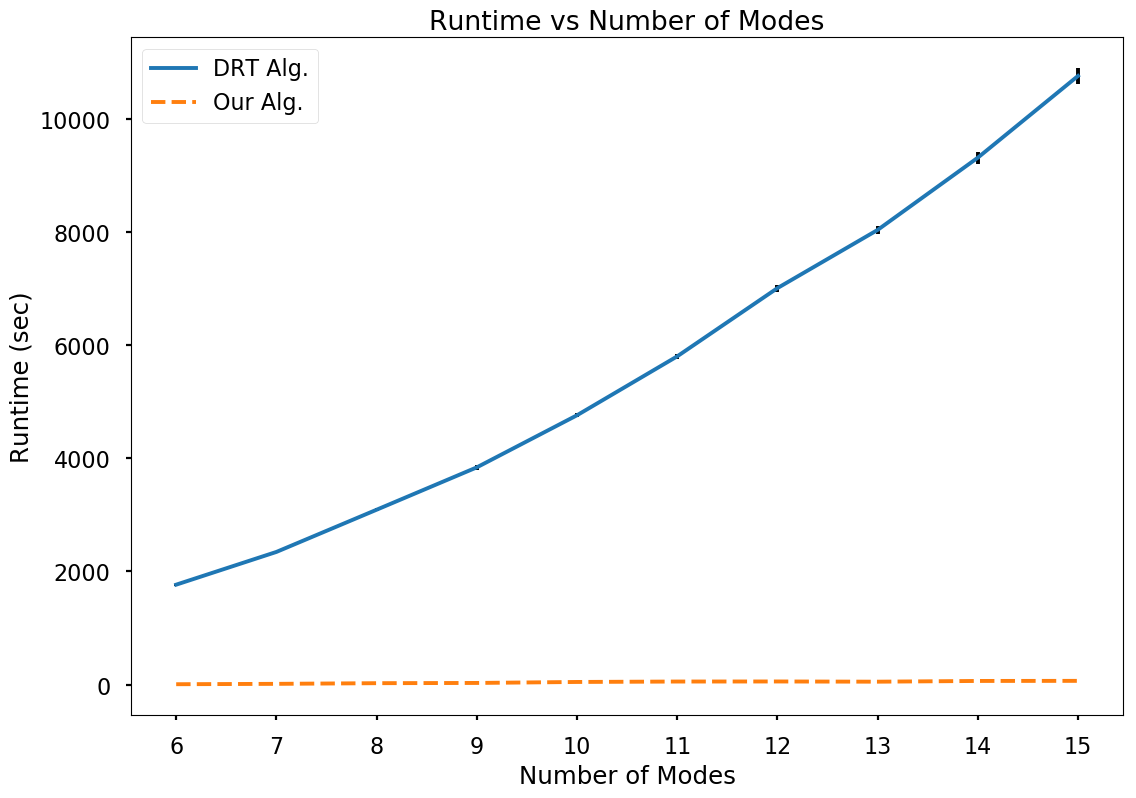
\includegraphics[width=1.0\linewidth]{fig/runtimePlot-confidence_intervals.png}
\caption{Runtime Comparison of Digraph Real-Time and Knapsack AVR Algorithm: Number of Modes}Graph depicting the runtime of different algorithms as a function of the number of modes of randomly generated AVR task sets. For each mode, the 95\% confidence interval is shown.
\label{fig:finalgraph}
\end{figure}

For the second experiment, we generated multiple AVR tasks using an algorithm presented by Biondi et al.~\cite{biondi_response-time_2015}. In this algorithm, multiple AVR tasks are modeled as a single task, called the representative AVR task, by combining the execution times and the boundaries speeds. The modes of the representative AVR task are generated by assuming a fixed value of 0.25 for the maximum utilization factor of the modes. Again, the same worst-case demands were found by both algorithm, but overall, our approach is 146 times faster on average and up to 250 times faster, as shown in Fig.~\ref{fig:finalgraph}.

%  \sandeep{This is how I calculated the confidence intervals and runtime averages:
%  For tasksets-1 and 2, run both the algorithms on each of the tasksets 10 times and calculate the average runtime of an algorithm per taskset. The improvement in runtime over a taskset is the ratio of the runtime average of the DRT algorithm on the given taskset and the runtime average of our algorithm on the same taskset. I do this because we have a table showing the average runtimes of our algorithm and the DRT algorithm over each of the tasksets.
%   For randomly generated tasksets: Generate 10 random tasksets each with modes 6 to 15. Run both the algorithms on each of these tasksets 10 times. Calculate the ratio of the runtime of the DRT algorithm over a taskset and the runtime of our algorithm for the corresponding run over the same taskset. The average of all the ratios (total number of averages will be 10*10=100 - each taskset has 10 averages) above gives the average improvement.
% The average runtimes and improvement ratios are calculated differently in the above two cases. Is this fine?}

\subsection{Conclusions and Future Work}
\label{sec:conclusion}

This paper presented an efficient method for calculating the exact worst-case demand bound function of AVR tasks. First, a knapsack-based dynamic programming approach was proposed to efficiently find the worst-case demand. Second, a collection of necessary conditions were presented, which reduce the search space of the knapsack-based approach to find the dominant sequence set. Experimental results confirm that the proposed approach is exact and is faster than the state-of-the-art technique. In the future, we plan on analyzing the worst-case demand of AVR tasks that have different phases and which are released by independent sources.

% Paper \# 1
% I <3 my Wayne State Libraries! Do you? \cite{WSULibrary}

% \paragraph{A Subsection with a Table}

% \begin{table}[!h]
%     \centering	
%     \bgroup
%     \def\arraystretch{1.00}
%     \begin{tabular}{| c | c | c | c |}
%           \hline			
%           Resource & Website & What's it for? \\ \hline \hline \cline{1-3}
%           Academic Success Center & https://success.wayne.edu/ & Academic Success!\\ \hline
%           Campus Health Center & http://health.wayne.edu/ & Health! \\ \hline
%           Writing Research and Technology Zone & http://www.clas.wayne.edu/writing/ & Writing Help!\\ \hline
%     \end{tabular}
%     \egroup
%     \caption{Wayne State University Resources}
%     \label{tab:WSUresources}
% \end{table}

% \paragraph{A Subsection with a Figure}

% \begin{figure}[!htbp]
%     \centering
%     
\includegraphics[width=0.25\linewidth]{fig/wsu_primary_stacked_color.pdf}
%     \caption{WSU Logo} The Wayne State University Logo
%     \label{fig:WSUlogo}
% \end{figure}

% \paragraph{A last Subsection}

\clearpage

%Compile Chapter N
\section{Future Work, Timeline, and Target Venues} \label{chap:futureWork}

In the previous chapters, two examples of real-time parameters directly connecting to real-world systems are covered.
These works provide a foundation upon which to extend current results.
This chapter covers proposed future works, a timeline for completion, and the target venues for publishing the work.

\subsection{Future Works}

As with the systems previously covered, these works focus on leveraging the interconnectedness of real-time parameters and physical systems to derive new or improved DBF calculations, utilization bounds, or codesign possibilities.
In practice, less pessimistic DBFs and utilization bounds increase schedulability.
Faster DBF and utilization bound algorithms make rescheduling online more feasible.

\subsubsection{DBF of Monotonically Ascending Execution Sequences}

The Generalized Multi-Frame Model (GMF) can be used to characterize the demand of a task with Repeating WCET Sequences (RWSs).
RWSs with Monotonically Ascending Execution times (MAEs), however, are not exploited by the GMF model.
The most applicable approach to computing a DBF for RWSs with MAEs is computationally expensive - $O(N^2 lg N)$.
Preliminary results on exploiting MAEs reduce the DBF to calculation to $O(N lg N)$ time.
Since $N$ is the number of WCETs in the RWS, this is a significant improvement over the state of the art.
In practice, this approach could be used for modeling systems in which number of sensors used in a control task increase as the system approaches a setpoint.
The aim of this work is to present a faster DBF calculation for tasks using RWSs with MAEs.
% The target contributions of this work include:
% \begin{enumerate}
%     \item a real-time task model for describing RWSs,
%     \item an algorithm for creating a DBF for a particular RWS, and 
%     \item a case study of calculating DBF for a robotic arm using a variable resolution ADC.
% \end{enumerate}

\subsubsection{DBF of Short Circuit Protection for Multiple Power Paths}

Our previous work focused on real-time short-circuit detection for single monitored power pathway using implicit deadlines\cite{willcock_trading_2017}.
A relationship between inductor size and real-time utilization under EDF was established to demonstrate tradeoff between board space consumed and real-time task utilization.
To further this work, short-circuit detection will be implemented on multiple, monitored power distribution pathways sharing a single source.
In practice, this approach would be implemented in power distribution panels where current monitoring is required.
The aim of this work is to present a tighter, less pessimistic bound on the utilization of real-time short-circuit protection tasks by leveraging maximum current through the single-source.
% Single-source power pathways, such as a battery supplying several loads or a breaker box in a house powering all receptacles, have maximum currents which are not equivalent to the sum of all individual power pathways' maximum current.
% For example, most home breakers allow a maximum of 100 or 200 Amperes of continuous current.
% Individual breakers allow a maximum of 15-30 Amperes of continuous current.
% Yet there are more than 10 breakers on a home breaker box.
% This is because not all pathways are expected to draw maximum current simultaneously.
% In real-time systems responsible for current monitoring and short-circuit protection of power distribution pathways, this limitation on maximum power from the common source can be exploited to limit the maximum utilization of all current monitoring tasks.
% The target contributions of this work include:
% \begin{enumerate}
%     \item a utilization bound on software-based short-circuit protection for $n$ monitored, single-source power pathways,
%     \item a demand bound function for software-based short-circuit protection for $n$ monitored, single-source power pathways,
%     \item a formal relationship between the DBF of the short-circuit protection tasks and the power path parameters (such as inductor size, max current, critical current, and single source current limit),
%     \item and a case study on a ~50A power distribution system for an autonomous ground vehicle.
% \end{enumerate}

\subsubsection{FPTAS for AVR Task DBF}

Our previous  work on demand characterization of AVR tasks in ICEs does not leverage any approximation \cite{bijinemula_efficient_2019}.
While exact, this characterization may not be suitable online where computing power and time are significantly constrained.
Systems which reallocate tasks across ECUs or change the transition speeds online \cite{peng_schedulability_2018} cannot afford the time or energy required by the exact approach benefit from an approximation alternative.
The aim of this work is to develop an FPTAS of the exact demand characterization presented in Bijinemula et al. \cite{bijinemula_efficient_2019}.

\subsubsection{DBF of AVR Tasks in ICEs with Dynamic-Skip Fire}

The demand characterization offered by the Knapsack AVR approach is for a single AVR task which corresponds to a single piston in an ICE \cite{bijinemula_efficient_2019}.
In practice, ICEs have more than one cylinder.
Increasing interest in efficient ICEs has driven manufacturers to produce ICEs capable of disabling fuel injection and/or changing the stroke length of individual cylinders.
These techniques, along with others not mentioned here, are referred to as Variable Displacement (VD) as they change the total displacement of the ICE.
VD techniques are used when engine load is low to conserve fuel and are disabled when engine load is high (under acceleration, for example).
If each cylinder is associated with an AVR task, and cylinders are disabled (or max acceleration reduced) during low loads, a proper demand characterization of the engine must have one task per cylinder and incorporate the effects of VD.
The aim of this work is to develop a DBF for AVR tasks in ICEs implementing VD through a strategy known as Dynamic Skip-Fire (DSF).
% The target contributions of this work include:
% \begin{enumerate}
%     \item a real-time task model for AVR tasks in ICEs implementing VD through the Dynamic Skip-Fire (DSF),
%     \item a set of transformations for reducing the search space for AVR tasks in ICEs with DSF, and
%     \item an exact DBF for a set of $Y$ AVR tasks implementing DSF on a $Y$-cylinder ICE.
% \end{enumerate}

\subsubsection{Online Demand-Based Hybrid Powertrain Reconfiguration}

Recent works like Badam et al. \cite{badam_software_2015} and He et al. \cite{he_case_2017} focus on the development of reconfigurable and software-defined batteries.
In Badam et al., cells of different chemistries (with varied advantages over each other) are toggled between to extend the life of the battery.
% The work illustrated how certain chemistries are better for short-term, high current draw while others are best suited for long-term, low current draw.
In He et al. \cite{he_case_2017}, batteries are shown to be capable of parallelizing or serializing individual cells to isolate failing cells from the battery power paths - preventing them from degrading the output of the entire battery.
% To extend in the direction of these works, we intend to develop strategies for route-responsive powertrain reconfiguration.
For electric and hybrid vehicles in which destinations are known a priori, public information like elevation change, intersections, and speed limits can provide projected power requirements for traveling a given route.
This projected power requirement can be translated to a demand profile for a hybrid powertrain.
In the case of reconfigurable batteries, the demand profile can be used parallelize or serialize cells online while traveling the route to minimize energy cost, extend battery life, or minimize travel time.
The aim of this work is to develop algorithms for reconfiguring a hybrid battery online to meet projected power requirements while minimizing the number of cells and total energy required.
% In the case of mixed-chemistry batteries, the demand profile can be used to prioritize chemistries during charging and map chemistries to segments of the route.
% In the case of a hybrid powertrain with an internal combustion engine and battery available for propulsion, the demand profile can be used to identify which source should supply propulsion over the route.
% The target contributions of this work include:
% \begin{enumerate}
%     \item a generic model of mixed-source powertrains,
%     \item algorithms for identifying legal powertrain configurations which meet projected power requirements,
%     \item algorithms for identifying charging (or refueling) priorities for minimizing energy consumption or cost of operation,
%     \item and a case study on a 
% \end{enumerate}

\subsection{Timeline and Target Venues}

Table \ref{tab:timeline} lists the timeline for the remaining expected publications.
The publication type, project name, and target venue are also provided.
Table \ref{tab:targetVenues} lists the full names and abbreviations of the target venues.

\begin{table}[h]
    \centering
    \def\arraystretch{1.25}%  1 is the default, change whatever you need
    \begin{tabular}{|l|l|l|l|l}
    \cline{1-4}
    \textbf{Target Date} & \textbf{Publication Type} & \textbf{Project}                                                                             & \textbf{Target Venue} &  \\ \cline{1-4}
    2021-03-03           & Conference                & \begin{tabular}[c]{@{}l@{}}WCD of Monotonically Ascending\\ Execution Sequences\end{tabular} & ECRTS                      &  \\ \cline{1-4}
    2021-04-01           & Journal                   & \begin{tabular}[c]{@{}l@{}}DBF of Short Circuit Protection\\ for Multiple Power Paths\end{tabular}        & IEEE ToC                   &  \\ \cline{1-4}
    2021-05-01           & Journal                   & FPTAS for AVR Task DBF                                                                       & IEEE ToC                   &  \\ \cline{1-4}
    2021-05-25           & Conference                & \begin{tabular}[c]{@{}l@{}}DBF of AVR Tasks in ICEs\\ with Dynamic-Skip Fire\end{tabular}    & RTSS                       &  \\ \cline{1-4}
    2021-10-26           & Conference                & \begin{tabular}[c]{@{}l@{}}Online Demand-Based\\ Battery Reconfiguration\end{tabular}        & RTAS                       &  \\ \cline{1-4}
    \end{tabular}
    \caption{Target Publication Timeline}
    \label{tab:timeline}
\end{table}

\begin{table}[h]
    \centering
    \def\arraystretch{1.25}%  1 is the default, change whatever you need
    \begin{tabular}{|l|l|l|l}
    \cline{1-3}
    \textbf{Abbreviation} & \textbf{Type} & \textbf{Full Name}                                           &  \\ \cline{1-3}
    ECRTS                 & Conference    & Euromicro Conference on Real-Time Systems                    &  \\ \cline{1-3}
    RTSS                  & Conference    & Real-Time Systems Symposium                                  &  \\ \cline{1-3}
    RTAS                  & Conference    & \begin{tabular}[c]{@{}l@{}}Real-Time and Embedded Technology\\ and Applications Symposium\end{tabular} &  \\ \cline{1-3}
    IEEE ToC              & Journal       & IEEE Transactions on Computers                               &  \\ \cline{1-3}
    \end{tabular}
    \caption{Target Venues}
    \label{tab:targetVenues}
\end{table}
\clearpage

%Compile Chapter N
\section{Conclusion}   \label{chap:conclusion}

Autonomous vehicles, cyber physical systems, edge computing, internet of things, and smart infrastructure are the frontier of modern computing.
The success of applications in each of these domains rests upon correct and timely execution by processors and microcontrollers alike.
As hardware and software become ever more integrated, providing real-time guarantees becomes increasingly complicated.
Fortunately, this integration provides as many opportunities as it does challenges.
In this work, we address several ways in which the connection between physical system dynamics, like current and engine speed, and real-time task parameters, like WCET and interarrival time, can be leveraged to reduce the complexity of demand characterization and schedulability analysis.
This work also highlights how the connections between physical and real-time systems can be used for codesign and, most importantly, to allow advancements at either end of the relationship to benefit the other.
\clearpage

%Compile Chapter N
\section{Publication List}   \label{chap:publicationList}
\clearpage

%Appendices

%Compile Appendix A
\centerline{\large\bf APPENDIX A: Short Circuit Detection Materials}\label{appendix:scd-materials}
\addcontentsline{toc}{section}{Appendix A: Short Circuit Detection Materials}
Non-trivial materials used in the experiments can be found in Figure \ref{fig:Materials}. Excluded from the materials list are elements including cooper wire, breadboards, and a power supply. To minimize cost of replication, through-hole parts are used in place of smaller, surface-mount components.
\begin{figure}[!htbp]
    \centering	
    \bgroup
    \def\arraystretch{1.25}%  1 is the default, change whatever you need
    \begin{tabular}{| c | c | c |}
        \hline			
        Item & Manufacturer & Part Number(s)\\ \hline \hline \cline{1-3}
        Debugger & Microchip & PG164130\\ \hline
        Inductor & Triad Magnetics & RC-1; RC-2; RC-3\\ \hline
        Microprocessor & Microchip & DM164130-4\\ \hline
        Oscilloscope & RIGOL & DS1102E\\ \hline
        Oscilloscope Probe & HANTEK & PP-150\\  \hline  
        Power Resistor & YAGEO & 1334 10W 10R J\\  \hline  
        Resistor & N/A & 510$\Omega$ 5\% resistor\\  \hline  
    \end{tabular}
    \egroup
    \caption{Materials List}Materials list for Experiments 1-4
    \label{fig:Materials}
\end{figure}
\clearpage

%Compile Appendix B
%Create appendix with unnumbered section
\section*{APPENDIX B}
%Add appendix to toc at section level
\addcontentsline{toc}{section}{Appendix B}
\appendix{More Stuff and Things}\label{appendix:moreStuffAndThings}
My Appendix B...
\clearpage

%Compile Appendix C

\centerline{\large\bf APPENDIX C}
\addcontentsline{toc}{section}{Appendix C}

\appendix{Engine Control Appendix}\label{appendix:engineControl}

\subsection{Proof of Property~\ref{prop:high-speed-transfer}}
The property is restated here for readability.

\emph{Property 9 (Highest-Speed Relative-Deadline Dominance):}
For any valid, finite sequence $S = (\omega_1, \ldots, \omega_n)$, if $\omega_\ell$ ($\ell \in \mathbb{N}_1^n-1$) is the highest speed $s_n$ and not the last speed of sequence $S$ and $s_n \leq \Omega_1(\omega_n,\alpha_{\max})$ then new sequence $S'$ with the highest element moved to the last element (i.e., $S' = (\omega_1, \ldots, \omega_{\ell-1}, \omega_{\ell+1}, \ldots, \omega_n, s_n)$) is valid and has the following property: 
\begin{equation}\label{eqn:high-speed-transfer-appendix}
    d(S) \geq d(S').
\end{equation}


%%%%%%%%%%%%%%%%%%BEGIN COMMENT%%%%%%%%%%%%%%%%%%%%
% \begin{comment}

% \begin{IEEEproof} 
% Consider valid, finite sequence $S = (\omega_1, \ldots, \omega_n)$, where $\omega_\ell$ ($\ell \in \mathbb{N}_1^n-1$) is the highest speed $s_n$ and not the last speed of sequence $S$ and $s_n \leq \Omega_1(\omega_n,\alpha_{\max})$.

% Let $S$ be constructed as described in the statement of the lemma:  $S' = (\omega_1, \ldots, \omega_{\ell-1}, \omega_{\ell+1}, \ldots, \omega_n, s_n)$.  Observe that $S'$ is valid since $s_n$ is reachable from $\omega_n$; also, since $\Omega_1(\omega_{\ell-1},\alpha_{\max}) \geq s_n \geq \omega_{\ell-1}$ and $\Omega_1(\omega_{\ell+1},\alpha_{\max}) \geq s_n \geq \omega_{\ell+1}$, which implies that $\omega_{\ell-1}$ and $\omega_{\ell+1}$ are reachable from each other.  

% We define $\Delta_H(S,S')$ to be the difference $d(S) - d(S')$:
% \begin{equation}\label{eq:tHST}
% \begin{array}{ll}
%     \Delta_H(S,S') =& \widetilde{T}(\omega_{\ell-1}, s_n) + \widetilde{T}(s_n, \omega_{\ell+1})+  \Tilde{d}(\omega_n)\\
%      &- \widetilde{T}(\omega_{\ell-1},\omega_{\ell+1}) - \widetilde{T}(\omega_n, s_n)
%         - \Tilde{d}(s_n). 
% \end{array}
% \end{equation}

% We now prove that $\Delta_H(S,S') \geq 0$ which proves Equation~\ref{eqn:high-speed-transfer} of the property.  Let $s_{n-1}$ be the second largest speed of $S$.  By the partial derivatives of $\widetilde{T}$ in Equations~\ref{eq:minTimeDerivativeWrtInitial} and~\ref{eq:minTimeDerivativeWrtFinal}, for all $\epsilon > 0$
% \begin{equation}
%     \widetilde{T}(\omega_{\ell-1}, s_{n-1} +\epsilon) \geq
%     \widetilde{T}(s_{n-1}, s_{n-1} + \epsilon),
% \end{equation}
% \noindent since $s_{n-1} \geq \omega_{\ell-1}$.  Thus,
% \begin{equation}
% \begin{array}{ll}
%         \lefteqn{\widetilde{T}(\omega_{\ell-1}, s_{n-1}) + \widetilde{T}(\omega_{\ell-1}, s_{n-1} +\epsilon)}&\\
%         &\geq
%     \widetilde{T}(s_{n-1}, s_{n-1} + \epsilon) + \widetilde{T}(s_{n-1}, s_{n-1}).
% \end{array}
% \end{equation}

% Without loss of generality assume that $\omega_{\ell-1}\leq \omega_{\ell+1}$.  Letting $\epsilon = s_n - s_{n-1}$, we get
% \begin{equation}
% \begin{array}{ll}

%     &\begin{array}{ll}
%         \lefteqn{\widetilde{T}(\omega_{\ell-1}, s_{n-1}) + \widetilde{T}(\omega_{\ell-1}, s_{n})}&\\
%             &\geq
%         \widetilde{T}(s_{n-1}, s_{n}) + \widetilde{T}(\omega_{\ell+1}, s_{n-1})
%         \end{array}\\
%     \Rightarrow & \begin{array}{ll}
%         \lefteqn{\widetilde{T}(\omega_{\ell-1}, s_{n-1}) + \widetilde{T}(\omega_{\ell-1}, s_{n})}&\\
%             &\geq
%         \widetilde{T}(s_{n-1}, s_{n}) + \widetilde{T}(s_{n-1}, s_{n-1}).
%         \end{array}
% \end{array}
% \end{equation}
% Using the same reasoning from Equations~\ref{eq:minTimeDerivativeWrtInitial} and~\ref{eq:minTimeDerivativeWrtFinal},
% we can symmetrically show that
% \begin{equation}
% \begin{array}{ll}

%      & \begin{array}{ll}
%         \lefteqn{\widetilde{T}(\omega_{\ell-1}, s_{n}) + \widetilde{T}(\omega_{\ell-1}, s_{n})}&\\
%             &\geq
%         \widetilde{T}(s_{n-1}, s_{n}) + \widetilde{T}(s_{n-1}, s_{n-1})
%         \end{array}
% \end{array}
% \end{equation}


% \begin{alignat}{4}
% && \widetilde{T}(q_k, \omega_k) + \widetilde{T}(\omega_k,\omega_{k+1}) & \leq \widetilde{T}(\omega_k,\omega_k) + \widetilde{T}(q_k,\omega_{k+1}) && \nonumber \\
% && & \qquad \qquad \qquad \quad \quad \text{By Eq. \ref{eq:HSTcomp}} \nonumber \\
% \Leftrightarrow && \widetilde{T}(q_k, \omega_k) + \widetilde{T}(\omega_k,\omega_{k+1}) & \leq \widetilde{T}(q_x,\omega_k) + \widetilde{T}(q_k,\omega_{k+1}) & \quad & \nonumber \\
% \Leftrightarrow && \widetilde{T}(q_n, \omega_n) + \widetilde{T}(\omega_k,\omega_{k+1}) & \leq \widetilde{T}(q_{x},\omega_n) + \widetilde{T}(\omega_n,q_{x+2}) && \nonumber \\
% && & \quad + \widetilde{T}(q_k,\omega_{k+1}) \quad \text{By Eq. \ref{eq:minimumTimeNonNegative}}& \nonumber \\
% %\Leftrightarrow && \widetilde{T}(q_k, \omega_k) + E(\omega_k) - (\widetilde{T}(q_{x},\omega_k) + \widetilde{T}(\omega_k,q_{x+2}) + E(q_k)) & \leq 0 & \nonumber \\
% \Leftrightarrow && \Delta t_{HST}(Q(S(k)) & \leq 0 &\quad&
% \end{alignat}


% \begin{alignat}{3}\label{eq:tHST}
% &\Delta_H(S) =&\nonumber \\
% &\left\{
%     \def\arraystretch{1.0}
%     \begin{array}{ll}
%         \widetilde{T}(s_n, \omega_n) + \Tilde{d}(\omega_n)\\
%         - (\widetilde{T}(\omega_n,q_2) + \Tilde{d}(q_k)) & \quad k = n, q_1 = \omega_k\\
%         \widetilde{T}(q_k, \omega_k) + \widetilde{T}(\omega_k,\omega_{k+1})\\
%         - (\widetilde{T}(\omega_k,q_2) + \widetilde{T}(q_k,\omega_{k+1})) & \quad k < n, q_1 = \omega_k \\
%         \widetilde{T}(q_n, \omega_n) + \Tilde{d}(\omega_n) - (\widetilde{T}(q_x,\omega_n)\\
%         + \widetilde{T}(\omega_n,q_{x+2}) + \Tilde{d}(q_n)) & \quad k = n, q_{x+1} = \omega_k\\
%         \widetilde{T}(q_k, \omega_k) + \widetilde{T}(\omega_k,\omega_{k+1})\\
%         - (\widetilde{T}(q_x,\omega_k) + \widetilde{T}(\omega_k,q_{x+2})\\
%         + \widetilde{T}(q_k,\omega_{k+1}) & \quad k < n, q_{x+1} = \omega_k
%     \end{array}
% \right.
% \end{alignat}

% We now prove the time-reducing property of Equation \ref{eq:tHST}:
% \begin{property}[High Speed Transfer Time Reduction]\label{lem:HST}
% $\forall Q(S(k))$, $\Delta t_{LHST}(Q(S(k)) \leq 0$.
% \end{property}
% \begin{IEEEproof}
% Suppose that $k = n, q_1 = \omega_k$. Given $\widetilde{T}(\omega,f) + E(\omega)$, let $\omega = q_n$, $f = \omega_n$, and $\delta = \omega_n - q_n$. Comparing the partial increase $\delta$ on either $\omega$ term gives:
% \begin{alignat}{4}
% && \widetilde{T}(\omega,f) + E(\omega) & = \widetilde{T}(\omega,f) + E(\omega) \nonumber\\
% \Leftrightarrow && \widetilde{T}(q_n, \omega_n) + E(q_n) & = \widetilde{T}(q_n,\omega_n) + E(q_n) && \nonumber \\
% \Leftrightarrow && \widetilde{T}(q_n, \omega_n) + E(q_n+\delta) & \leq \widetilde{T}(q_n+\delta,\omega_n) + E(q_n) &&\nonumber \\
% &&& \quad \text{By Eq.  \ref{eq:partialEpartialwCompare}} \nonumber \\
% \Leftrightarrow && \widetilde{T}(q_n, \omega_n) + E(\omega_n) & \leq \widetilde{T}(\omega_n,\omega_n) + E(q_n) && \label{eq:HSETcomp}\\
% \Leftrightarrow && \widetilde{T}(q_n, \omega_n) + E(\omega_n) & \leq \widetilde{T}(\omega_n,q_2) + E(q_n) && \nonumber \\
% %\Leftrightarrow && \widetilde{T}(q_k, \omega_k) + E(\omega_k) - (\widetilde{T}(\omega_k,q_2) + E(q_k)) & \leq 0 & \nonumber \\
% \Leftrightarrow && \Delta t_{HST}(Q(S(k)) & \leq 0 \quad \text{By Eq. \ref{eq:tHST}} &&\nonumber
% \end{alignat}
% Suppose now that $k < n, q_1 = \omega_k$. Given $\widetilde{T}(\omega,f) + E(\omega)$, let $\omega = q_k$, $f_1 = \omega_k$, $f_2 = \omega_{k+1}$ and $\delta = \omega_k - q_k$. Comparing the partial increase $\delta$ on either $\omega$ term gives:
% \begin{alignat}{4}
% && \widetilde{T}(\omega,f_1) + \widetilde{T}(\omega,f_2) & = \widetilde{T}(\omega,f_1) + \widetilde{T}(\omega,f_2) \nonumber\\
% \Leftrightarrow && \widetilde{T}(q_k, \omega_k) + \widetilde{T}(\omega_k,\omega_{k+1}) & = \widetilde{T}(q_k,\omega_k) + \widetilde{T}(\omega_k,\omega_{k+1}) &\quad& \nonumber \\
% \Leftrightarrow && \widetilde{T}(q_k, \omega_k) + \widetilde{T}(q_k+\delta,\omega_{k+1}) & \leq \widetilde{T}(q_k+\delta,\omega_k) &\quad& \nonumber \\
% && & \quad + \widetilde{T}(q_k,\omega_{k+1}) \: \text{By Eq.  \ref{eq:minTimeDerivativeWrtInitial}} \nonumber \\
% \Leftrightarrow && \widetilde{T}(q_k, \omega_k) + \widetilde{T}(\omega_k,\omega_{k+1}) & \leq \widetilde{T}(\omega_k,\omega_k) + \widetilde{T}(q_k,\omega_{k+1}) &\quad& \label{eq:HSTcomp}\\
% \Leftrightarrow && \widetilde{T}(q_k, \omega_k) + \widetilde{T}(\omega_k,\omega_{k+1}) & \leq \widetilde{T}(\omega_k,q_2) + \widetilde{T}(q_k,\omega_{k+1}) && \nonumber \\
% %\Leftrightarrow && \widetilde{T}(q_k, \omega_k) + E(\omega_k) - (\widetilde{T}(\omega_k,q_2) + E(q_k)) & \leq 0 & \nonumber \\
% \Leftrightarrow && \Delta t_{HST}(Q(S(k)) & \leq 0 \quad \text{By Eq. \ref{eq:tHST}} &&
% \end{alignat}
% Suppose now that $k = n, q_{x+1} = \omega_k$. Consider now that for $\omega_k$ to be the highest speed, $q_x$ and $q_{x+2}$ in Equation \ref{eq:HST} are no greater than $\omega_k$. Using the assumptions from the IEEEproof of Lemma \ref{lem:HST}, Equation \ref{eq:HSTcomp} serves as a base inequality for comparison:
% \begin{alignat}{4}
% && \widetilde{T}(q_n, \omega_n) + E(\omega_n) & \leq \widetilde{T}(\omega_n,\omega_n) + E(q_n) & \text{By Eq. \ref{eq:HSETcomp}} \nonumber \\
% \Leftrightarrow && \widetilde{T}(q_n, \omega_n) + E(\omega_n) & \leq \widetilde{T}(\omega_n,q_{x+2}) + E(q_n) &\quad& \nonumber \\
% \Leftrightarrow && \widetilde{T}(q_n, \omega_n) + E(\omega_n) & \leq \widetilde{T}(q_{x},\omega_n) + \widetilde{T}(\omega_n,q_{x+2}) && \nonumber \\
% && & \quad + E(q_n) \quad \text{By Eq. \ref{eq:minimumTimeNonNegative}} \nonumber \\
% %\Leftrightarrow && \widetilde{T}(q_k, \omega_k) + E(\omega_k) - (\widetilde{T}(q_{x},\omega_k) + \widetilde{T}(\omega_k,q_{x+2}) + E(q_k)) & \leq 0 & \nonumber \\
% \Leftrightarrow && \Delta t_{HST}(Q(S(k)) & \leq 0
% \end{alignat}
% Finally, suppose that $k < n, q_{x+1} = \omega_k$. Recall for $\omega_k$ to be the highest speed, $q_x$ and $q_{x+2}$ in Equation \ref{eq:HST} are no greater than $\omega_k$. Equation \ref{eq:HSTcomp} serves as a base inequality for comparison:
% \begin{alignat}{4}
% %\Leftrightarrow && \widetilde{T}(q_n, \omega_n) + E(\omega_n) & \leq \widetilde{T}(\omega_n,q_{x+2}) + E(q_n) &\quad& \nonumber \\
% %\Leftrightarrow && \widetilde{T}(q_n, \omega_n) + E(\omega_n) & \leq \widetilde{T}(q_{x},\omega_n) + \widetilde{T}(\omega_n,q_{x+2}) + E(q_n) &\quad& \text{By Eq. \ref{eq:minimumTimeLessThanZeroHighF}, \ref{eq:minimumTimeLessThanZeroLowF}} \nonumber \\
% && \widetilde{T}(q_k, \omega_k) + \widetilde{T}(\omega_k,\omega_{k+1}) & \leq \widetilde{T}(\omega_k,\omega_k) + \widetilde{T}(q_k,\omega_{k+1}) && \nonumber \\
% && & \qquad \qquad \qquad \quad \quad \text{By Eq. \ref{eq:HSTcomp}} \nonumber \\
% \Leftrightarrow && \widetilde{T}(q_k, \omega_k) + \widetilde{T}(\omega_k,\omega_{k+1}) & \leq \widetilde{T}(q_x,\omega_k) + \widetilde{T}(q_k,\omega_{k+1}) & \quad & \nonumber \\
% \Leftrightarrow && \widetilde{T}(q_n, \omega_n) + \widetilde{T}(\omega_k,\omega_{k+1}) & \leq \widetilde{T}(q_{x},\omega_n) + \widetilde{T}(\omega_n,q_{x+2}) && \nonumber \\
% && & \quad + \widetilde{T}(q_k,\omega_{k+1}) \quad \text{By Eq. \ref{eq:minimumTimeNonNegative}}& \nonumber \\
% %\Leftrightarrow && \widetilde{T}(q_k, \omega_k) + E(\omega_k) - (\widetilde{T}(q_{x},\omega_k) + \widetilde{T}(\omega_k,q_{x+2}) + E(q_k)) & \leq 0 & \nonumber \\
% \Leftrightarrow && \Delta t_{HST}(Q(S(k)) & \leq 0 &\quad&
% \end{alignat}
% Thus, Equation \ref{eq:HST} implies that any sequence $Q(\mathcal{S}(k)) \in \mathcal{Q}_{feasible}$ with highest speed job $q_i = \omega_k$ where $1 \leq i < k$ can be transformed into $Q'(\mathcal{S}(k))$ with $\omega_k$ as the final job such that $\Delta_t(Q'(\mathcal{S}(k))) \leq \Delta_t(Q(\mathcal{S}(k))$.
% \end{IEEEproof}

% \end{comment}
%%%%%%%%%%%%%%%%%%%%%END COMMENT%%%%%%%%%%%%%%%%%%%%%%


\begin{proof}
Consider a valid, finite sequence $S = (\omega_1, \ldots, \omega_n)$, where $\omega_\ell$ ($\ell \in \mathbb{N}_1^n-1$) is the highest speed $s_n$ and not the last speed of sequence $S$ and $s_n \leq \Omega_1(\omega_n,\alpha_{\max})$.

Let $S$ be constructed as described in the statement of the lemma:  $S' = (\omega_1, \ldots, \omega_{\ell-1}, \omega_{\ell+1}, \ldots, \omega_n, s_n)$.  Observe that $S'$ is valid since $s_n$ is reachable from $\omega_n$; also, since $\Omega_1(\omega_{\ell-1},\alpha_{\max}) \geq s_n \geq \omega_{\ell-1}$ and $\Omega_1(\omega_{\ell+1},\alpha_{\max}) \geq s_n \geq \omega_{\ell+1}$, which implies that $\omega_{\ell-1}$ and $\omega_{\ell+1}$ are reachable from each other.  

We define $\Delta_H(S,S')$ to be the difference $d(S) - d(S')$:
\begin{equation}\label{eq:tHST}
\begin{array}{ll}
    \Delta_H(S,S') =& \widetilde{T}(\omega_{\ell-1}, s_n) + \widetilde{T}(s_n, \omega_{\ell+1})+  \Tilde{d}(\omega_n)\\
     &- \widetilde{T}(\omega_{\ell-1},\omega_{\ell+1}) - \widetilde{T}(\omega_n, s_n)
        - \Tilde{d}(s_n). 
\end{array}
\end{equation}

We now prove that $\Delta_H(S,S') \geq 0$ which proves Equation~\ref{eqn:high-speed-transfer-appendix} of the property.  Let $s_{n-1}$ and $s_{n-2}$ be the second and third largest speed of $S$, respectively.

The rest of the proof is nearly identical to Property~\ref{prop:ascending-dominates-I}.
Observe that by Properties~\ref{T-reversal} and~\ref{prop:deadline-derivative}, $\widetilde{T}(f,\omega + \epsilon) \geq \tilde{d}(\omega + \epsilon)$ for all $f, \omega$ and $\epsilon > 0$.  Also, $\widetilde{T}(s_k +\epsilon, \omega) = \widetilde{T}(\omega, s_k+\epsilon)$ for all $\omega$ and $\epsilon >0$ by Property~\ref{T-reversal}.  These properties imply that:
\begin{equation}\label{eqn:change-sn}
\begin{array}{ll}
     & 
     \begin{array}{ll}
        \lefteqn{\widetilde{T}(s_{n-2},s_{n-1}) + \widetilde{T}(s_{n-1}, s_{n-1}) + \tilde{d}(s_{n-1})}& \\
            &= \widetilde{T}(s_{n-2},s_{n-1}) + \widetilde{T}(s_{n-1},s_{n-1}) + \tilde{d}(s_{n-1})
      \end{array}\\
     \Rightarrow & 
     \begin{array}{ll}
        \lefteqn{\widetilde{T}(s_{n-2},s_{n-1} +\epsilon) + \widetilde{T}(s_{n-1}+\epsilon, s_{n-1}) + \tilde{d}(s_{n-1})}& \\
        &\geq \widetilde{T}(s_{n-2},s_{n-1}) + \widetilde{T}(s_{n-1}, s_{n-1} + \epsilon) + \tilde{d}(s_{n-1}+\epsilon) 
    \end{array}\\
\end{array}
\end{equation}

\noindent Setting $\epsilon = s_{n} - s_{n-1}$ and substituting into the above inequality of Equation~\ref{eqn:change-sn}, we get the following:
\begin{equation}\label{eqn:change-sn2}
\begin{array}{ll}
     &\begin{array}{ll}
        \lefteqn{\widetilde{T}(s_{n-2},s_{n}) + \widetilde{T}(s_{n}, s_{n-1}) + \tilde{d}(s_{n-1})}& \\
        &\geq \widetilde{T}(s_{n-2},s_{n-1}) + \widetilde{T}(s_{n-1}, s_{n}) + \tilde{d}(s_{n}) 
    \end{array}\\
    \Rightarrow&
    \begin{array}{ll}
        \lefteqn{\widetilde{T}(s_{n-2},s_{n}) + \widetilde{T}(s_{n}, s_{n-1}) - \widetilde{T}(s_{n-2},s_{n-1})}& \\
        &\geq \widetilde{T}(s_{n-1}, s_{n}) + \tilde{d}(s_{n}) - \tilde{d}(s_{n-1})
    \end{array}\\
\end{array}
\end{equation}

Seeing that both $\omega_{\ell-1}$ and $\omega_{\ell+1}$ are at most $s_{n-1}$ and either one of $\omega_{\ell-1}$ and $\omega_{\ell+1}$  must be less than $s_{n-2}$, we get:
\begin{equation}
\begin{array}{ll}
    \lefteqn{\widetilde{T}(\omega_{\ell-1}, s_n)  +\widetilde{T}(s_n,\omega_{\ell+1}) + \tilde{d}(\omega_n)} &\\
    &- \widetilde{T}(\omega_{\ell-1},\omega_{\ell+1}) - \widetilde{T}(\omega_n, s_{n})  - \tilde{d}(s_n) \geq 0
\end{array}
\end{equation}

\noindent The last inequality (which implies Equation~\ref{eq:tHST} of the property) above follows from observing that according to Property~\ref{prop:neg-deriv-min-interarrival}, the following is true for all $\omega$ and $\omega'$:
\begin{equation}
\begin{array}{ll}
        &\frac{\partial \widetilde{T}(\omega,s_{k+1})}{\partial \omega}
            \leq \frac{\partial \widetilde{T}(\omega,\omega')}{\partial \omega} \nonumber\\
        \Leftrightarrow&
        \frac{\partial \widetilde{T}(\omega,s_{k+1})}{\partial \omega} + \frac{\partial \widetilde{T}(s_{k+1},\omega')}{\partial \omega} - \frac{\partial \widetilde{T}(\omega,\omega')}{\partial \omega} \leq 0 \nonumber  
\end{array}
\end{equation}
\end{proof}

\subsection{Table of Notation and Units} \label{appendix:table-of-notation}

\begin{center}
\bgroup
\def\arraystretch{1.25}%
\resizebox{\linewidth}{!}{%
\begin{tabular}{| c | l | c | c |}
    
    \hline			
    Symbol & Term & Unit \\  \hline \hline \cline{1-3}
    $\omega$ & Angular speed & rev/min \\ \cline{1-3}
    $\omega_{rb}$ & Right boundary speed & rev/min \\ \cline{1-3}
    $\mathbf{\Omega_{rb}}$ & Set of right boundary speeds & N/A \\ \cline{1-3}
    $\omega_{\max}$ & Maximum angular velocity & rev/min \\ \cline{1-3}
    $\alpha$ & Angular acceleration & rev/$\text{min}^2$ \\ \cline{1-3}
    $\alpha_{\max}$ & Maximum angular acceleration & rev/$\text{min}^2$ \\ \cline{1-3}
    $\alpha_{\min}$ & Minimum angular acceleration & rev/$\text{min}^2$ \\ \cline{1-3}
    $t$ & Time & sec. \\ \cline{1-3}
    $\omega(t)$ & Instantaneous angular velocity & rev/min \\ \cline{1-3}
    $c(\omega(t))$ & Worst-case execution time & sec. \\ \cline{1-3}
    $\theta$ & Angular position & rev \\ \cline{1-3}
    $\Delta \theta$ & Change in angular distance & rev \\ \cline{1-3}
    $\Omega_n$ & Angular velocity at the end of `n' rotations & rev/min \\ \cline{1-3}
    $\tilde{T}$ & Minimum interarrival time & sec. \\ \cline{1-3}
    $\omega_p$ & Peak angular velocity & rev/min \\ \cline{1-3}
    $f$ & Angular velocity at the end of a rotation & rev/min \\ \cline{1-3}
    %$\omega_p(\omega,f)$ & Peak Angular Velocity & rev/min \\ \cline{1-3}
    $d(\omega)$ & Relative deadline & sec. \\ \cline{1-3}
    $D_\omega$ & Demand & sec. \\ \cline{1-3}
    $\dbf$ & Demand Bound Function & sec. \\ \cline{1-3}
    $\delta$ & Time interval length & sec. \\ \cline{1-3}
    $\mathbb{N}_j^k$ & Number set ${j, j+1, ... , k}$& N/A \\ \cline{1-3}
    $G_I$ & Dependency graph & N/A \\ \cline{1-3}
    $V_I$ & Vertices & N/A \\ \cline{1-3}
    $A_I$ & Edges & N/A \\ \cline{1-3}
    $\eta$ & Number of job releases & N/A \\ \cline{1-3}
    $\mathbb{Z}^+$ & Positive integers & N/A \\ \cline{1-3}
    $S$ & Speed sequence & N/A \\ \cline{1-3}
    $s_i$ & Job release speed & rev/min \\ \cline{1-3}
%    $S_A$ & Ascending Speed Sequence & UNIT \\ \cline{1-3}
%    $S(k)$ & Lowest k Speeds in Speed Sequence S & UNIT \\ \cline{1-3}
    $\Delta_L$ & Leading injection & N/A \\ \cline{1-3}
    $\Delta_F$ & Final injection & N/A \\ \cline{1-3}
    $\Delta_I$ & Internal injection & N/A \\ \cline{1-3}
    \hline  
\end{tabular}}
\egroup
\end{center}
\clearpage

%Compile Appendix D

\centerline{\large\bf APPENDIX D: Engine Control - Table of Notation and Units}
\addcontentsline{toc}{section}{Appendix C: Engine Control - Table of Notation and Units}\label{appendix:engCtrl-table-of-notation}

\begin{center}
\bgroup
\begin{tabular}{| c | l | c | c |}
    
    \hline			
    Symbol & Term & Unit \\  \hline \hline \cline{1-3}
    $\omega$ & Angular speed & rev/min \\ \cline{1-3}
    $\omega_{rb}$ & Right boundary speed & rev/min \\ \cline{1-3}
    $\mathbf{\Omega_{rb}}$ & Set of right boundary speeds & N/A \\ \cline{1-3}
    $\omega_{\max}$ & Maximum angular velocity & rev/min \\ \cline{1-3}
    $\alpha$ & Angular acceleration & rev/$\text{min}^2$ \\ \cline{1-3}
    $\alpha_{\max}$ & Maximum angular acceleration & rev/$\text{min}^2$ \\ \cline{1-3}
    $\alpha_{\min}$ & Minimum angular acceleration & rev/$\text{min}^2$ \\ \cline{1-3}
    $t$ & Time & sec. \\ \cline{1-3}
    $\omega(t)$ & Instantaneous angular velocity & rev/min \\ \cline{1-3}
    $c(\omega(t))$ & Worst-case execution time & sec. \\ \cline{1-3}
    $\theta$ & Angular position & rev \\ \cline{1-3}
    $\Delta \theta$ & Change in angular distance & rev \\ \cline{1-3}
    $\Omega_n$ & Angular velocity at the end of `n' rotations & rev/min \\ \cline{1-3}
    $\tilde{T}$ & Minimum interarrival time & sec. \\ \cline{1-3}
    $\omega_p$ & Peak angular velocity & rev/min \\ \cline{1-3}
    $f$ & Angular velocity at the end of a rotation & rev/min \\ \cline{1-3}
    %$\omega_p(\omega,f)$ & Peak Angular Velocity & rev/min \\ \cline{1-3}
    $d(\omega)$ & Relative deadline & sec. \\ \cline{1-3}
    $D_\omega$ & Demand & sec. \\ \cline{1-3}
    $\dbf$ & Demand Bound Function & sec. \\ \cline{1-3}
    $\delta$ & Time interval length & sec. \\ \cline{1-3}
    $\mathbb{N}_j^k$ & Number set ${j, j+1, ... , k}$& N/A \\ \cline{1-3}
    \hline  
\end{tabular}
\egroup
\end{center}

\begin{center}
\bgroup
\begin{tabular}{| c | l | c | c |}
    \hline
    Symbol & Term & Unit \\  \hline \hline \cline{1-3}
    $G_I$ & Dependency graph & N/A \\ \cline{1-3}
    $V_I$ & Vertices & N/A \\ \cline{1-3}
    $A_I$ & Edges & N/A \\ \cline{1-3}
    $\eta$ & Number of job releases & N/A \\ \cline{1-3}
    $\mathbb{Z}^+$ & Positive integers & N/A \\ \cline{1-3}
    $S$ & Speed sequence & N/A \\ \cline{1-3}
    $s_i$ & Job release speed & rev/min \\ \cline{1-3}
%    $S_A$ & Ascending Speed Sequence & UNIT \\ \cline{1-3}
%    $S(k)$ & Lowest k Speeds in Speed Sequence S & UNIT \\ \cline{1-3}
    $\Delta_L$ & Leading injection & N/A \\ \cline{1-3}
    $\Delta_F$ & Final injection & N/A \\ \cline{1-3}
    $\Delta_I$ & Internal injection & N/A \\ \cline{1-3}
\end{tabular}
\egroup
\end{center}
\clearpage

%Compile Appendix E

\centerline{\large\bf APPENDIX E: Short Circuit Detection - Table of Notation and Units}
\addcontentsline{toc}{section}{Appendix E: Short Circuit Detection - Table of Notation and Units}\label{appendix:scd-table-of-notation}
\begin{center}
\bgroup
\begin{tabular}{| c | l | c | c |}
    \hline
    Symbol & Term & Unit \\  \hline \hline \cline{1-3}
    $G_I$ & Dependency graph & N/A \\ \cline{1-3}
    $V_I$ & Vertices & N/A \\ \cline{1-3}
    $A_I$ & Edges & N/A \\ \cline{1-3}
    $\eta$ & Number of job releases & N/A \\ \cline{1-3}
    $\mathbb{Z}^+$ & Positive integers & N/A \\ \cline{1-3}
    $S$ & Speed sequence & N/A \\ \cline{1-3}
    $s_i$ & Job release speed & rev/min \\ \cline{1-3}
%    $S_A$ & Ascending Speed Sequence & UNIT \\ \cline{1-3}
%    $S(k)$ & Lowest k Speeds in Speed Sequence S & UNIT \\ \cline{1-3}
    $\Delta_L$ & Leading injection & N/A \\ \cline{1-3}
    $\Delta_F$ & Final injection & N/A \\ \cline{1-3}
    $\Delta_I$ & Internal injection & N/A \\ \cline{1-3}
    $I$ & Current & Ampere\\ \cline{1-3}
    $L$ & Inductance & Henry\\ \cline{1-3}
    $V$ & Voltage & Volt\\ \cline{1-3}
    $N$ & Number of Turns (in inductor) & turns\\ \cline{1-3}
    $A$ & Coil Area & sq. meters\\ \cline{1-3}
    $\ell$ & Coil Length & meters \\ \cline{1-3}
    $\mu_0$ & Permeability of Free Space & $m \cdot kg \cdot s^{-2} A^{2}$\\ \cline{1-3}
    $\frac{N}{\ell}$ & Turn density & turns per meter\\ \cline{1-3}
    $I(t)$ & Instantaneous Current & Ampere\\ \cline{1-3}
\end{tabular}
\egroup
\end{center}

\begin{center}
    \bgroup
    \begin{tabular}{| c | l | c | c |}
        \hline
        Symbol & Term & Unit \\  \hline \hline \cline{1-3}
        $C$ & Operating Current Model (OCM) & N/A\\ \cline{1-3}
        $\Gamma_I$ & Operating Current Sets & N/A\\ \cline{1-3}
        $\gamma_i$ & Operating Current Set & (Amperes,Volts)\\ \cline{1-3}
        \hline
        $I_{\max}$ & Max Current & Amperes\\ \cline{1-3}
        $V_{\max}$ & Max Voltage & Volts\\ \cline{1-3}
        $\Delta I$ & Instantaneous Change in Current & Amperes\\ \cline{1-3}
        $\delta(I,V) I$ & Minimum time to detection & sec.\\ \cline{1-3}
        $p_{scd}$ & Short Circuit Detection task period & sec.\\ \cline{1-3}
        $T_{scd}$ & Short Circuit Detection task & N/A\\ \cline{1-3}
        \hline
    \end{tabular}
    \egroup
\end{center}
\clearpage

%Compile Appendix Z
%Create appendix with unnumbered section
\section*{APPENDIX Z}
%Add appendix to toc at section level
\addcontentsline{toc}{section}{Appendix Z}
\appendix{More Stuff and Things, Again}\label{appendix:moreStuffAndThingsAgain}
My Appendix Z...
\clearpage

%Compile bibliography
%Create references using the unnumbered section formatting
\section*{REFERENCES}

%Add table of contents marker for References
\addcontentsline{toc}{section}{References}

%Add bibliography
%   Replace "bib/mybib" with your directory/bibliography
\bibliography{zRefs}

%Bibliography style
%   Replace abbrv with whichever style fits your field
%   (https://www.overleaf.com/learn/latex/Bibtex_bibliography_styles)
\bibliographystyle{abbrv}
\clearpage

%Compile abstract
%Use unnumbered section for abstract
\section*{ABSTRACT}

%Add reference to the table of contents {toc} at the section level {section} titled "Abstract" {Abstract}
\addcontentsline{toc}{section}{Abstract}
\centerline{\bf TITLE LINE 1}
\vspace{-0.4cm}
\centerline{\bf TITLE LINE 2 (if needed)}
\vspace{-0.4cm}
\centerline{\bf TITLE LINE 3 (if needed)}
\vspace{-0.4cm}
\centerline{\bf HOW LONG IS THIS TITLE GOING TO BE?}

{\setlength\baselineskip{0.3in}
\begin{center}
by\\
\medskip
{\bf FULL NAME}\\
\medskip
{\bf (MONTH YOU WILL GRADUATE) 20XX}\\
\end{center}
\Vspc
\begin{tabular}{ll}
	{\bf Advisor:} & DR. FISHER \\
	{\bf Major:} & COMPUTER SCIENCE \\
	{\bf Degree:} & DOCTOR OF PHILOSOPHY
\end{tabular}
}

\bigskip \bigskip

In this work, we design a new flux capacitor that allows time travel at 87 mph, a 1 mph improvement over the state of the art.
\clearpage

%Compile autobiographical statement
%Create bio section with unnumbered section
\section*{AUTOBIOGRAPHICAL STATEMENT}
%
%Add reference to the table of contents {toc} at the section level {section} titled "Autobiographical Statement" {Autobiographical Statement}
\addcontentsline{toc}{section}{Autobiographical Statement}
I am a Ph.D. student in Wayne State University's Department of Computer Science with a focus in real-time systems and a minor in Mechanical Engineering.
I help advance real-time, safety-critical systems through research
and facilitate robotics education through mentorship for K-12 students.
In the past, I've provided education in computer science ethics through university teaching,
designed, manufactured, and serviced control systems for competitive robots,
and volunteered at local high school robotics competitions.

\end{document}